\documentclass[11pt]{article}
\usepackage[margin=0.9in]{geometry}
\usepackage{amsmath,amssymb,booktabs,graphicx}
\usepackage[hidelinks]{hyperref}
\newcommand{\Tr}{\operatorname{Tr}}
\newcommand{\eps}{\epsilon}
\graphicspath{{../figures/}{../}}
\title{Supplementary material:\\development history and earlier reference models}
\author{Working research manuscript}
\date{23 September 2026}
\usepackage{xr}
\externaldocument[M-]{../build/tex/main/main}
\renewcommand{\thesection}{S\arabic{section}}
\renewcommand{\thefigure}{S\arabic{figure}}
\renewcommand{\thetable}{S\arabic{table}}
\renewcommand{\theequation}{S\arabic{equation}}

\begin{document}
\maketitle
This supplement preserves the stages through which the study reached its present form, each with its original conventions. Where these differ from the main text (fixed step counts, relative precision, Hoeffding shot counts, a fixed-time capacity axis, the reference surface-code law, cultivation as the only T source, or the earlier STAR angle law), the main text governs. References of the form ``main Sec.'' point to the main text. The complete chronological manuscript is archived as \texttt{tex/archive/chronological\_2026-09-23.tex}.

\section{Development history}\label{sup:history}
\subsection{Integrated comparison and accuracy requirements}\label{sec:integrated}
Section~\ref{M-sec:optimization-round} supersedes the capacity ordering of this
section by optimizing five of its fixed choices; this section defines the
reference menu that it reproduces.
The central question is which hardware and algorithm assumptions determine
the least expensive way to obtain a useful observable. We lead with absolute
error $\eps=0.01$ and keep $\eps=0.001$ equally visible. The current comparison
in Figure~\ref{fig:integrated-capacity} combines the existing component evidence
with the common resource accounting. It supersedes the older scalar-coefficient
capacity figure as our discussion result. Earlier calculations remain below
as controlled comparisons and reproducible historical references.

At $p=10^{-3}$ and $Q=10^6$, the central scenario reaches lattice sides
10, 12, and 12 for STAR, hybrid, and FT at $\eps=0.01$, respectively.
At $\eps=0.001$, the sides are 4, 6, and 4. The scenario ranges overlap
at these budgets. At $Q=10^7$ and loose precision, FT reaches side 32
while STAR and hybrid reach side 12; FT also leads across the declared
scenario menu there. These are conditional finite-lattice comparisons,
with the same accuracy-transfer and delivery limitations as the figure.
Conversely, at $p=10^{-4}$, $Q=10^5$, and $\eps=0.01$, STAR reaches
side 8 while hybrid and FT reach side 6 throughout this scenario menu.

\begin{figure}[!htbp]
\centering
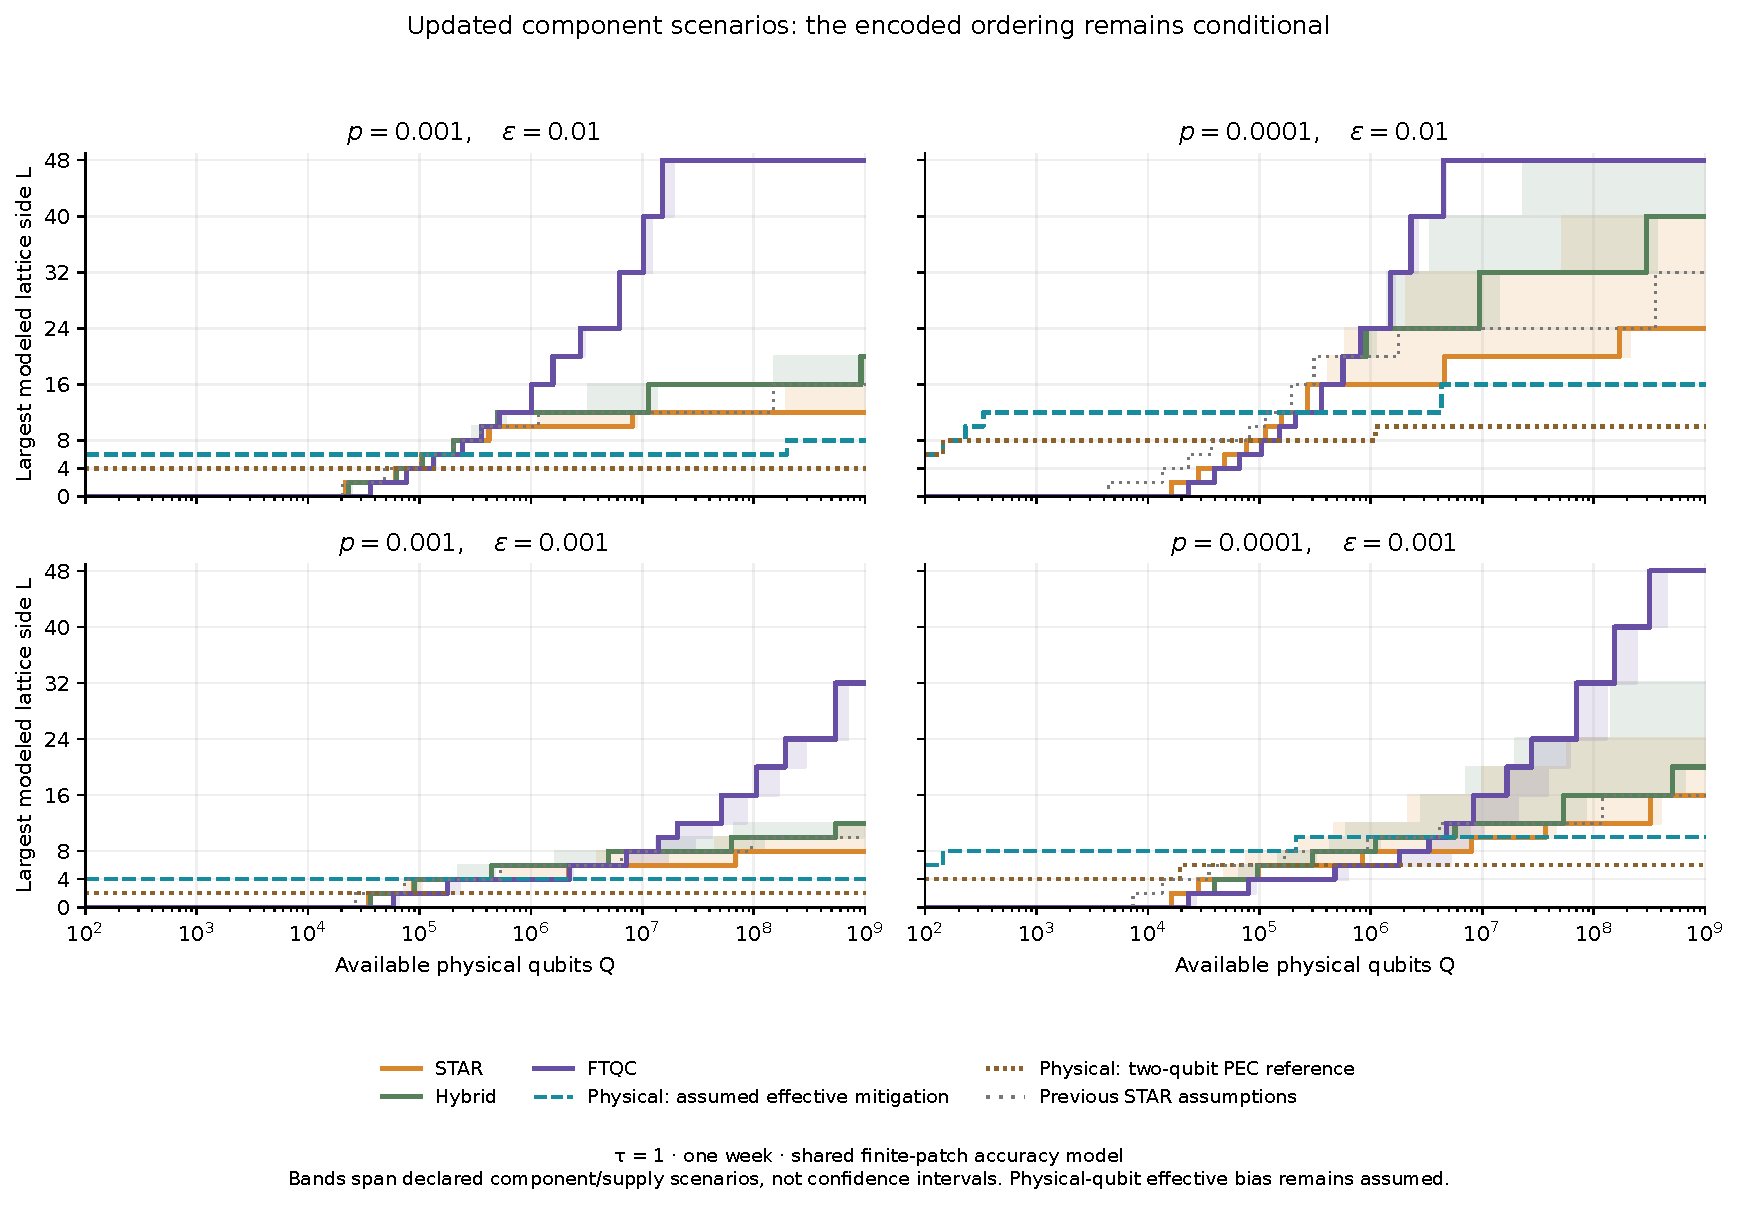
\includegraphics[width=\linewidth]{integrated_capacity.pdf}
\caption{Current component-informed capacity at $\tau=1$ and a one-week cutoff.
STAR and hybrid use angle-dependent generator-fault channels with noisy PCEC,
preparation acceptance, RUS retries, and explicit growth scenarios. FT selects
individual or Hamming-weight synthesis and compact or fast one-port blocks.
Solid encoded curves use growth-campaign upper limits as an independent
component in the analog instrument. Bands include a zero-growth sensitivity
for seed 9 and a slower rejection/supply scenario; they are not confidence
intervals. The previous STAR line is shown for comparison. The NISQ effective
line still assumes that its residual-error reserve is achievable, while the
two-qubit PEC line describes the specified inverse-channel reference.
Larger-lattice Trotter transfer and aggregate delivery remain assumptions;
$L=48$ is the sampled ceiling.}\label{fig:integrated-capacity}
\end{figure}

\paragraph{Injection error and acceptance are coupled.}
Replacing the old coefficient $\alpha=1.5$ with a larger constant would omit
the dependence of preparation cost on angle and injection distance. Instead,
we evaluate the existing restricted instrument at every distinct workload
angle, including noisy probabilistic coherent error cancellation (PCEC) and
repeat-until-success (RUS) corrections. For transverse channel multiplier $c_j$,
the dephasing inverse contributes
\begin{equation}\label{eq:integrated-channel}
 \chi=-2\sum_j\log(\operatorname{Re}c_j),\qquad
 b_{\rm coh}\leq\frac12\left[
 \prod_j\left(1+\frac{|\operatorname{Im}c_j|}{\operatorname{Re}c_j}\right)-1\right].
\end{equation}
Rotation multiplicities enter the sums and products. The coherent term and
finite RUS tail consume explicit error allowance, in addition to the existing
reserve for unmodeled effects. This is a generator-fault submodel with ideal
syndrome projection; detector rejection is still a declared model.

We consider injection seeds 5, 9, and 25, with measured growth anchors at
distances 13 and 25 where available. The central scenario inserts each
seed's simultaneous X/Z campaign upper limit as an independent dephasing
component during growth. Those experiments include memory and readout and
start with an ideally encoded state; their composition with arbitrary-angle
injection is an assumption. Seed 25 avoids growth and pays its own acceptance.
The zero-growth sensitivity is available for seed 9, whose zero observed
failures constrain an upper limit rather than establish zero error. We make
no inference about the untested distance-7 seed.

When the data distance exceeds the growth anchor, we stretch the reference
service time by their distance ratio and charge a further protected handoff.
The extra time and logical volume are explicit, but the corresponding channel
has not been measured. The distance-13 receiver is included to avoid imposing
the distance-25 area at low physical error. Analog parallelism retains the
four-lane aggregate assumption. Cultivation quality and source choices are
shared by FT and hybrid, including the slower-source scenario.

\paragraph{Synthesis is selected before comparing architectures.}
The FT menu includes individual synthesis and Hamming-weight batches 4, 8,
and 16, with workspace and measurement-assisted uncomputation charged.
Compact and fast blocks each have one T-consumption port. The checked
arithmetic savings enter the comparison, while routing remains an aggregate
assumption. The measured slowdown of one explicit onsite transport schedule
is not treated as a full-program correction. Thus changes to the preferred
batch or architecture remain possible when complete schedules are available.

\subsection{Checks against published operating points}\label{sec:published-benchmarks}
Published demonstrations and resource estimates test different parts of the
comparison. We first retain their tasks, estimators and hardware assumptions.
This distinguishes an accounting discrepancy from a change in the scientific
question. In particular, an energy-estimation resource table and a measured
time series do not share the local-observable error contract of
Section~\ref{sec:integrated}.

\subsubsection{The TopQAD STAR and surface-code ledger}
Table IV of Chung et al.~\cite{chung} estimates Hubbard ground-state energies
to error $0.005L^2$. STAR uses quantum complex exponential least squares
(QCELS), while FT uses phase estimation with plaquette Trotterization and
Hamming-weight phasing. Suitable initial ground-state overlap is assumed.
We transcribe all 16 STAR and 32 FT entries. The published distances, retry
clock counts and FT T counts are inputs to this check.

The STAR footprint and the deepest-circuit rotation count are
\begin{equation}\label{eq:published-star-counts}
 Q_{\rm STAR}=(4L^2+1)2d_f^2,\qquad
 R_{\max}=2[8L(L-1)+L^2]r_{\max}.
\end{equation}
For $n=1,\ldots,5$ and $j=1,\ldots,J$, the QCELS time fraction is
$f_{nj}=(n/5)2^{j-J}$ and we use $r_{nj}=\lceil r_{\max}f_{nj}\rceil$.
With 100 samples for each of the real and imaginary quadratures, the
PEC-free evolution-time ledger is
\begin{equation}\label{eq:published-time-ledger}
 T_0=200(d_i+d_f+6)t_{\rm cyc}
 \sum_{j=1}^{J}\sum_{n=1}^{5}
 \bigl[(C_{\rm step}+18)r_{nj}+16\bigr].
\end{equation}
Here $C_{\rm step}$ is the supplied retry-schedule clock count and the
additional terms are the controlled-evolution overhead from Appendix D.
The $350\,\mathrm{ns}$ syndrome round includes six $25\,\mathrm{ns}$ gate
layers plus measurement and reset. The zero-time circuit is omitted from
this evolution-time sum; a physical campaign also prepares and reads out
its samples.

All 16 STAR areas reproduce the published two-significant-digit values.
Fourteen of 16 PEC-free runtimes agree within $2.4\%$. For FT, consuming one
T state per $d_f$ syndrome rounds gives
$T_{\rm FT}=N_Td_ft_{\rm cyc}$, which reproduces all 16 time-optimal entries
within $2.8\%$. This checks consumption given the supplied T count; it does
not reconstruct the private factory and layout optimizer.

\begin{figure}[!htbp]
\centering
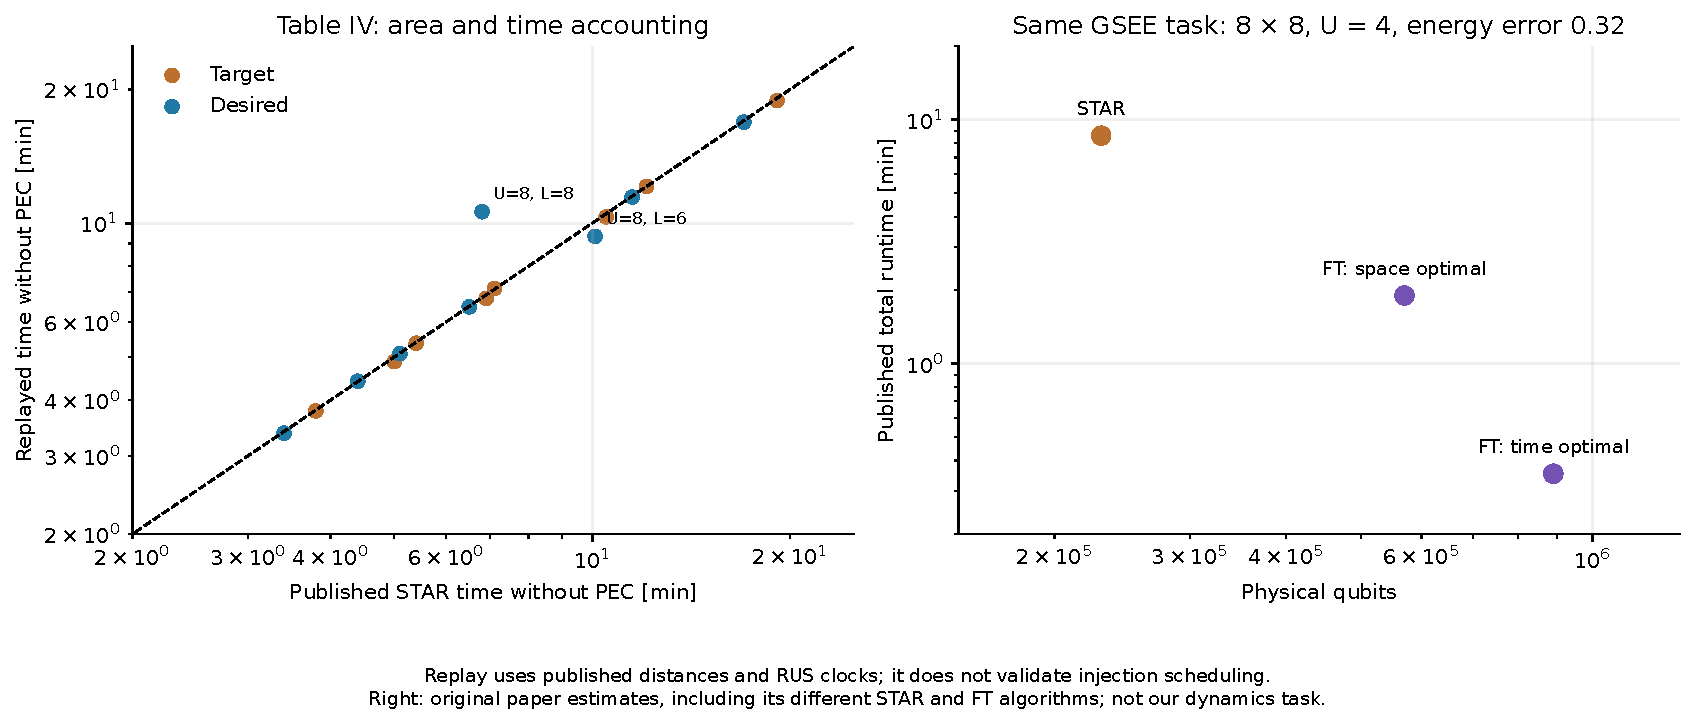
\includegraphics[width=\linewidth]{published_topqad.pdf}
\caption{Published resource accounting on the original energy-estimation task.
Left: STAR campaign times without PEC, reconstructed from the QCELS grid
and supplied gadget clocks. Two desired-hardware entries remain discrepant.
Right: the published $8\times8$, $U=4$ target-hardware estimates show the
area--time tradeoff: STAR uses $230{,}000$ qubits for $8.6$ minutes; FT uses
$570{,}000$ for $1.9$ minutes or $890{,}000$ for $21.2$ seconds. These use
the paper's different STAR and FT algorithms and are not predictions for
our dynamics observable.}\label{fig:published-topqad}
\end{figure}

The growth fit parameters and complete retry schedule have not been
independently reproduced. We instead check their consistency across workloads.
Using the paper's distance-9 small-angle coefficient $\beta$, the PEC
exponent at each QCELS point is
\begin{equation}\label{eq:published-pec}
 \chi(f)=4\beta\Theta_{\max}f+8I_gR(f),\qquad
 \Theta_{\max}=\frac{T_{\max}}{2}
 \left[4L(L-1)+\frac{UL^2}{4}\right],
\end{equation}
where $T_{\max}=0.06/(2\eps/3)$ and $I_g$ is the growth contribution per
state. The factor eight combines the PEC factor four with two growth
contributions per successful rotation. Fitting $I_g$ only at $U=4,L=4$
gives $3.17\times10^{-6}$ for target hardware. Carrying it unchanged to the
other seven target-hardware entries reproduces their total runtimes within
$10\%$. This is a calibrated transfer check, not a forward gadget prediction.

Two desired-hardware entries remain flagged. At $U=8,L=8$, the listed
750 clocks predict $470\,\mathrm{ms}$ rather than the listed
$297\,\mathrm{ms}$. At $U=8,L=6$, the reported total-to-PEC-free ratio
is below the angle-only estimate under these conventions, so no nonnegative
$I_g$ reproduces it. Agreement in total runtime can conceal compensating
differences in its components.

On the fixed target-hardware $4\times4$ workload, changing only the clock
from 350 to $240\,\mathrm{ns}$ multiplies runtime by $0.686$; doubling
$\beta$ multiplies it by $1.13$. Substituting our distance-9-to-13 growth
upper bound instead multiplies it by $5.81$. The last substitution changes
the noise and protocol interpretation and is only a sensitivity. It identifies
growth as the larger unresolved input at this point, rather than providing
a calibrated translation between the two hardware models.

\subsubsection{The Phasecraft/Quantinuum experiment}
We reduce the public shot archive and supplied processed observables for the
$56$-qubit experiment of Alam et al.~\cite{alam2025,phasecraftdata2025}.
Its $7\times4$ periodic lattice has $\pi$ flux and a dimer/defect initial
state, evolved for four Trotter steps. The archive contains 160 shots at
each of 20 times for each of $U=0$ and $U=4$. Direct reconstruction from
the occupation bits reproduces every saved raw mean doublon to floating-point
precision. We retain all 28 local doublons and the spatial mean; no trained
correction or Gaussian-process smoothing is refitted.

For a shot with occupations $n_{i\sigma}$, the spatial estimator is
\begin{equation}\label{eq:experimental-spatial-variance}
 \overline D=\frac{1}{28}\sum_i n_{i\uparrow}n_{i\downarrow},\qquad
 \operatorname{Var}(\overline D)=\frac{1}{28^2}
 \sum_{i,k}\operatorname{Cov}(D_i,D_k).
\end{equation}
At $U=4$, the median raw variance per shot is $0.0035$, compared with
$0.149$ for the mean individual-site Bernoulli variance and our planning
reference $v_*=0.09$. Spatial averaging and correlations thus change the
shot budget substantially. Training and smoothing additionally share
information across circuits and times. The shot arrays do not identify
pseudo-twirling groups, so our pooled variance is a diagnostic; the figure
retains the authors' reported uncertainties, including their treatment of
twirling and processing.

\begin{figure}[!htbp]
\centering
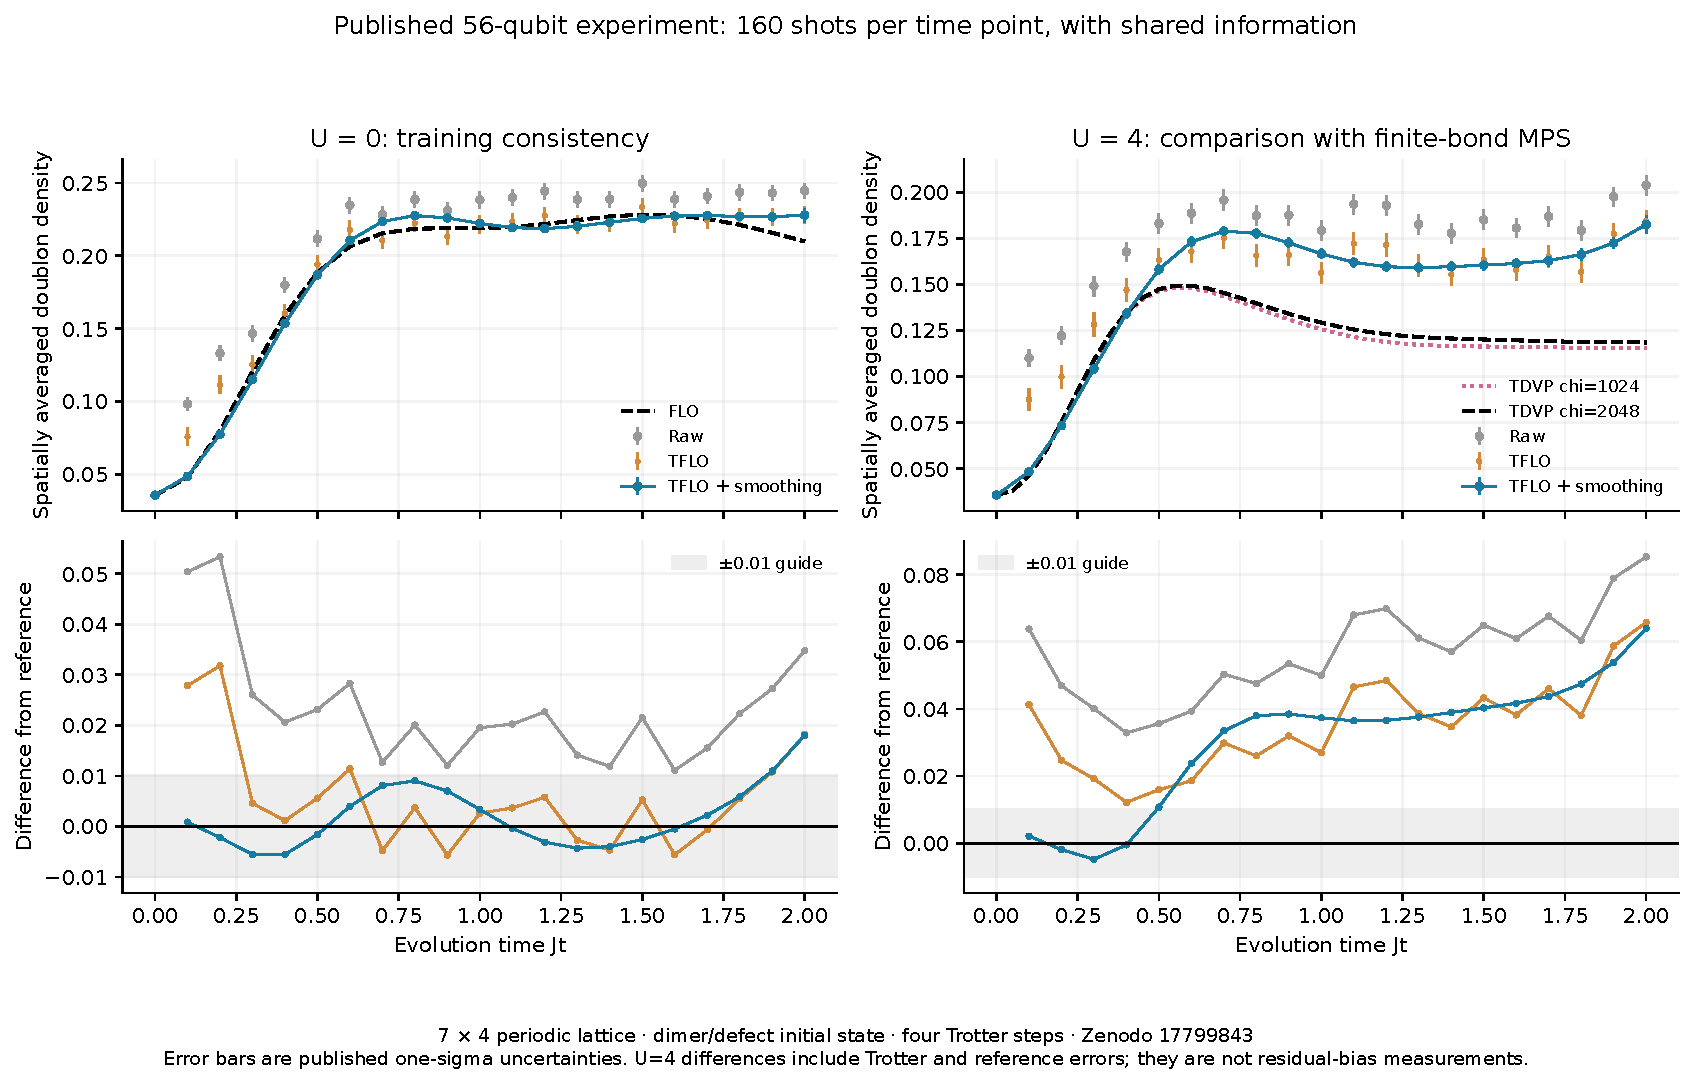
\includegraphics[width=\linewidth]{published_phasecraft.pdf}
\caption{Published experimental estimates and classical references, reduced
from the pinned data archive. All 20 experimental times are shown. The
$U=0$ comparison uses training information and is a consistency check.
At $U=4$, the TDVP curves are finite-bond MPS references, not exact truth;
differences also contain Trotter error and cannot be identified with mitigation
bias. The $\pm0.01$ band is a visual guide, not an accuracy certificate.
Error bars are the published standard errors.}\label{fig:published-phasecraft}
\end{figure}

For the spatial mean at $U=0$, the RMS difference from the FLO reference
drops from $0.0259$ raw to $0.0115$ with TFLO and $0.0064$ after smoothing.
At $U=4$, the corresponding differences from the bond-2048 TDVP reference
are $0.0584$, $0.0378$ and $0.0362$. The latter differences combine
experimental, Trotter and reference errors. For the processed local doublons,
the median reported standard error is $0.0146$, compared with $0.0028$ for
the spatial mean. The useful low-shot experimental curves therefore do not
imply the distinct $0.001$ local-observable contract, while a gatewise PEC
budget for that contract does not predict the experiment's shot count.

These checks establish consistency of published operating points with the
accounting and identify the inputs still requiring prediction: observable
accuracy for a chosen physical estimator, full noisy injection and growth,
and complete magic-state delivery. They do not reduce the architecture scenario
bands to statistical error bars. We next examine the superconducting data,
whose geometry is closer to our baseline.

\subsubsection{Willow: observed accuracy and the sampling design}\label{sec:willow}
The public Willow data~\cite{phasecraftwillow2025,willowdata2025} permit a
direct check across circuit depths and lattice sizes. Our declared selection
contains all center-hole cases at $4\times4$ and $6\times6$, with zero or
$\pi$ flux, $U=0,4,8$, and one to three Trotter steps. Each of the 36 cases
has 24 nonzero evolution times and 200,000 attempted shots per time, organized
as 20 randomized compilations of 10,000 shots. The reduction therefore covers
$172.8$ million attempted shots. These are reused public measurements, not
new quantum runs.

The physical footprint is 34 or 74 qubits, including two ancillas, while
32 or 72 modes encode the fermions. Table I of the paper gives
$G_2=400r+20$ at $4\times4$ and $G_2=1440r+52$ at $6\times6$.
At three steps these are 1220 and 4372 two-qubit gates. The circuit scale
is consistent with our native-gate proxy. Its estimator, however, uses
selection, training, symmetry and shared time-series information. A single
time series costs $4.8$ million attempted shots, with an additional $U=0$
training series whose cost can be shared by interacting targets.

\begin{figure}[!htbp]
\centering
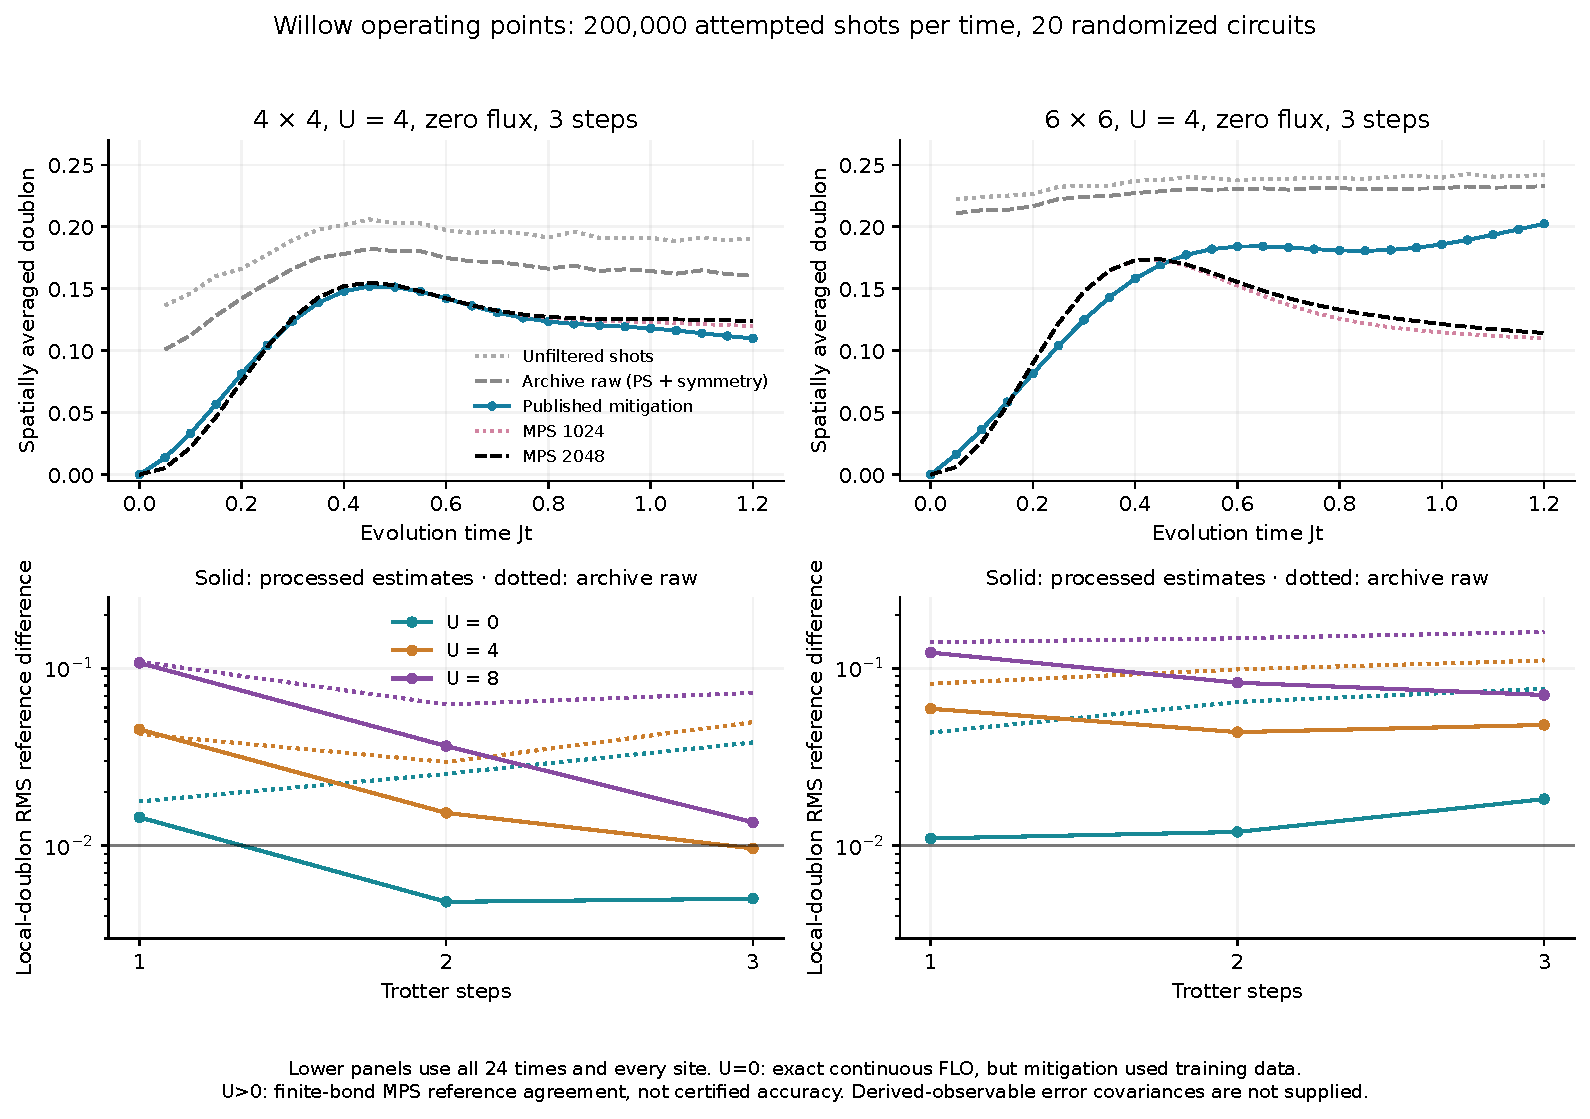
\includegraphics[width=\linewidth]{willow_operating_points.pdf}
\caption{Willow experimental operating points. Upper panels show the spatial
mean doublon at $U=4$, zero flux and three steps, with finite-bond MPS
references. Lower panels compare all local doublons at all 24 measured times
as the step count changes. The $U=0$ reference is independent continuous
free-fermion evolution, but the experimental estimator uses $U=0$ training.
The interacting references are approximate MPS calculations. Differences
are not certified experimental errors, and the $0.01$ line is a guide.}
\label{fig:willow-operating}
\end{figure}

For $U=4$, zero flux and three steps, processed local doublons differ from
the bond-2048 reference by $0.0096$ RMS at $4\times4$ and $0.0479$ at
$6\times6$. For the spatial means the differences are $0.0068$ and $0.0451$.
The median reported standard errors of the constituent local $Z$ estimates
are $0.0156$ and $0.0810$, respectively. These observed operating points
help explain a useful physical-qubit calculation with tens of qubits, while
leaving the stricter accuracy requirement in our architecture comparison open.
The interacting exact-reference groups are empty in this archive, despite
the paper showing exact $4\times4$ comparisons. We therefore retain the
approximate-reference qualification even at $4\times4$.

Two archive conventions affect the comparison. First, values labeled
\texttt{raw} already include number selection and diagonal symmetry averaging.
The randomized-compilation means must receive equal weight after rejection;
pooling all accepted shots gives different weights. We reproduce these raw
means in all 36 workloads, with number-deviation thresholds of zero at
$4\times4$, two at zero-flux $6\times6$, and one at $\pi$-flux $6\times6$.
Second, the $U=0$
\texttt{exact} values change with step count and describe the free circuit,
not continuous dynamics. We compute a separate continuous FLO reference by
orbital evolution, checked against the existing many-body sector solver.
The supplied initial-state JSON is inconsistent with the center-hole labels;
we instead identify and check the product input from its zero-time reference
occupations. These distinctions are recorded in the data audit.

The processed archive supplies marginal $Z$ and $ZZ$ errors, without their
cross-covariances. For a derived observable $O=\sum_i c_i O_i$, we retain
the covariance-independent upper bound
\begin{equation}\label{eq:willow-derived-se}
 \operatorname{SE}(O)\leq\sum_i |c_i|\operatorname{SE}(O_i).
\end{equation}
We do not infer independent sites or treat this statistical bound as a bound
on total error. The figures show the derived central values rather than
presenting that loose bound as a measured confidence interval.

\paragraph{Additional sampling must specify what is repeated.}
Shots of one randomized circuit share its noise realization. Let $K$ be the
number of independent randomized circuits, $a$ the variance of their
conditional expectations, and $v/n$ the typical variance of each conditional
sample mean. A useful planning decomposition is
\begin{equation}\label{eq:willow-sampling}
 \operatorname{Var}(\widehat O)\simeq\frac{a+v/n}{K}.
\end{equation}
Increasing $n$ at fixed $K$ leaves the $a/K$ contribution. Increasing the
number of independent circuit realizations reduces both contributions.
We estimate them from the 20 recorded groups, retaining acceptance, and
separate that planning extrapolation from the directly measured variance of
their mean. The inferred $a$ is uncertain and is not an irreducible hardware
error floor.

\begin{figure}[!htbp]
\centering
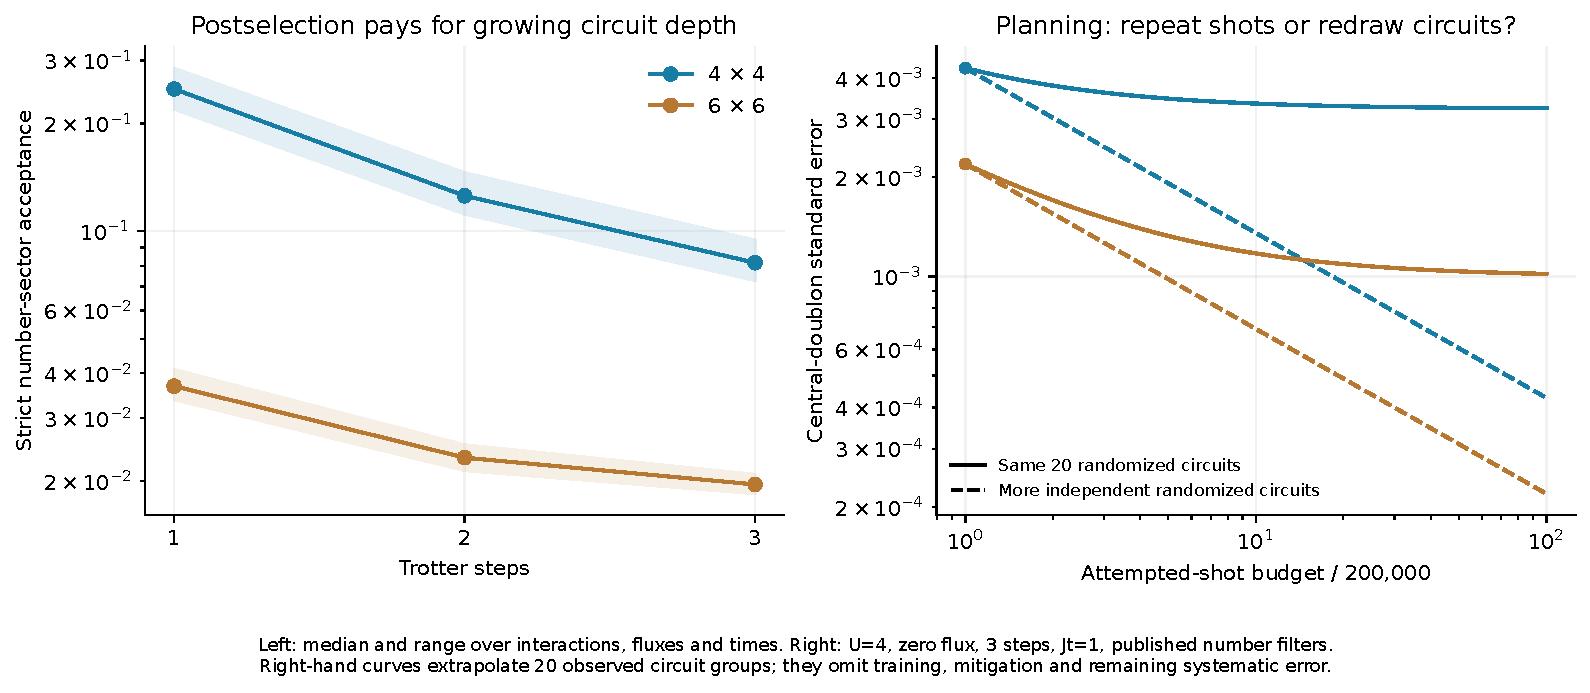
\includegraphics[width=\linewidth]{willow_sampling_design.pdf}
\caption{Measured acceptance and a sampling-design sensitivity. Left: strict
number-sector acceptance, with median and range across the declared times,
fluxes and interactions. Right: the central doublon's sampling uncertainty
at $U=4$, zero flux, three steps and $Jt=1$, before TFLO and smoothing.
The right panel retains the corresponding published number filter: exact
sector at $4\times4$ and up to two total number deviations at $6\times6$.
Dots show standard errors across the observed circuit groups. Curves
extrapolate Equation~\eqref{eq:willow-sampling}, assuming independent new
groups with the same distribution. They do not predict mitigation accuracy.}
\label{fig:willow-sampling}
\end{figure}

The experimental comparison therefore constrains the physical arm at two
levels: a directly measured circuit and sampling cost, and an
observable-dependent comparison with available references. It supports useful
small-footprint dynamics without certifying every local observable at
$0.01$ or $0.001$. We now calculate a matched interacting reference for
the main $4\times4$ example.

\subsubsection{Separating circuit error from experimental discrepancy}\label{sec:willow-reference}
For the $4\times4$, $U=4$, zero-flux center-hole input, we compute both
continuous Hamiltonian dynamics and the ideal experimental circuits at all
24 saved times and all three step counts. This input has seven up spins,
eight down spins and a hole at $(1,1)$; it differs from the half-filled
N\'eel input in our resource baseline. Its fixed-particle sector contains
$\binom{16}{7}\binom{16}{8}=147232800$ amplitudes.

The circuit uses the hopping order specified by the swap network in
Appendix D2 of Ref.~\cite{phasecraftwillow2025}. In a fixed fermionic frame,
each step is an ordered half sweep of hopping terms, all onsite rotations,
and the reverse hopping half sweep. Independent orbital evolution reproduces
the archived $U=0$ circuit references at all 288 saved combinations of size,
flux, step count and time. This check requires the archive's diagonal symmetry
averaging: the maximum local-$Z$ discrepancy falls from $0.345$ without
averaging to below $6\times10^{-15}$ with it. We apply the same averaging
to the interacting circuit observables.
For this input and zero-flux Hamiltonian, diagonal reflection leaves the
continuous target unchanged. The ordered finite-step circuit can break that
symmetry, so applying the averaging to its reference matters.

Continuous evolution uses matrix-free Chebyshev propagation in increments
of $0.05$, with a conservative spectral bound of $64$. We retain the
analytical state-truncation bound and check floating-point behavior through
full-state comparisons with independent small-system Fock-space calculations
and a separate direct propagation to $Jt=1$. Ideal circuits use exact
two-mode hopping and onsite phase updates. These are numerical references
for the specified finite-system unitary, not noisy hardware simulations.

Let $D_H$ denote continuous dynamics, $D_C$ the ideal circuit result, and
$\widehat D$ the published experimental estimate. Then
\begin{equation}\label{eq:willow-error-decomposition}
 \widehat D-D_H=(\widehat D-D_C)+(D_C-D_H).
\end{equation}
The first contribution contains finite sampling and experimental processing
effects. The second is deterministic circuit error. Squaring and averaging
therefore retains a cross term; the two RMS differences cannot be added or
interpreted as independent error bars. We report observed discrepancies
without identifying them with the ensemble bias of an estimator.

The two contributions respond oppositely to refinement:
\begin{center}
\small
\begin{tabular}{rrrr}
\toprule
Steps & Experiment--circuit RMS & Circuit--continuous RMS & Total RMS\\
\midrule
1 & $0.00469$ & $0.04481$ & $0.04429$\\
2 & $0.00764$ & $0.01973$ & $0.01581$\\
3 & $0.00946$ & $0.01315$ & $0.01030$\\
\bottomrule
\end{tabular}
\end{center}
More steps improve the ideal dynamics while the observed circuit discrepancy
grows. At three steps the total RMS is smaller than the circuit error alone
because the signed contributions partially cancel. This is a measured
depth--accuracy tradeoff in the tested experimental pipeline, not a
projection of its performance beyond three steps.

At three steps, $71.4\%$ of the 384 local time-site points lie within
$0.01$, while the largest difference is $0.0400$. The bond-2048 MPS reference
differs from continuous dynamics by $0.00214$ RMS and at most $0.00909$.
Thus its previous use gave a reasonable overall accuracy scale, but could
not resolve a $0.001$ comparison. These statements concern the saved data
set; they are not statistical coverage guarantees.

\begin{figure}[!htbp]
\centering
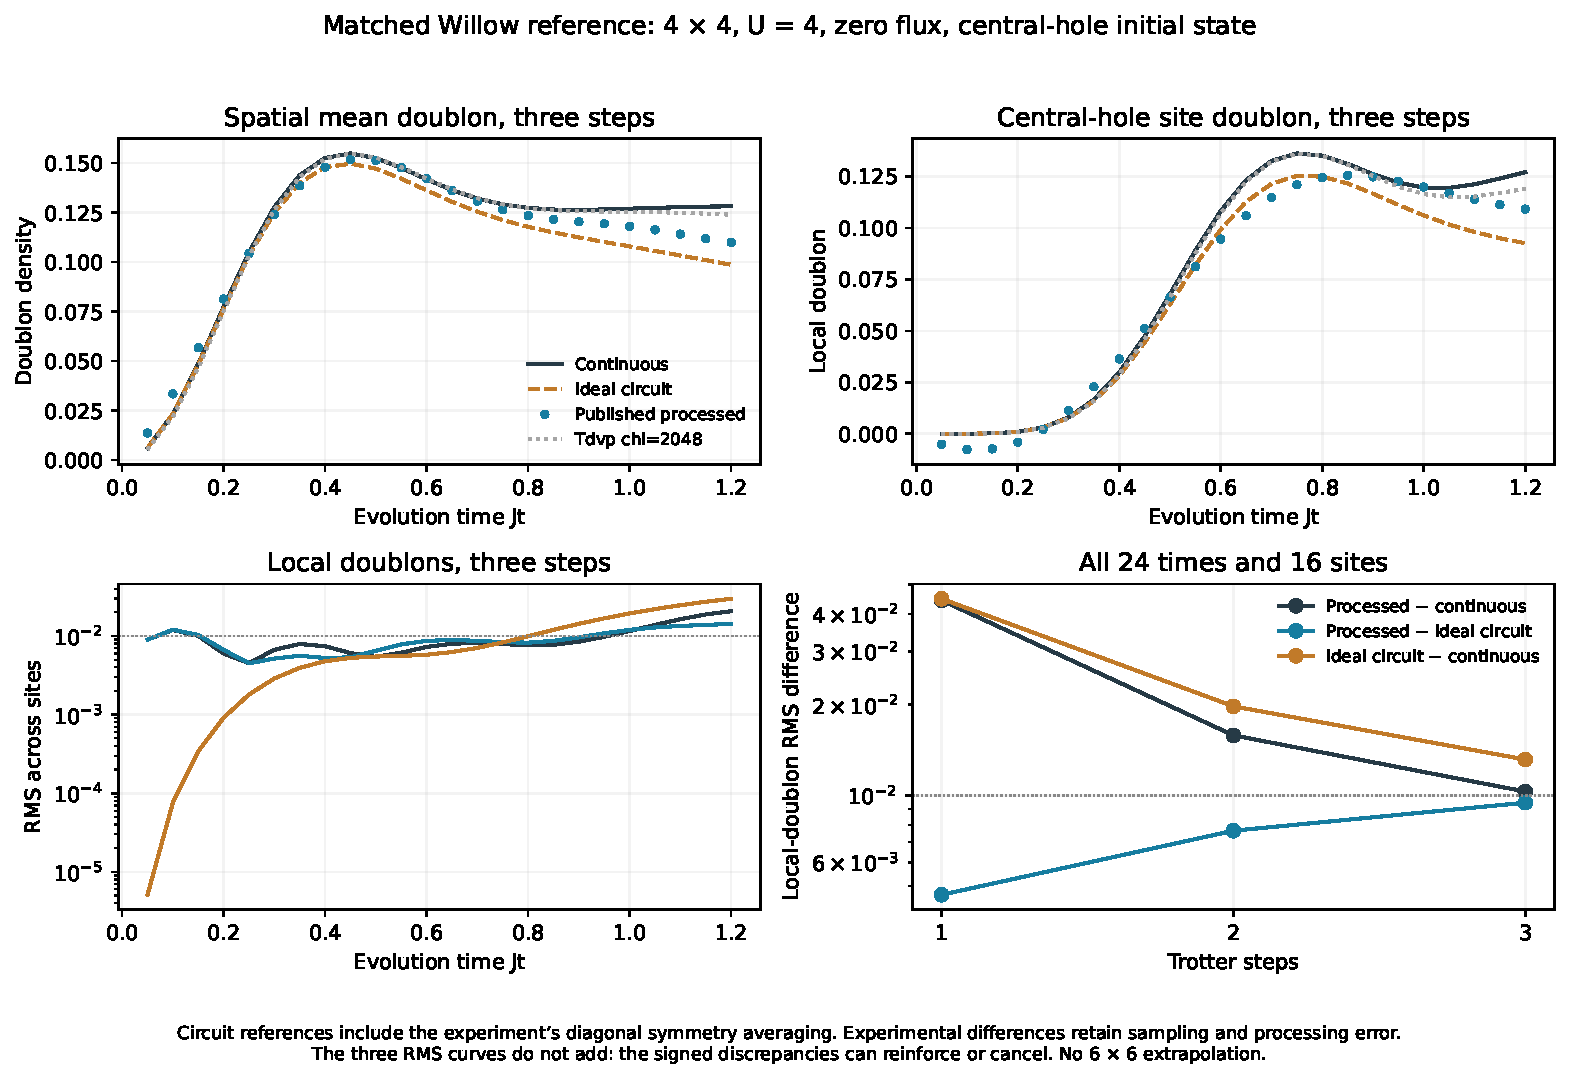
\includegraphics[width=\linewidth]{willow_matched_reference.pdf}
\caption{Matched interacting reference for the $4\times4$, $U=4$, zero-flux
center-hole experiment. Upper panels: spatial mean and central-site doublons
at three steps. Lower left: local-doublon RMS differences across sites at each
time. Lower right: RMS differences
over all 24 times and 16 sites versus step count. The ideal circuit includes
the same diagonal averaging as the processed estimates. Signed discrepancies
can reinforce or cancel, so the three RMS curves do not add. The experimental
curves retain finite sampling and processing error; no larger-lattice transfer
is assumed.}\label{fig:willow-reference}
\end{figure}

This comparison tests useful dynamics on the experiment's actual small
device. It neither substitutes a fitted mitigation exponent into the capacity
model nor transfers this input's Trotter coefficient to the N\'eel baseline.
The distinction between a roughly $0.01$ RMS experimental result and a
specified local-observable error budget remains central to comparing the
physical and encoded architectures.

\clearpage
\subsection{Earlier physical-error and algorithm sensitivities}\label{sec:physics-sweep}
This section retains the previous scalar-coefficient comparison. Its numbers
are historical controlled sensitivities; Section~\ref{sec:integrated} is the
current integrated result.
We lead the workshop example with $0.01$ absolute error on the local doublon
observable and retain $0.001$ as a second principal target. Figure~\ref{fig:p-capacity}
varies $p$ from $10^{-3}$ to $10^{-4}$ while keeping the clocks, Hamiltonian,
initial state, observable, and finite-patch Trotter model fixed. The $p=10^{-3}$
central rows reproduce all 144 corresponding entries of the previous
added-patch comparison. The new sweep contains 864 scenario points, with
per-arm error allocation and source counts reoptimized. The model remains a
finite-lattice workload comparison: at fixed time, an independently justified
local-patch approximation could change what increasing $L$ means.

\begin{figure}[t]
\centering
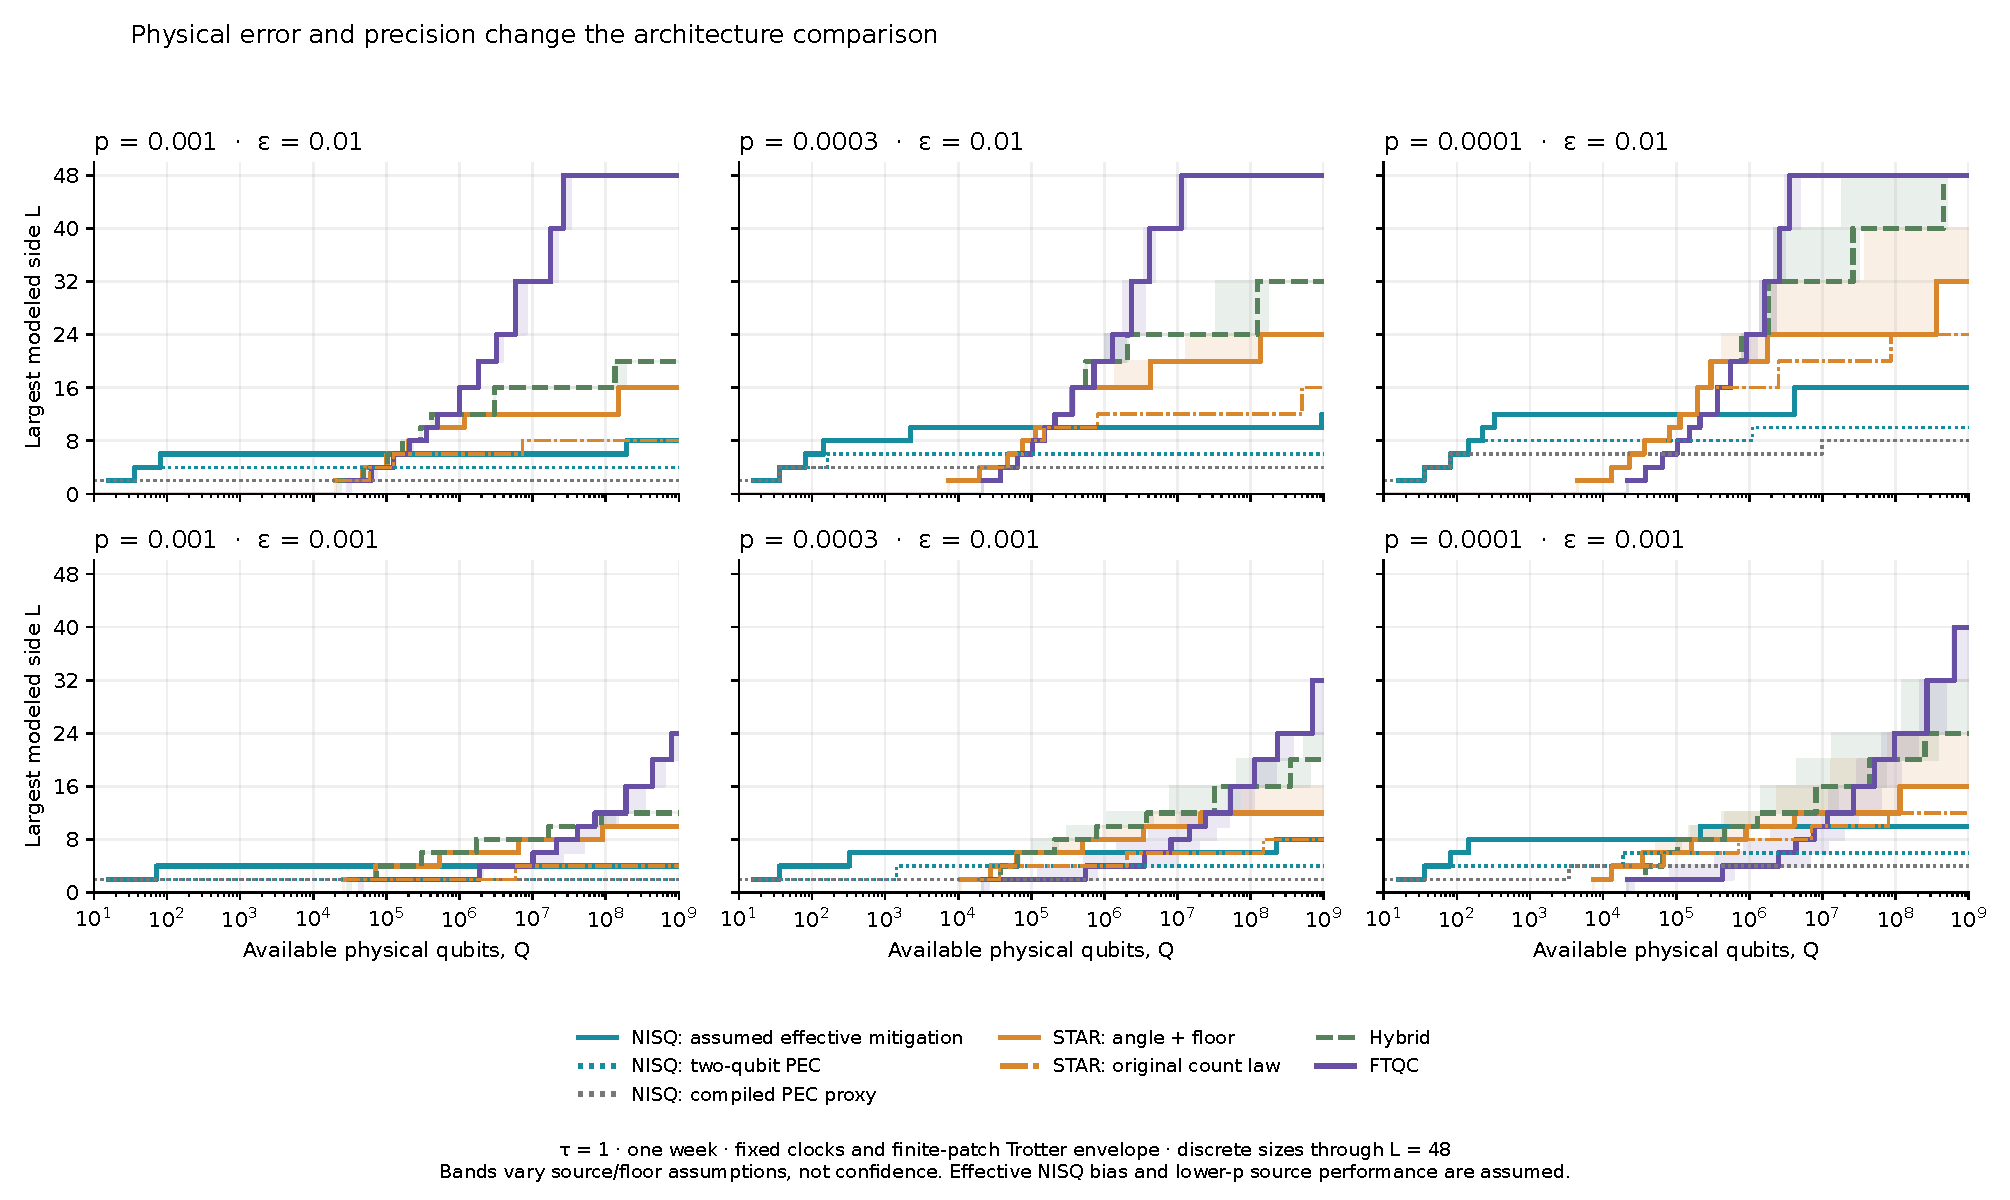
\includegraphics[width=\linewidth]{physical_error_capacity.pdf}
\caption{Achievable lattice side versus available physical qubits at $\tau=1$
and a one-week cutoff. Columns vary physical error; rows show $0.01$ and
$0.001$ absolute error. Solid encoded curves retain the source and injection
floor at their $p=10^{-3}$ reference values. Bands span the explicit
source/floor scenarios described in the text, not statistical confidence
intervals. The count-law STAR curve changes the injection exposure while
retaining the same delivery model. NISQ retains separate assumed-effective,
two-qubit PEC, and compiled-PEC scenarios. Only the sampled sizes are shown;
$L=48$ is the sweep ceiling. Larger-lattice accuracy transfer and effective
mitigation bias remain assumptions.}\label{fig:p-capacity}
\end{figure}

\paragraph{Source assumptions remain visible.}
We do not infer a new cultivation protocol from a change in $p$. The held
scenario keeps $q_T=2\times10^{-9}$, a 1024-qubit source, 100 preparation
cycles, and the distance-15 handoff constraint. A second scenario assumes
$q_T(p)=2\times10^{-9}(p/10^{-3})^3$ and an injection floor
$f(p)=10^{-5}(p/10^{-3})$, with source area and cycles unchanged. A third
keeps both error floors fixed and multiplies source preparation cycles by
four. These choices bracket specified sensitivities; they are not calibrated
lower-$p$ implementations or guaranteed bounds on an optimal source.
In particular, the inherited handoff convention imposes $d\geq15$ on the
FT/hybrid data block as well, so its low-$p$ area floor is a model choice.
The ideal cleanup term $35q_T^3$ accounts for input-state errors. Faults in
the cleanup block and waiting storage are charged separately through the
protected tile-time volume and logical-error budget.

At $Q=10^6$ and $\eps=0.01$, lowering $p$ from $10^{-3}$ to $10^{-4}$
raises the held-scenario STAR capacity from $10\times10$ to $20\times20$,
and FT/hybrid capacity from $12\times12$ to $24\times24$. The NISQ
effective and two-qubit PEC capacities increase from sides 6 and 4 to
12 and 8, respectively. At $\eps=0.001$, the corresponding STAR and FT
sides are 6 and 2 at $p=10^{-3}$, and 10 and 4 at $p=10^{-4}$.
The latter comparison is sensitive to the magic-state assumption: for the
strict $4\times4$ FT task at $p=10^{-4}$, holding $q_T$ fixed costs
$4.23\times10^5$ qubits, whereas the assumed cubic improvement gives
$8.47\times10^4$. Lower physical error benefits every arm, but the relative
window cannot be specified by $p$ without the source assumptions.

\paragraph{Injection law as a controlled switch.}
For the original injection model~\cite{akahoshi}, we use the exact
dephasing-inverse exposure
\begin{equation}\label{eq:count-law-switch}
 \chi_{\rm count}=-2R\log(1-8p/15),
 \qquad
 \chi_{\rm angle}=4\alpha p\Theta+4fR.
\end{equation}
Both calculations use the same surface-code law and delivery timing, so
this switch isolates the exposure law rather than reconstructing two
complete physical protocols. At $p=10^{-3}$, the optimized strict
$4\times4$ STAR estimate changes from $7.14\times10^4$ qubits under
the angle law to $5.87\times10^6$ under the count law. At $p=10^{-4}$,
both estimates fit in one $13{,}122$-qubit copy. Thus a change in the
injection law can dominate the strict comparison at the original noise
point without producing a fixed architecture advantage at all $p$.

\paragraph{Repeated-angle synthesis changes the FT comparison.}
We implement Campbell's Hamming-weight phasing construction for equal-angle
rotations within each plaquette stage~\cite{campbell}. A batch of $b$
rotations uses
\begin{equation}\label{eq:hwp-resources}
 a_b=b-\operatorname{popcount}(b),\qquad
 k_b=\lfloor\log_2 b\rfloor+1
\end{equation}
clean ancillas/measurement-assisted Toffolis and synthesized rotations,
respectively. We charge four $T$ states per Toffoli, synthesize all $k_b$
weight-register rotations within the common error budget, and reuse the
$a_b$ ancillas between batches. The peak workspace is charged for the full
shot; arithmetic adds two logical Clifford clocks per Toffoli to the
reference timing model. We retain all fixed plaquette $T$ gates and do not
pool equal angles from different times. Batch size one exactly reproduces
individual synthesis. The nearest-neighbor surgery layout and effective
delivery ports remain uncompiled reference assumptions.

\begin{figure}[t]
\centering
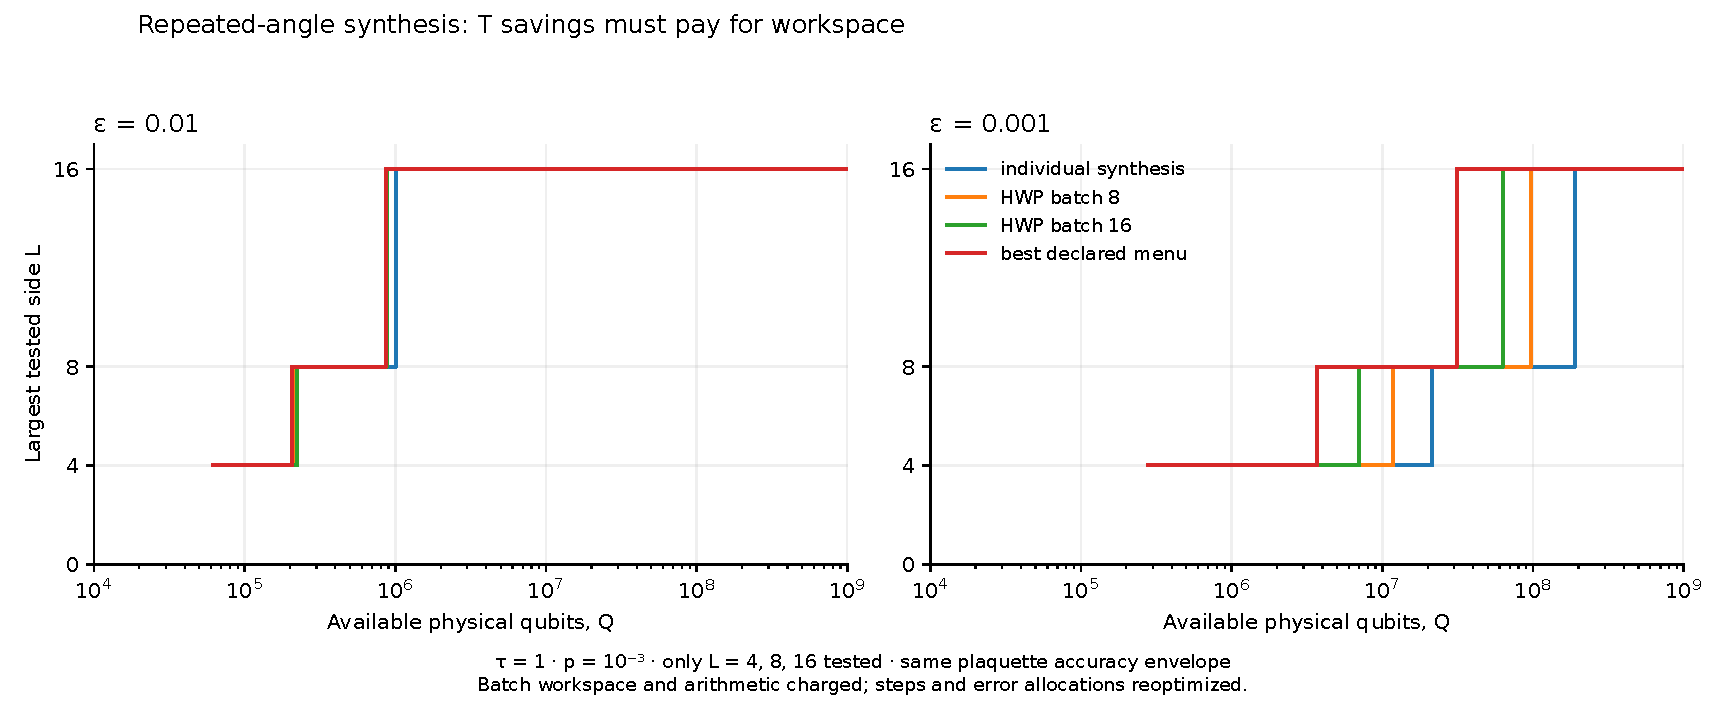
\includegraphics[width=\linewidth]{hamming_weight_comparison.pdf}
\caption{FT capacity with repeated-angle synthesis, for the three tested
lattice sides 4, 8, and 16. The best-menu curve chooses individual synthesis
or an allowed Hamming-weight batch, with steps and error budgets reoptimized.
The circuit, plaquette accuracy envelope, source menu, and delivery convention
are common. The staircase ends at the largest tested size; it is not an
FT capacity plateau.}\label{fig:hwp-capacity}
\end{figure}

At $p=10^{-3}$ and $\eps=0.001$, batch size 16 reduces the
$4\times4$ estimate from $1.88\times10^6$ to $2.78\times10^5$ qubits.
The optimized circuits consume 192,332 and 80,123 $T$ states per shot,
with 33 and 36 steps, respectively; the latter uses 15 extra logical
ancillas. The area improvements at $L=8$ and 16 are factors 5.78 and
6.04, using batches of 64 and 63 live ancillas. At $\eps=0.01$,
individual synthesis remains cheaper at $L=4$ and 8 because one copy
already completes the campaign and the extra workspace raises its area.
These results change the strict FT comparison substantially without
changing the Hamiltonian simulation algorithm. The principal $p$ sweep
deliberately retains individual synthesis to preserve its frozen baseline.

At strict $4\times4$, neither selected circuit uses a cleanup stage.
The lower $T$ demand reduces the magic-state error allocation from 38.5\%
to 16.0\% and increases the statistical allocation from 29.8\% to 58.0\%.
The reduced shot count explains why the area gain exceeds the reduction in
$T$ count: repeated-angle synthesis changes the optimal estimator budget as
well as the cost of a circuit.

\paragraph{Local encoding and local ordering are different changes.}
The compact encoding maps hopping to Pauli operators of weight at most
three and uses fewer than 1.5 qubits per fermionic mode on the square
lattice~\cite{derbyklassen}. We evaluate a $3N$-qubit register scenario,
with four CNOTs per hopping Pauli and two per onsite Pauli, plus $8N$
assumed preparation gates. A two-CNOT hopping variant assumes fusion;
a routing variant doubles movement and placement costs. Preparation,
embedding of both spin sectors, and gate utilization are explicitly
uncompiled assumptions. The generic parity gadgets use 6,754 two-qubit
gates at $L=4,r=8$, compared with approximately 3,455 in the native
JW proxy. The fused hypothesis uses 3,682. Removing asymptotic routing
growth therefore does not guarantee savings at the small lattices
accessible under the present noise assumptions.

For STAR, the compact scenario enlarges the data register and separately
tests four and sixteen assumed rotation lanes. Four lanes cost more area
than the JW reference at $L=4$, and sixteen lanes cost still more because
the selected calculation already fits in one copy. Locality does not
automatically pay for parallel delivery. These resource scenarios retain
the existing termwise error envelope; transferring it to larger lattices
remains an assumption.

A separate exact-sector diagnostic isolates ordering. Keeping the
Hamiltonian, initial state, JW representation, and original onsite split
fixed, a four-color bond permutation changes the $\tau=1$ coefficient
$|D_r-D|r^2$ from approximately 0.0344 to 0.0463 on $2\times2$ and
from 0.0766 to 0.0913 on $3\times3$. Grouping all onsite terms instead
gives 0.2231 and 0.2178, matching the plaquette results on these patches.
These measurements show that a more parallel ordering need not reduce
the local-observable error. They neither establish bulk convergence nor
replace the frozen accuracy envelope.

\subsubsection{Qubitized dynamics for the same Hamiltonian}\label{sec:qsvt-comparison}
We also count a qubitized implementation of the open-boundary Hamiltonian,
using pyLIQTR and Qualtran components with quantum singular value
transformation (QSVT)~\cite{gilyen2019,babbush2018}. The specialized Hubbard
encoding in the installed library has periodic boundaries; using it directly
would change the task. The centered open-boundary Pauli expansion instead has
\begin{equation}
 \alpha=\sum_\ell |h_\ell|=4L(L-1)+\frac{U}{4}L^2,
 \qquad \alpha\big|_{L=4,U=4}=64.
\end{equation}
At $U=4$, hopping coefficients have magnitude $1/2$ and onsite coefficients
have magnitude one. Repeating each onsite Pauli twice makes all LCU weights
equal. There are $8L(L-1)+2L^2$ entries, exactly 128 at $L=4$, so PREPARE
requires only seven Hadamards there. The controlled block encoding costs
508 T gates and no arbitrary rotations. Generic amplitude preparation at
the same point costs 508 T gates plus 256 arbitrary rotations. A local
adapter places coefficient signs in SELECT and magnitudes in PREPARE;
zero-weight padding selects the identity. The Hamiltonian is independently
checked against full fermionic creation and annihilation operators on
$2\times2$.

We use half-amplitude cosine and sine polynomials and combine their
controlled branches, giving accepted amplitude $1/4$ before amplification.
The accounting includes rejected attempts, zero through three oblivious
amplification steps, polynomial and phase-realization error, rotation
synthesis, conditional logical-fault bias, and the shared magic-state source
menu. Appendix~\ref{app:qsvt-budget} gives the approximation budget.
These are constructive polynomial and compiled-component counts; large-degree
phase lists and routed SELECT circuits have not been validated. Both algorithms
use the fast data block here. A QSVT sensitivity either omits extra Clifford
serialization or charges all counted Cliffords plus two Clifford slots per T;
neither choice is a physical nearest-neighbor SELECT schedule.

\begin{figure}[t]
\centering
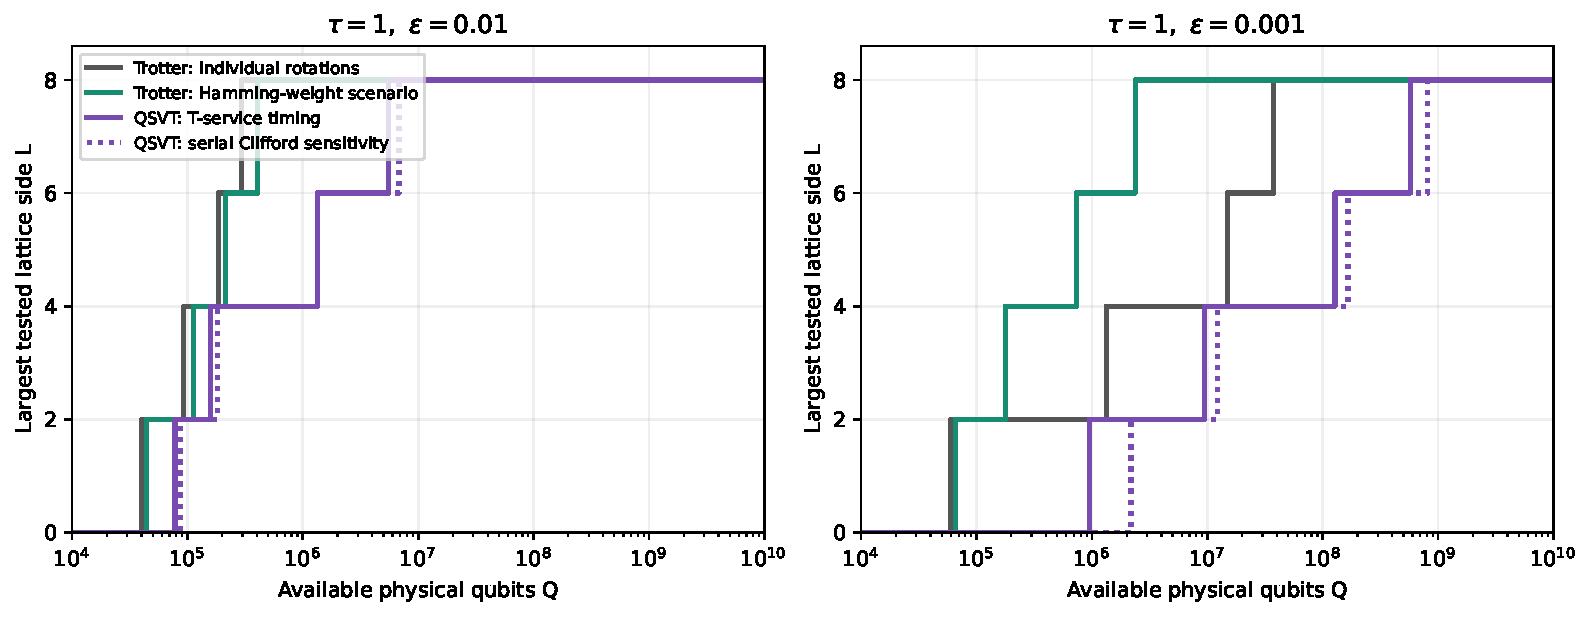
\includegraphics[width=\linewidth]{frontier_algorithms.pdf}
\caption{Same-task FT algorithm comparison at $p=10^{-3}$ and one week.
The vertical coordinate is the largest tested side among $L=2,4,6,8$;
the plateau at eight is the test ceiling. Trotter uses the finite-patch
accuracy envelope and optimized budgets, with individual synthesis or the
aggregate Hamming-weight scenario. QSVT uses the cheaper of the repaired
generic and equal-weight encodings, with state selection and amplification
charged. The dotted curve adds Clifford serialization. These conditional
costs do not include a fully routed SELECT or full Hamming-weight layout.}
\label{fig:frontier-algorithms}
\end{figure}

At $L=4,\tau=1,\eps=0.001$, the selected QSVT circuit uses 551,403 T
states per attempt and costs $9.51\times10^6$ physical qubits under the
T-service timing assumption. Individual Trotter uses 192,332 T states and
$1.34\times10^6$ qubits; the Hamming-weight scenario uses 82,336 T states
and $1.77\times10^5$ qubits. At $\eps=0.01$, the respective QSVT and
individual-Trotter costs are $1.60\times10^5$ and $9.29\times10^4$ qubits.
QSVT does not beat the better Trotter scenario at any of the 32 tested
size, time, and precision points. This comparison does not exclude a more
structured open-boundary encoding or a coherent observable estimator.
The $\tau=8$ Trotter comparison still uses only the $3\times3$ time envelope,
so its transfer to larger lattices remains particularly uncertain.

\subsection{Testing the assumptions behind the capacity curves}\label{sec:implementation}
The capacity comparison depends on three implementation claims: that a
physical estimator can afford its residual bias, that an angle-dependent
STAR source retains favorable error and acceptance after correction and
growth, and that FT arithmetic savings survive delivery and routing.
A fourth question is whether a smaller physical patch can reproduce the
chosen observable. We test each claim with a bounded calculation. These
checks add evidence at their stated scale; they do not silently replace
the full-campaign assumptions in Fig.~\ref{fig:p-capacity}.

\subsubsection{NISQ: an estimator with measured residual bias}
We simulate the full eight-qubit density matrix of a $2\times2$ plaquette
circuit, including the native nearest-neighbor route, gate depolarization,
idle noise, preparation, and readout. The noise convention is $p_2=p$,
$p_1=p/10$, and idle error $p$ per 100\,ns. Spin-number selection retains
outcomes with the correct up/down occupations. Following the training
principle used in the experimental literature~\cite{phasecraftwillow2025},
we fit an affine correction to six noninteracting ($U=0$) circuits and
hold out all interacting tests ($U=2,4$). Training times differ from test
times. Zero-angle interaction slots remain noisy, so the training circuits
do not receive a cheaper noise history.

For selected mean $D$ and acceptance $A$, the asymptotic variance per
physical attempt is $D(1-D)/A$. If the affine estimator is $a+bD$, its test
variance is multiplied by $b^2$. Each of the six training circuits receives
$10^6$ attempted shots in the resource model. With training uncertainty
$V_{\mathrm{train}}$ propagated through both fitted coefficients, we choose
\begin{equation}
 S=\left\lceil\frac{b^2D(1-D)/A}
 { (\eps_{\mathrm{stat}}/1.96)^2-V_{\mathrm{train}}}\right\rceil,
 \qquad \eps_{\mathrm{stat}}=0.0025,\label{eq:trained-shots}
\end{equation}
when the denominator is positive. The fit uses population noisy training
means to isolate systematic transfer error; an independent binomial
training simulation checks the finite-shot variance approximation. The
resource time charges the full training campaign to each test circuit.

\begin{figure}[t]
\centering
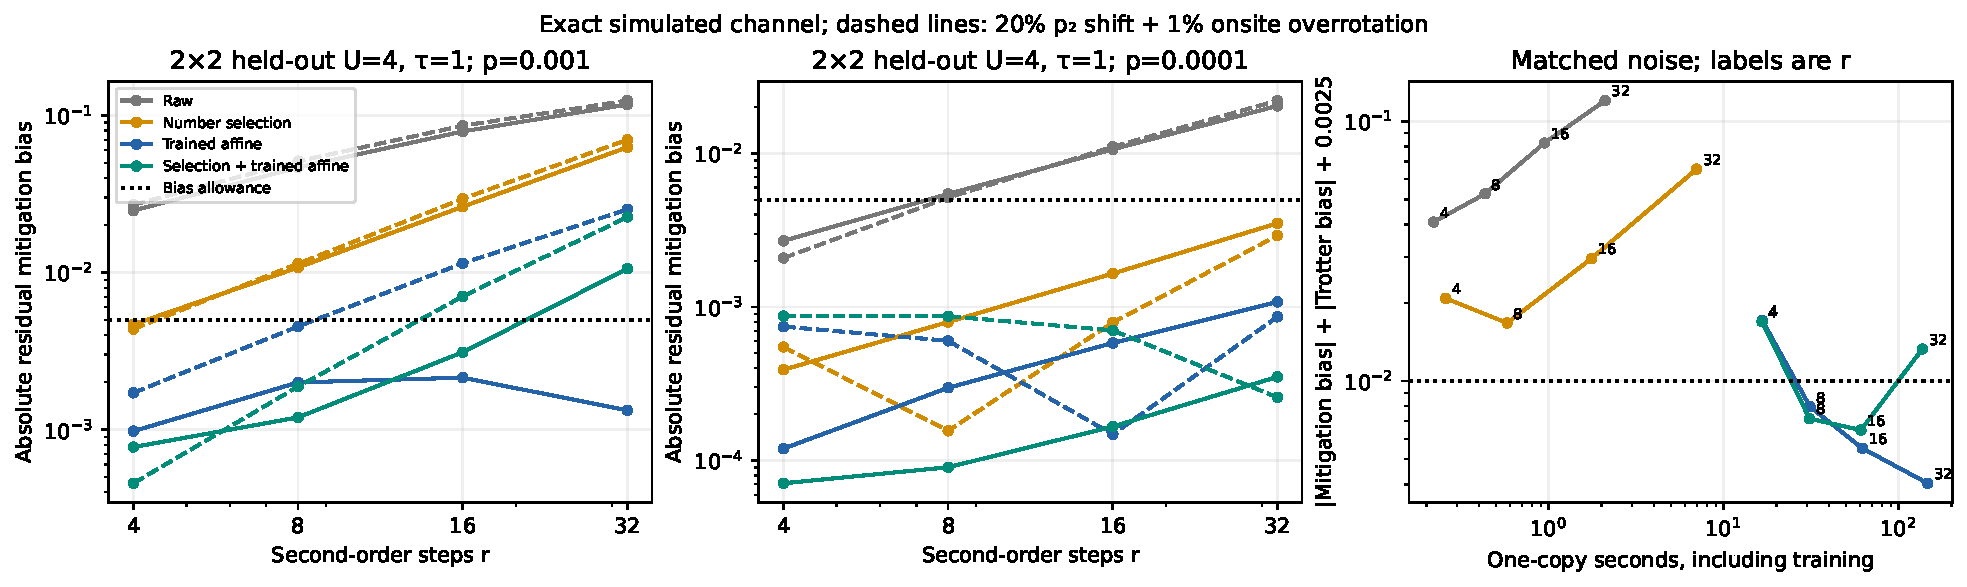
\includegraphics[width=\linewidth]{implementation_nisq.pdf}
\caption{Held-out $2\times2$ estimator checks. The left panels show residual
bias from the ideal circuit, separately from Trotter error. Dashed curves
increase test-circuit two-qubit noise by 20\% and onsite angles by 1\%,
without retraining. The right panel adds absolute mitigation and Trotter
biases to the Gaussian statistical allowance and charges training time.
Labels give the step count. The channel is simulated exactly; the shot
plan is a Gaussian/delta-method approximation. No large-lattice or hardware
accuracy guarantee follows.}\label{fig:implementation-nisq}
\end{figure}

At $p=10^{-3}$, raw estimation fails the 0.005 bias allowance on all
24 matched-noise interacting tests. Number selection passes 8, affine
training passes 10, and their combination passes 12. The latter falls to
9 under the specified mismatch. At $p=10^{-4}$, both trained estimators
pass all 24 matched-noise bias tests. These are counts over $r=4,8,16,32$,
$U=2,4$, and $\tau=0.5,1,2$, not independent hardware trials.

The useful point is the coexistence of success and failure. For $U=4$,
$\tau=1$, $r=8$, and $p=10^{-3}$, selection plus training leaves a
mitigation bias of 0.00120, a Trotter bias of 0.00347, and a 0.0025
statistical allowance. The planned cost is 139,956 test attempts plus
six million training attempts, or 30.9\,s for one copy under the declared
clocks. At $r=32$, the same estimator leaves bias 0.01057 and fails the
bias allocation. Refining the formula therefore does not necessarily
improve the noisy answer. These measured outcomes constrain an estimator
on this patch; fitting a size-independent mitigation exponent to them
would require additional evidence.

\subsubsection{FT: arithmetic savings versus a routed schedule}
An explicit onsite layer on 16 sites tests the repeated-angle count model.
Parity CNOTs turn $e^{-i\theta Z_\uparrow Z_\downarrow}$ into equal $R_z$
rotations. The Hamming-weight compressor uses $b-\operatorname{popcount}(b)$
clean carries per batch~\cite{campbell}. Each temporary AND uses four T
states and is exact on a clean target; X measurement and a conditional CZ
uncompute it without extra T gates. Independent tests check every binary
input through $b=16$ and arbitrary superpositions in every measurement
branch through $b=4$. CUDA-Q Logical compiles the complete arithmetic and
feedforward program. GridSynth counts at precision $10^{-8}$ agree with
the explicit arithmetic plus the per-angle synthesis inventory.

We route every two-patch operation to adjacent square-grid patches and
schedule dependencies, source availability, and feedforward. Declared
macros take three $d$-round clocks per CX/CZ, one per H/S or T consumption,
two for X measurement/reset, and an additional feedforward clock. A source
port emits one state per 150 physical rounds. With $d=25$ and 240\,ns
rounds, the bounded policy holds one state per port and pauses production
while occupied; continuous production instead reports its storage demand.
The shared ports constrain availability; magic-state transport paths are not
geometrically routed. These are logical macros, not a decoded physical
surgery layout.

\begin{figure}[t]
\centering
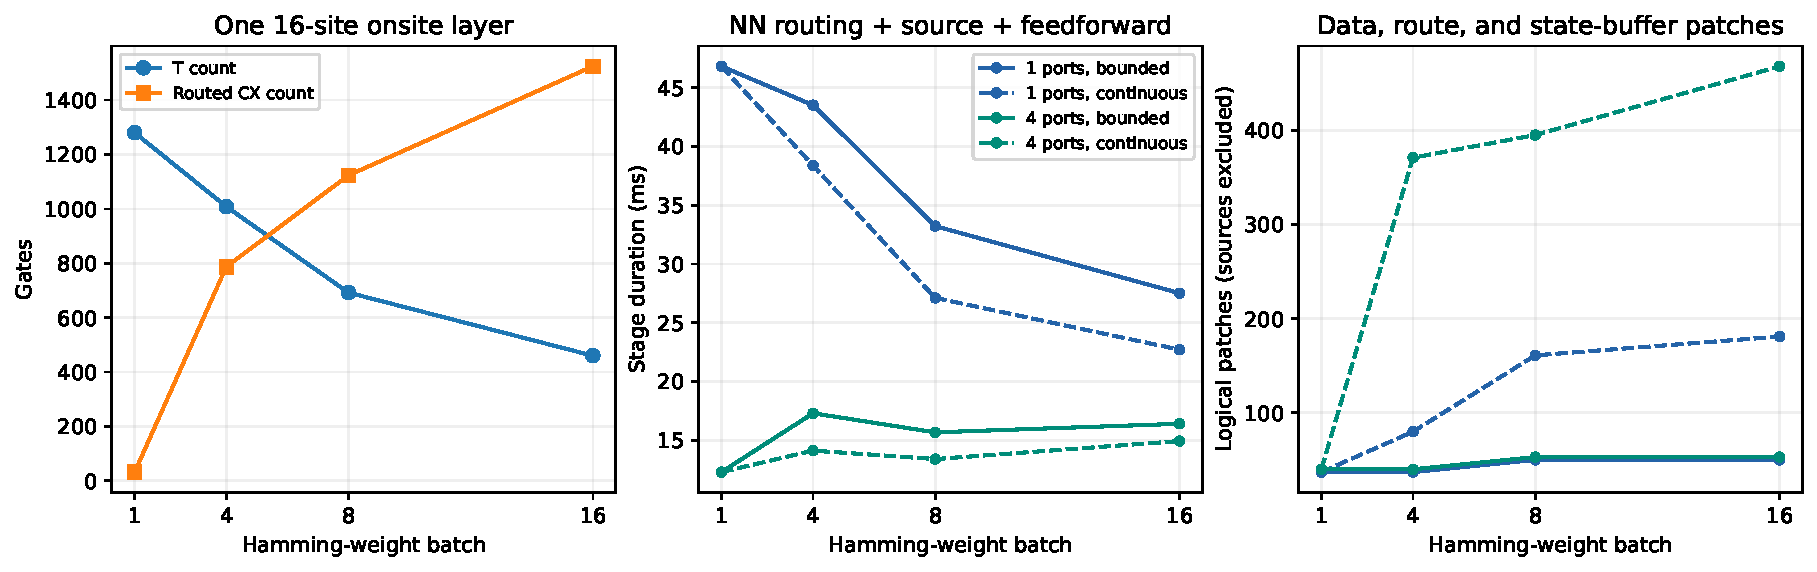
\includegraphics[width=\linewidth]{implementation_ft.pdf}
\caption{One $4\times4$ onsite layer at $\theta=1/36$. Hamming-weight
batching reduces T count but increases arithmetic and routed CX count.
One-state buffers and continuous production distinguish timing from storage
assumptions. The patch count includes packed data/routing and state buffers;
source and surgery footprints are excluded. This constructive schedule
neither optimizes routing nor establishes full-campaign physical area.}
\label{fig:implementation-ft}
\end{figure}

Batch 16 reduces the stage from 1280 to 460 T states, but raises routed
CX count from 32 to 1524. With one source port and bounded storage, the
stage falls from 46.824 to 27.510\,ms. With four ports it instead rises
from 12.282 to 16.398\,ms. Continuous production reduces waiting but can
require hundreds of buffer patches. Thus the aggregate Hamming-weight
resource improvement is supported at the T-count level; its runtime and
area improvement require a better joint routing, arithmetic, and delivery
implementation than is assumed by a count-only comparison.


We then replace abstract delivery by a conservative geometric construction.
A magic state enters at a perimeter output port, moves by adjacent SWAPs
through the patch array, and is consumed next to the target. Reversing the
SWAPs restores every displaced data qubit. Tests verify the complete channel
on entangled data in both injection outcomes. Each SWAP costs three adjacent
CX operations, and the injection takes five logical clocks. The schedule
reserves the traversed patches and their surgery mediators until return.
Embedding patch centers at pitch two and retaining the perimeter gives
225 tiles for batches one and four, or 289 for batches eight and sixteen.
These footprints include gaps and corners; the reference source area is
charged separately, with one bounded output buffer per port.

\begin{figure}[t]
\centering
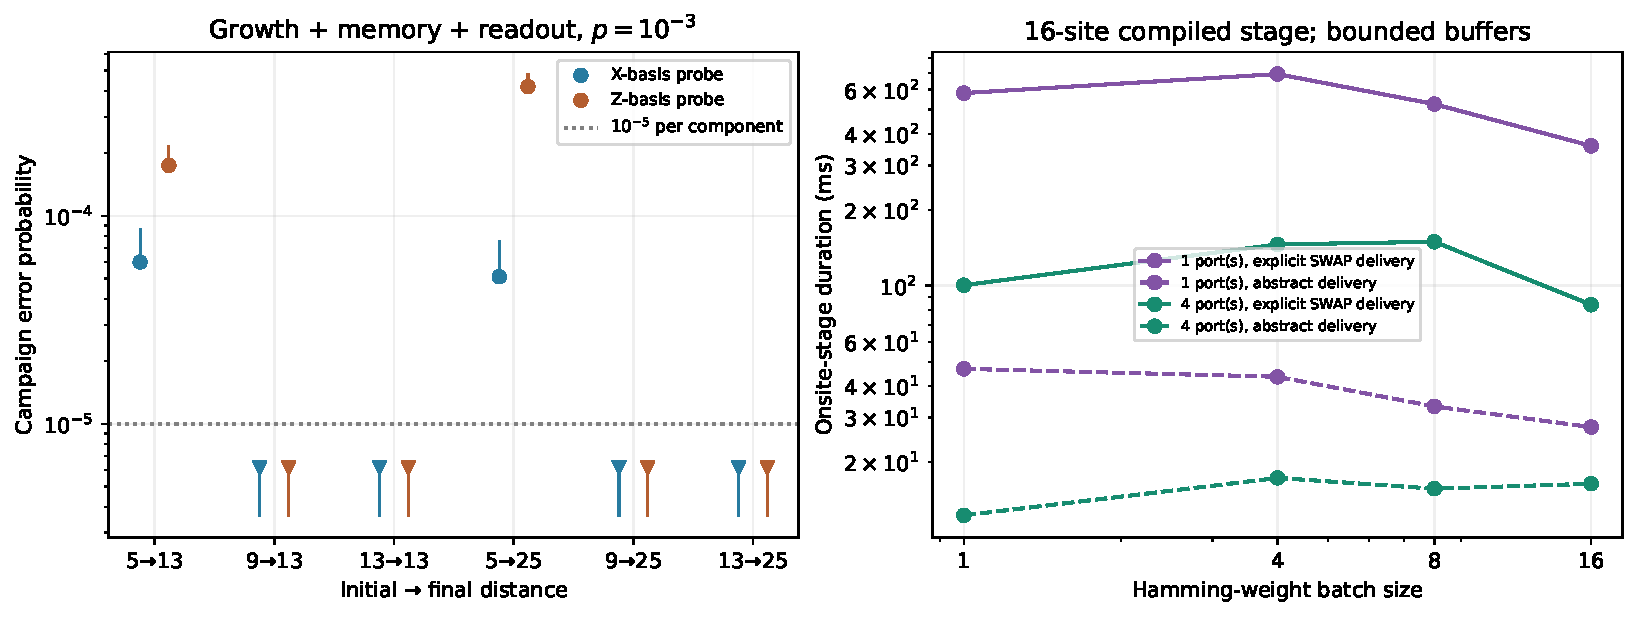
\includegraphics[width=\linewidth]{frontier_components.pdf}
\caption{Larger growth components and geometric FT delivery. Left: one
million shots per basis at $p=10^{-3}$. Circles are measured rates, with segments reaching simultaneous upper
bounds; downward triangles mark upper bounds where no failures were observed.
The experiments include target memory and readout but start from an ideal
encoded state. Right: the same compiled onsite stage with abstract delivery
(dashed) or explicit SWAP transport and restoration (solid). Port count,
state supply, and data routing are held fixed within each pair. The geometric
construction is deliberately conservative and does not establish an optimal
surgery layout.}\label{fig:frontier-components}
\end{figure}

With one port, explicit delivery changes the batch-one and batch-16 stage
times to 581.118 and 358.890\,ms. Four ports reduce these to 100.518 and
84.102\,ms. Batches four and eight can be slower despite using fewer T
states. The ranking is therefore a property of the arithmetic, placement,
and transport together. We retain this isolated stage as a separate layout
scenario rather than extrapolating its transport penalty to every operation
in the capacity plot.

\subsubsection{Locality: the observable and its Trotter error differ}
We compare exact doublon values on nested patches with the same N\'eel
pattern, $U=4$, and observed coordinate $(1,1)$. The smaller patches are
recomputed; completed $4\times3$ and $4\times4$ exact runs supply finite
references. At $\tau=1$, $|D_{3\times3}-D_{4\times4}|=0.04015$ and
$|D_{4\times3}-D_{4\times4}|=0.01488$. Every tested proper subpatch of
$4\times4$ exceeds the 0.0025 spatial allowance at $\tau=1,2$.

\begin{figure}[t]
\centering
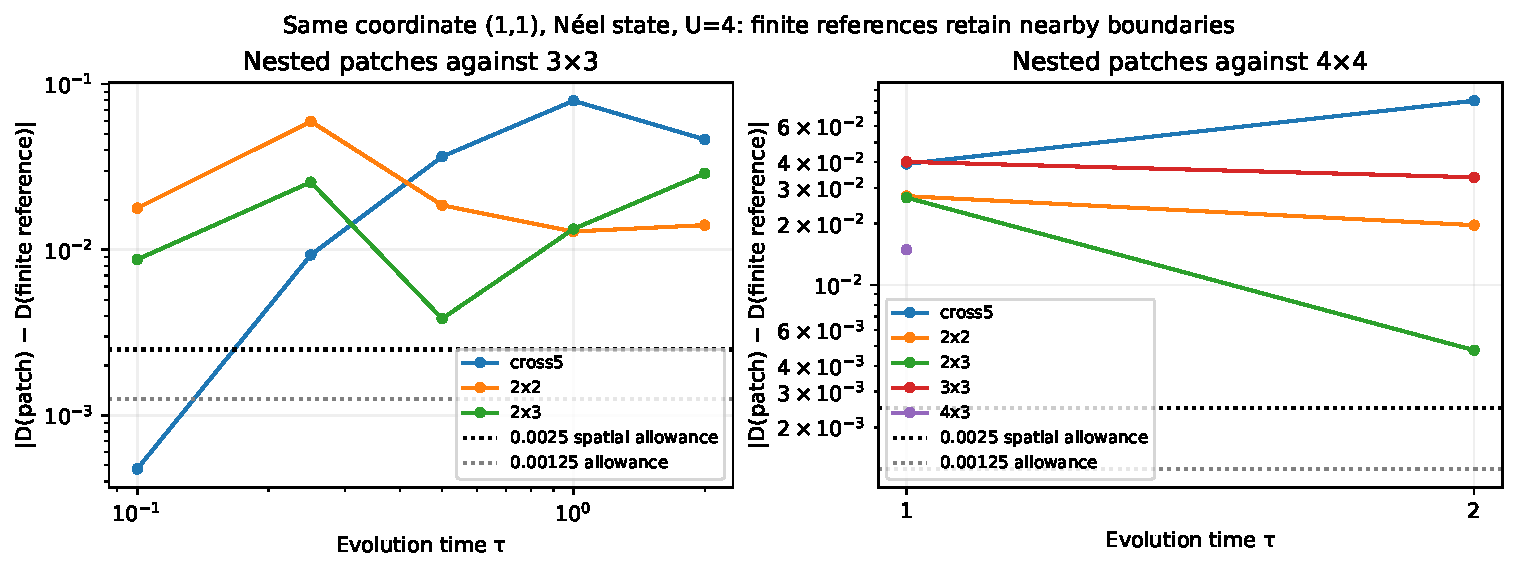
\includegraphics[width=0.94\linewidth]{implementation_locality.pdf}
\caption{Direct nested-patch differences with a fixed observed coordinate.
Each curve compares to the named finite reference. Neither reference
removes the nearby outer boundary, so the data do not certify an infinite
lattice or a saturation length. Agreement of Trotter-error coefficients
must not be used as evidence that these observable differences are small.}
\label{fig:implementation-locality}
\end{figure}

The similar plaquette Trotter coefficients near $\tau=1$ describe the
error of the algorithm relative to each patch's own exact dynamics.
They do not establish convergence of the dynamics themselves. The new
measurements reject the tested aggressive truncations, while leaving a
properly centered larger-patch or independently bounded locality study
as a distinct requirement. At fixed time, a validated local approximation
would also change the task metric: once its patch fits, maximum full-lattice
size no longer measures the cost of that one observable.


A state-independent certificate supplies a complementary sufficient condition.
We center the observable, $O=D-I/2$, so $\|O\|=1/2$, and remove onsite
interactions by a product interaction picture. A two-spin hopping bond has
norm $2J$. The commutator recursion~\cite{nachtergaele2006} and Duhamel's
formula give the deliberately loose bound
\begin{equation}\label{eq:local-certificate}
 \delta_{\rm spatial}(R,\tau)\leq
 \min\left\{1,\frac{2}{7}\sum_{n\geq R+1}\frac{(28|\tau|)^n}{n!}\right\}.
\end{equation}
Here the retained patch contains the graph ball of radius $R$ around the
observed site, and its initial reduced state agrees with the full system.
There are at most four first bonds and seven bonds touching each subsequent
bond. The first omitted boundary crossing needs at least $R+1$ bonds;
Appendix~\ref{app:local-certificate} details the counting.
The geometric tail majorant first meets a 0.0025 allowance at $R=78$ for
$\tau=1$, corresponding to an enclosing $157\times157$ square.
This sufficient radius is not an estimate of the physical light cone.
The bound is too loose to certify the proposed six- or eight-site-wide
patches, while the direct finite-reference checks reject the smallest
truncations. A tight bulk truncation estimate remains separate scientific work.

\begin{figure}[t]
\centering
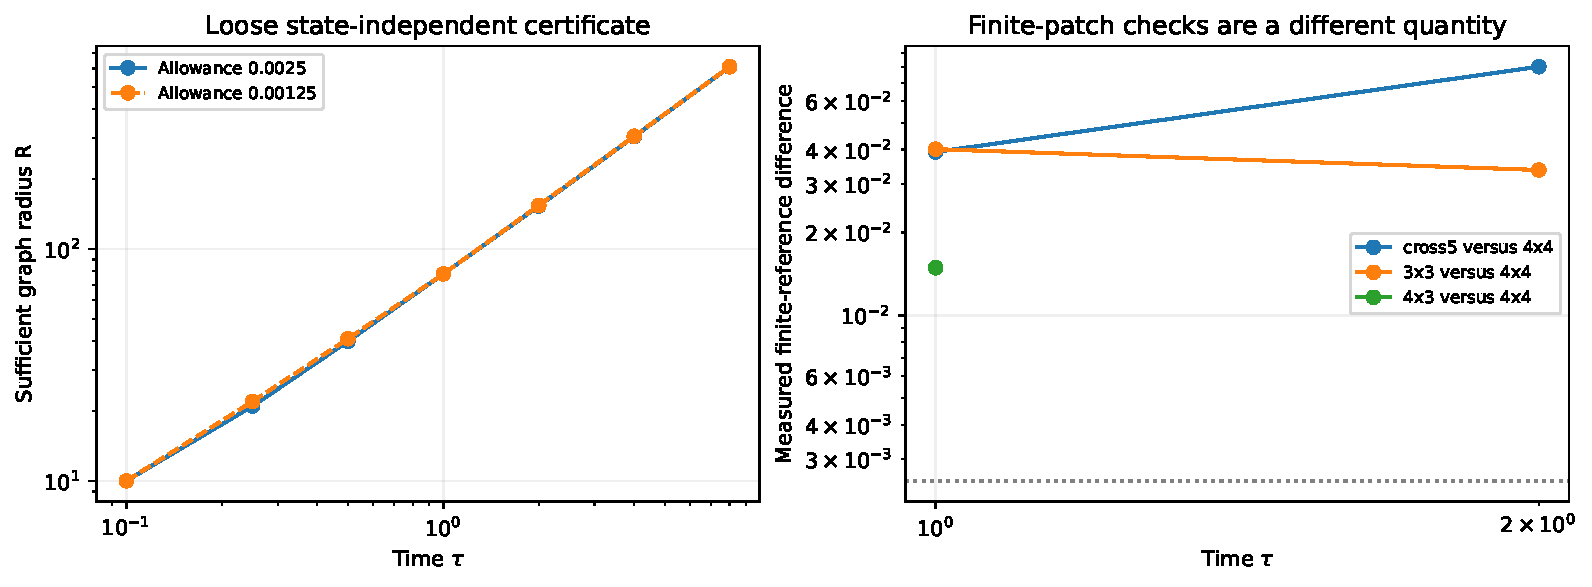
\includegraphics[width=\linewidth]{frontier_locality.pdf}
\caption{Sufficient locality radius from Eq.~\eqref{eq:local-certificate}
(left) and measured finite-reference differences (right). These are different
quantities: a loose uniform bound cannot locate the physical light cone,
and agreement with one finite reference cannot bound its outer boundary.}
\label{fig:frontier-locality}
\end{figure}

\subsubsection{Do the measured costs collapse onto exposure?}
The exposure laws organize the accounting, but a collapse requires an
independently obtained ordinate. We use exact noisy eight-qubit expectations,
held-out affine fits, and enumerated STAR channels rather than plotting an
assumed variance law against its own exponent. For each NISQ circuit,
$\chi_{\rm PEC}$ sums the gate, idle, and SPAM inverse-norm contributions.
The measured variance multiplier divides the estimator variance per attempt
by $D_{\rm ideal}(1-D_{\rm ideal})$; acceptance and fitted slope are included.
Training uncertainty and all six million training shots per fit remain in
the campaign ledger, although the ordinate isolates inference variance.

\begin{figure}[t]
\centering
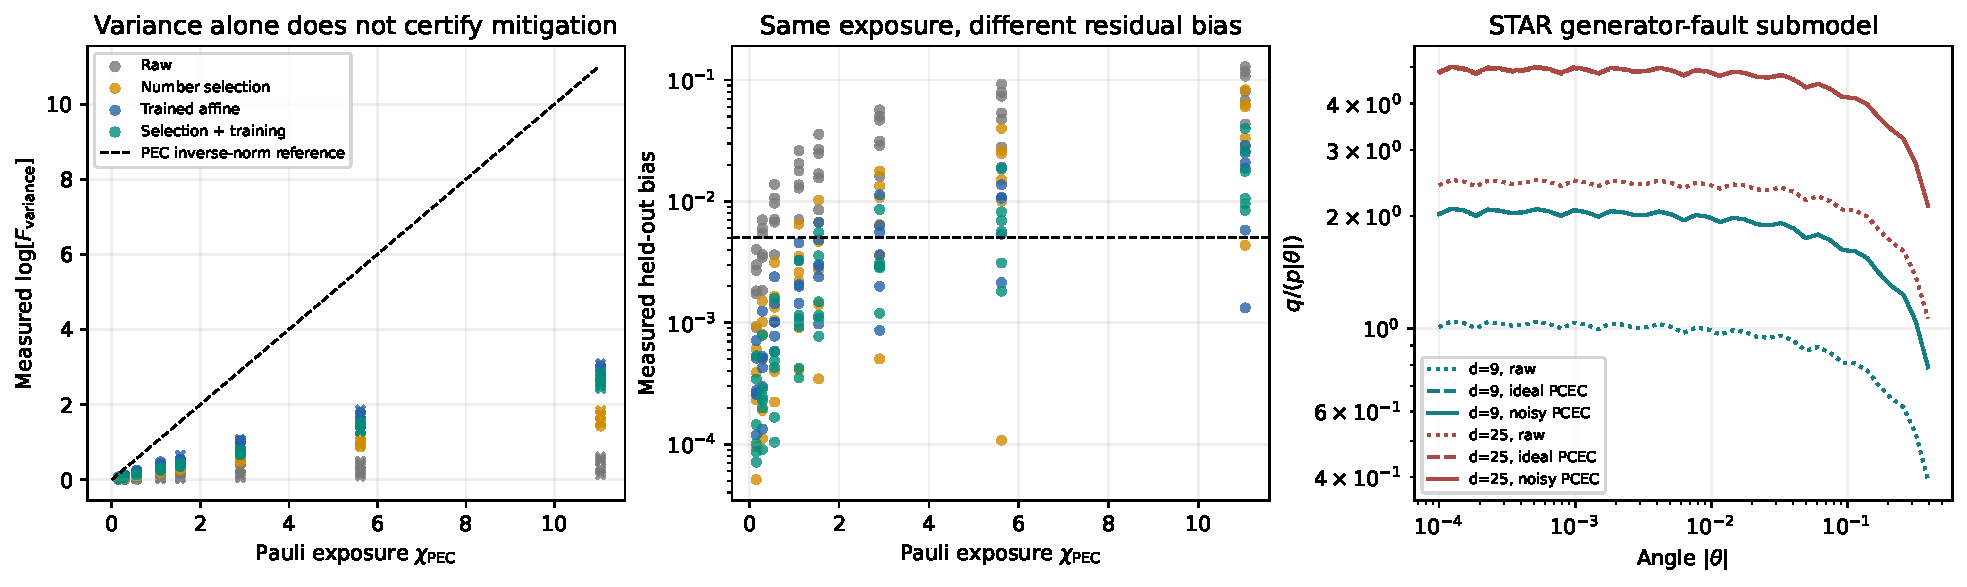
\includegraphics[width=\linewidth]{frontier_exposure.pdf}
\caption{Independent exposure diagnostics. Left and center: matched-noise
held-out tests at $p=10^{-3},10^{-4}$, with crosses marking failure of the
0.005 bias allowance in the left panel. Small variance does not imply small
bias. The dashed diagonal is the separate whole-circuit PEC inverse-norm
reference. Right: $q/(p|\theta|)$ from the exact generator-fault submodel at
$p=10^{-3}$, separating raw, ideal-PCEC, and noisy-PCEC channels. Generic extraction faults and
growth are absent from these channel curves.}\label{fig:frontier-exposure}
\end{figure}

The trained estimators have much smaller variance than the PEC reference,
but some fail the held-out bias requirement at the same exposure. These
data do not support a universal variance-and-bias collapse onto one scalar.
Likewise, STAR's normalized error depends on the correction channel and
injection distance. The useful outcome is a test of the law's domain:
exposure alone is insufficient to certify an estimator or a full injection
protocol.

\subsection{Reconciliation of the workshop calculations}\label{sec:reconciliation}
We evaluate the two supplied workshop implementations at $4\times4$,
$\tau=1,2$, and $0.01$ absolute error, with common elementary clocks and
a common Gaussian doublon shot budget. The statistical allowance is 0.004
at $D_\star=0.1$, giving 21,609 ideal shots. Taking 25\% of the error
budget for the larger of our two planning coefficients gives 11 and
23 steps. This step convention isolates resource differences; it is not
an accuracy certificate for the different observables and unspecified
circuits underlying the supplied models. We remove the IQUS physical-cone
discount and explicitly fix its signal scale. The original implementations
remain untouched, and their imported Python sources are preserved alongside
the comparison data.

Matching these settings does not make the resource inventories identical.
At $\tau=1,r=11$, the two-qubit gate counts are approximately 4,750,
3,520, and 2,640 for our native proxy, Martin, and IQUS, respectively.
The corresponding STAR rotation counts are 2,443, 2,288, and 880.
Their STAR shot times are approximately 50.3, 1.86, and 0.686 ms,
reflecting different rotation parallelism and retry schedules even after
the syndrome clock is matched. Native factory and logical-error conventions
also remain different. These outputs diagnose assumptions rather than
rank three fully specified machines.

An additional comparison applies every injection law to the identical
ledger $R=2{,}443$, $\Theta=64$ at $p=10^{-3}$. Martin's native
attenuation convention gives $\chi=0.9772$, the IQUS count convention
gives 2.6042, the exact original-injection inverse gives 2.6066, and
the angle-plus-floor law gives 0.4817. Thus even the phrase ``count law''
does not identify a common estimator convention. The differences do not
collapse onto precision, evolution time, syndrome clock, and one injection
switch alone: compilation, delivery, and the estimator must also be named.
This shared-ledger calculation is an algebra check, not an empirical
collapse test or independent evidence for a mitigation law.

\subsection{Back-of-the-envelope+ discussion example}\label{sec:discussion}
We use simple analytical laws to expose the architectural tradeoffs, with
$p=10^{-3}$, $10$ ns gates, $100$ ns measurement/reset, $240$ ns syndrome
cycles, $U/J=4$, and a one-week budget $B$. The original reference below
emphasizes $\eps=0.001$; both precisions remain explicit in the current
comparison of Section~\ref{sec:physics-sweep}. We compare NISQ, STAR, FTQC,
and the hybrid using a common total-error target. Each arm can choose its
error allocation, step count, and resource-state supply within the declared
search. This removes a fixed allocation that previously forced unnecessary
cleanup at the strict $4\times4$ FT point.
The current finite-patch capacity sensitivity is shown in
Figure~\ref{fig:patch-capacity}, and the directly checked $4\times4$
allocations in Table~\ref{M-tab:direct-budgets}. We first develop the common
model using the original $3\times3$ reference, retaining its longer-time
and $\tau=L/4$ scenarios for comparison.

\paragraph{Ordering-specific time dependence.}
We extend exact fixed-sector calculations on $2\times2$ and $3\times3$
patches through $\tau=8$, and check the two product formulas separately.
The termwise evolution retains the ordering of the compiled Pauli circuit;
the plaquette evolution retains its onsite/pink/gold splitting. Independent
small-system comparisons check the factorized sector implementation against
the qubit circuits and the sparse Hamiltonian evolution.

For each ordering $\mathcal A$ and measured time, we increase $r$ until the
last two estimates of $|D_r-D_{\mathrm{exact}}|r^2$ agree within $5\%$.
The observed $r^{-2}$ dependence survives, but its coefficient is neither a
single power of time nor independent of the ordering. On $3\times3$, the
plaquette and termwise coefficients are respectively $0.218$ and $0.0767$
at $\tau=1$, and $7.67$ and $23.74$ at $\tau=8$.
Figure~\ref{fig:time-coefficients} shows the full time dependence and patch
sensitivity. At $\tau=2$, the $4\times3$ plaquette and termwise
coefficients are $1.136$ and $0.702$, compared with $0.926$ and $0.381$
on $3\times3$. At $\tau=4$ they are $4.100$ and $2.728$, compared with
$5.270$ and $1.957$. These differences preclude a claim of bulk convergence.

At the smaller step counts admitted by the optimizer, higher-order terms
can matter. We therefore also measure $r=\lceil8\tau\rceil$ and twice that
value on $3\times3$. The coefficient used below is the largest sampled
value across these finite-step checks and the asymptotic pair. This corrects
an underestimate caught by direct validation at loose precision.

For the planning curves we use
\begin{equation}\label{eq:discussion-r}
 C_{\mathcal A}^{\mathrm{plan}}(\tau)
 =1.1\max_{s\leq\tau,\ s\in\mathcal T}
 C_{\mathcal A}^{3\times3}(s),\qquad
 \eps_T(r,\tau)=\frac{C_{\mathcal A}^{\mathrm{plan}}(\tau)}{r^2},
\end{equation}
where $\mathcal T$ is the measured time grid. The running maximum avoids
relying on isolated small-patch cancellations; it is a planning choice for
the final-time observable, not a change to a whole-curve accuracy target.
The $10\%$ margin is a declared sensitivity, not a finite-size error bound.
We retain pointwise-coefficient costs separately. No time power is fitted,
and we do not extrapolate beyond $\tau=8$. The $2\times2$ resource point
uses its own measured coefficients; other sizes transfer the $3\times3$
reference. The $\tau=L/4$ panel therefore
stops at $L=32$. Transfer to larger lattices remains an assumption.

\begin{figure}[t]
\centering
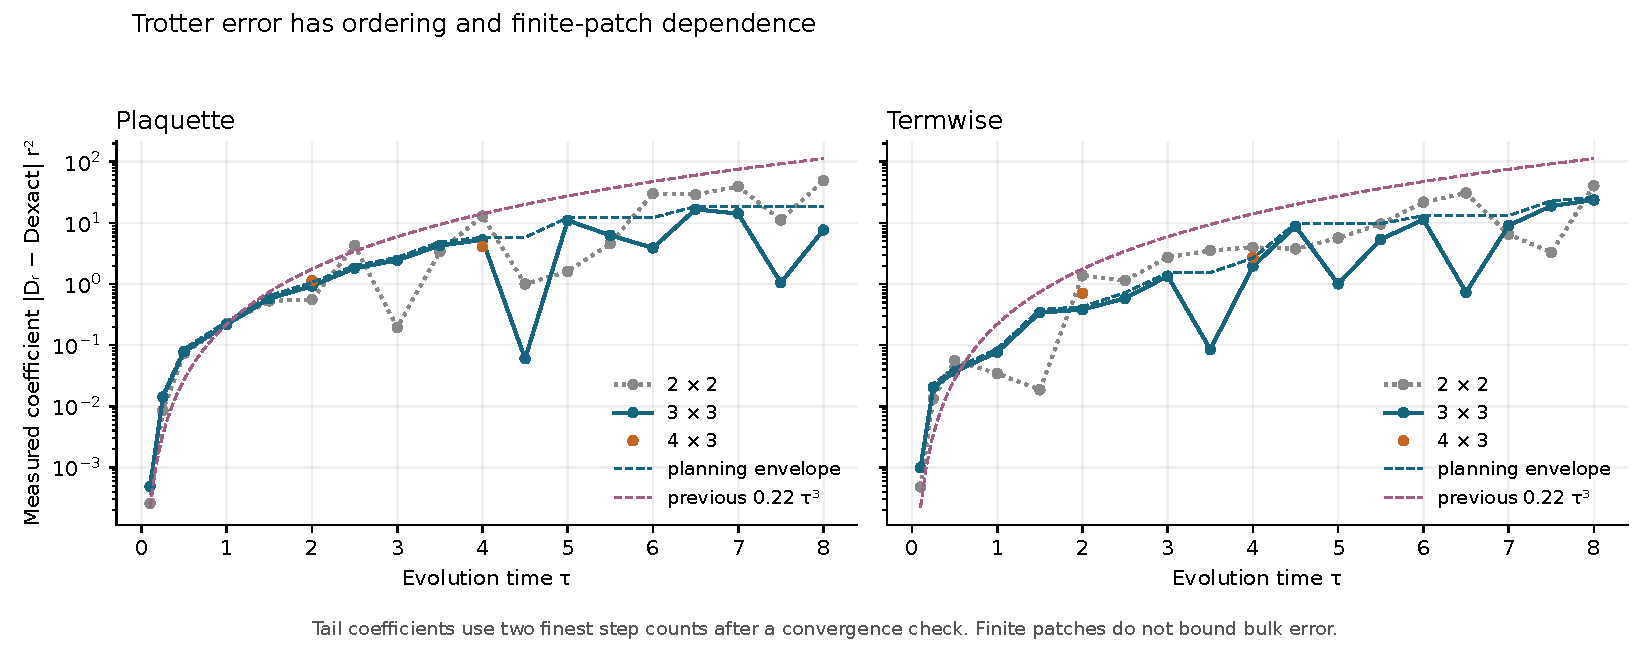
\includegraphics[width=\linewidth]{time_calibration.pdf}
\caption{Local Trotter-error coefficients depend on time, ordering, and
patch. Each point uses the finer pair after a step-convergence check.
The dashed blue curve is the planning envelope in
Eq.~\eqref{eq:discussion-r}; the previous $0.22\tau^3$ prescription is
shown for comparison. The patch differences are not a bulk error bound.}
\label{fig:time-coefficients}
\end{figure}

\paragraph{Joint error allocation.}
For each candidate we impose
\begin{equation}\label{eq:optimized-budget}
 \eps_{\mathrm{stat}}=\eps-\eps_T-\eps_L-\eps_{\mathrm{syn}}
       -\Gamma N_Tq_T-\eps_{\mathrm{res}}>0.
\end{equation}
Unused components vanish: termwise STAR has no synthesized rotations or
supplied T states, and the hybrid synthesizes no variable rotations.
The logical reserve satisfies $\Gamma V_Lp_L(d)\leq\eps_L$.
Mitigated arms reserve $\eps_{\mathrm{res}}=0.1\eps$ for residual estimator
bias, including channel mismatch and unmodeled SPAM. Its affordability is
assumed. FT has no mitigation reserve; its modeled faults are charged to the
logical and magic-state terms.

We search Trotter allowances, logical reserves, synthesis tolerances, and
integer-step neighbors, with $r\geq\lceil8\tau\rceil$ as a small-step guard.
FT and hybrid independently compare raw cultivated states with one cleanup
stage and optimize $1$--$16$ sources. Both use the same source menu.
The result is the best candidate in the declared search, not a global
optimum over protocols or source-quality/throughput tradeoffs.
The resulting per-arm allocations are recorded with each resource point.

For effective mitigation and encoded planning curves,
\begin{equation}
 M_0=\left\lceil\frac{1.96^2D_*(1-D_*)}{\eps_{\mathrm{stat}}^2}\right\rceil,
 \qquad Q_{\mathrm{week}}=q\max\left(1,
 \left\lceil\frac{M_0Ft_{\mathrm{shot}}}{B}\right\rceil\right),
 \qquad D_*=0.1.
\end{equation}
The PEC references retain the sufficient Hoeffding count from
Eq.~\eqref{eq:shots}. Distance follows the common surface-code fit, with
worst-case $\Gamma=\sqrt F$ amplification for mitigated logical and magic
faults. The central delivery model has four effective parallel lanes;
these are a throughput assumption, not a compiled dependency schedule.

\paragraph{The per-arm laws.}
NISQ uses the Willow circuit-count anchor~\cite{phasecraftwillow2025},
\begin{equation}
 G_2=4372\frac r3\left(\frac L6\right)^3,\qquad
 D_{\mathrm{circ}}=294\frac r3\frac L6,\qquad
 \log F_{\mathrm{eff}}=\log(\eta_*)\frac p{10^{-3}}\frac{G_2}{4372}.
\end{equation}
The central $\eta_*=100$, with $10$--$1000$ sensitivity, is an assumed
sampling overhead, not a fit to experimental accuracy. Its bias reserve
also remains uncalibrated. Two explicit PEC comparisons use two-qubit
inverse-channel exposure, $\log F\simeq4pG_2$, or the saved compiled
full-noise exposure with bulk terms proportional to $r$ and separate SPAM.
The NISQ proxy transfers the plaquette error coefficient without asserting
a match to the experimental ordering.

Termwise STAR uses
\begin{equation}
 \Theta=(5L^2-4L)\tau,\qquad R=[16L(L-1)+2L^2-2]r+1,
 \qquad \log F_{\mathrm{STAR}}=4\alpha p\Theta+4fR,
\end{equation}
with $\alpha=1.5$, $f=10^{-5}$, and $18$ code clocks per completed
rotation~\cite{akahoshi,toshio}. The scenario range varies $f$ from zero to
$10^{-4}$ and lanes from eight to one. Refinement leaves the angle term
unchanged while increasing the floor term and execution time.
FT uses plaquette counts, logarithmic synthesis, and $F=1$.
The hybrid uses the same plaquette workload, injecting variable rotations
and supplying fixed T states. It therefore has exponent
$4\alpha p\Theta_{\mathrm{dyn}}+4fR_{\mathrm{dyn}}$.

FT and hybrid share the rounded cultivation reference: $1024$ source
qubits, $100$ syndrome cycles per state plus $2d$ handoff cycles, and raw
state error $2\times10^{-9}$~\cite{gidney2024cultivation}. The optional
$15$-to-$1$ cleanup changes source error, footprint, and service together.
Supply overlaps consumption; the reference charges nine code clocks per T
and varies source service time by $0.5$--$4$. These source models remain
conditional implementations. Termwise STAR already avoids fixed T gates,
so a hybrid advantage is algorithm-dependent.

\begin{figure}[t]
\centering
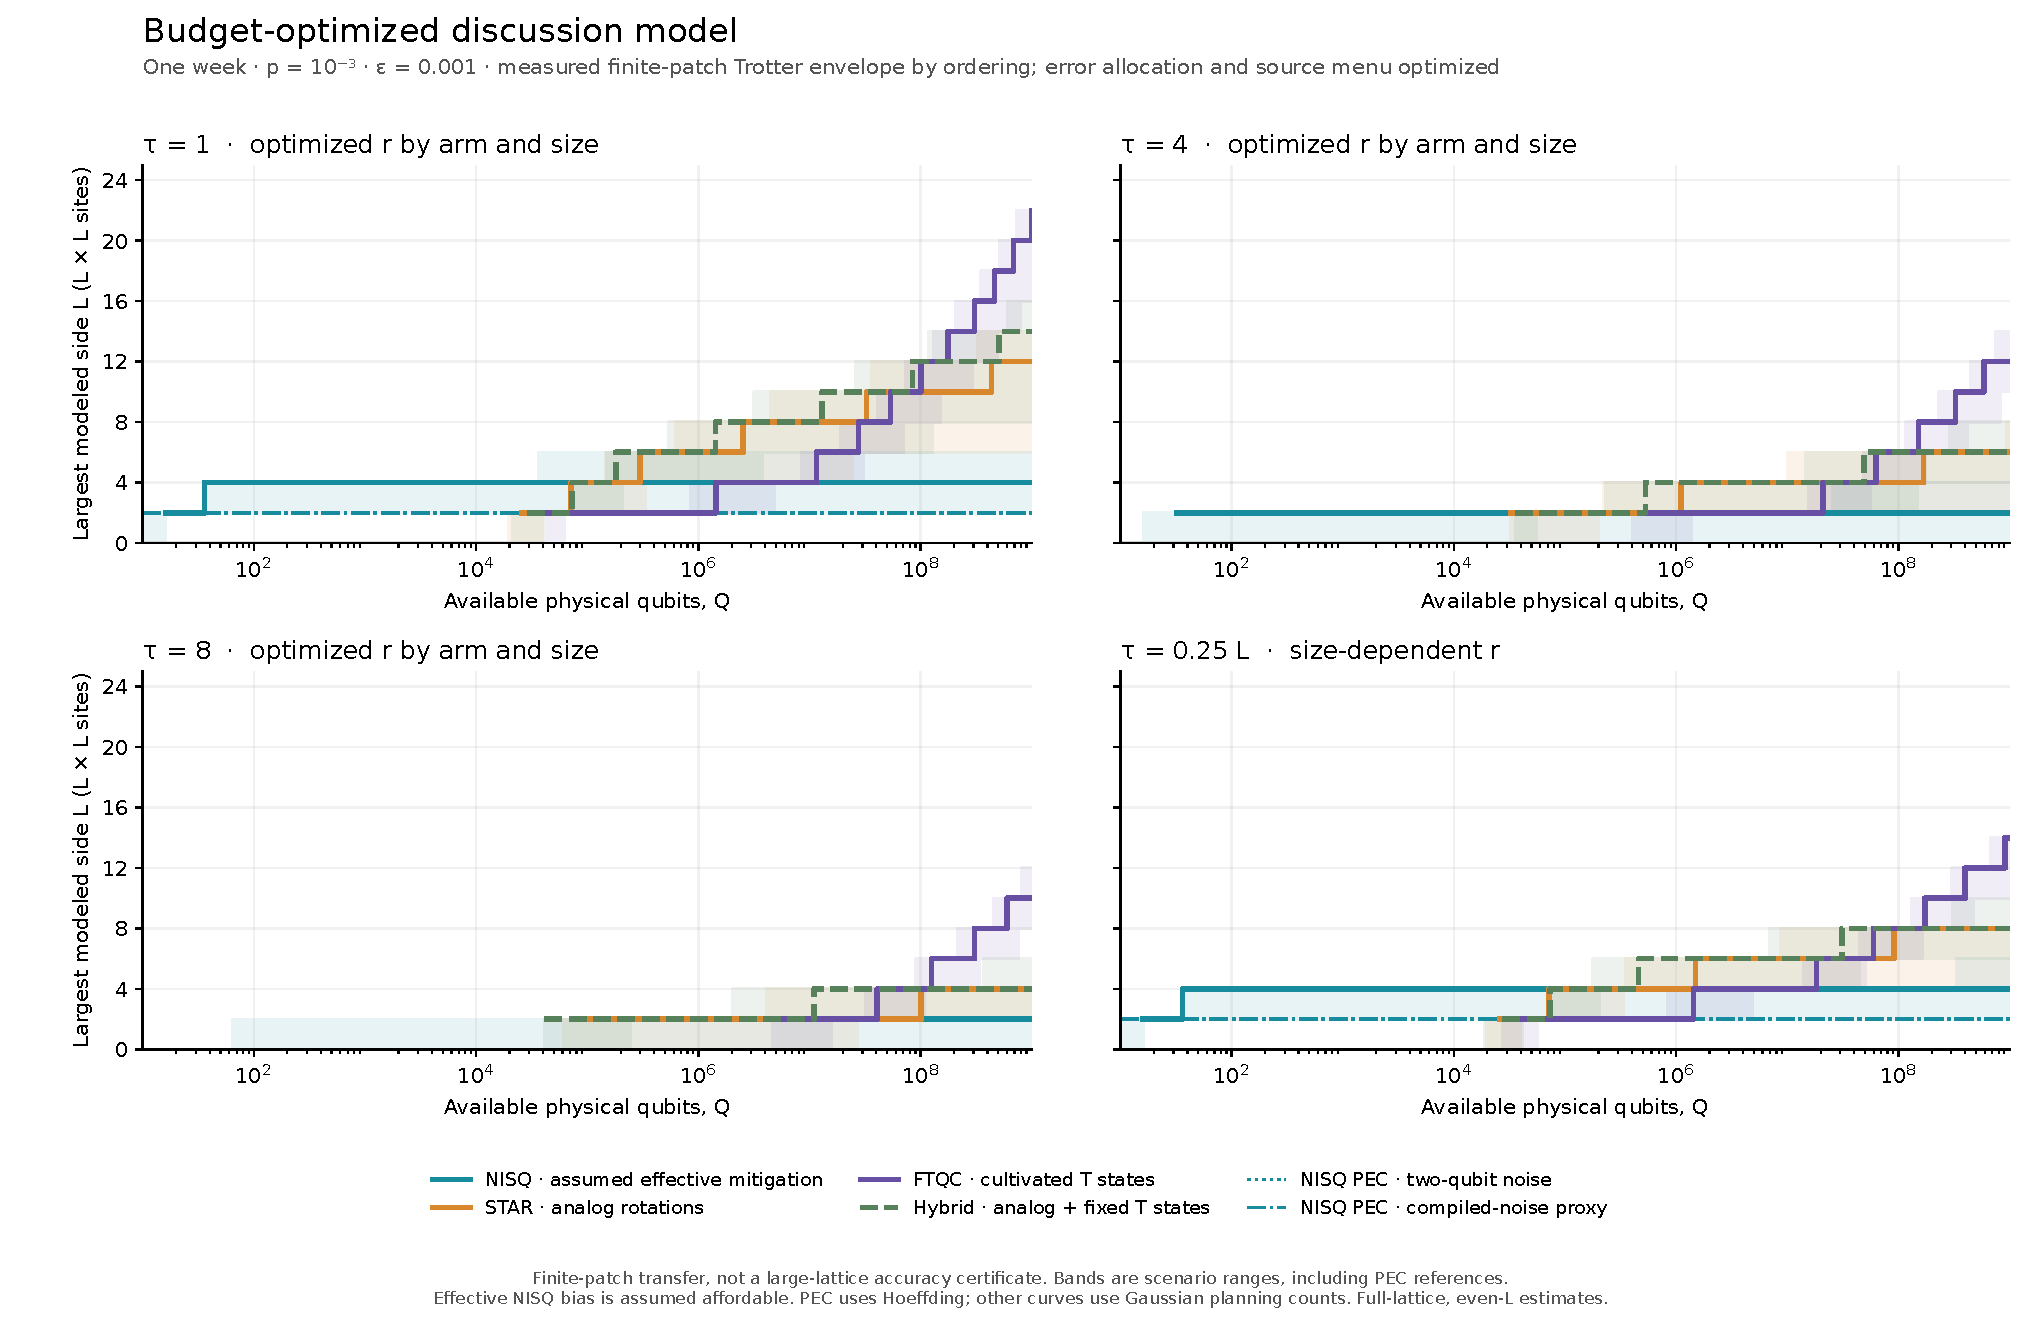
\includegraphics[width=\linewidth]{discussion_capacity.pdf}
\caption{Budget-optimized discussion comparison at $\eps=0.001$.
Each arm selects its error allocation and step count using the measured
finite-patch planning envelope. Lines are central assumptions; bands span
delivery and mitigation scenarios, including NISQ PEC references. They do
not represent uncertainty in bulk Trotter error. The fourth panel follows
$\tau=L/4$. Full lattices and even $L$ are modeled. Effective NISQ mitigation
is an assumed estimator scenario, not a demonstrated accuracy result.}
\label{fig:discussion}
\end{figure}

Using the $3\times3$ planning reference at $\tau=1$, the central areas are
\begin{center}
\small
\begin{tabular}{rrrrrr}
\toprule
Lattice & $\eps$ & NISQ effective & STAR & Hybrid & FTQC\\
\midrule
$4\times4$ & $.001$ & $36$ & $71442$ & $73348$ & $1.43\times10^6$\\
$4\times4$ & $.01$ & $36$ & $46818$ & $48420$ & $61974$\\
$6\times6$ & $.001$ & $3.64\times10^{10}$ & $298356$ & $180798$ & $1.16\times10^7$\\
$6\times6$ & $.01$ & $81$ & $101802$ & $103548$ & $126268$\\
\bottomrule
\end{tabular}
\end{center}
For strict $4\times4$ FT, the selected $r=31$ candidate allocates about
$33.6\%$ to statistics, $25.3\%$ to Trotter error, $36.2\%$ to magic-state
error, $2\%$ to logical faults, and $3\%$ to synthesis. Cleanup is no longer
needed, reducing the previous $5.66$ million-qubit estimate by about a
factor of four. The strict $6\times6$ FT candidate still chooses cleanup.
The hybrid improves on termwise STAR at strict $6\times6$, but not at
$4\times4$. NISQ's effective estimate remains conditional on the specified
sampling multiplier and affordable residual bias; its PEC alternatives are
shown alongside it.

We separate the changes with an ablation that first optimizes the budget
under the old cubic-time coefficient and then replaces that coefficient.
A finer allocation grid improves the selected $\tau=1$ costs by at most
$18\%$. Direct checks at the optimized step counts fit the planning
envelope on $3\times3$. At strict $4\times4$, $\tau=8$, the optimized
STAR floor exposure is $2.28$, below its angle exposure $3.07$; the earlier
floor-dominated example depended on the assumed cubic time law. Neither validates
the transfer from finite patches to large lattices. The earlier four-step
compiled reference and fixed-allocation discussion results are retained as
historical comparisons. The remainder develops their resource laws and
implementation evidence.

\section{Earlier reference models}\label{sup:models}
\subsection{STAR: angle exposure, floors, and delivery}

For independent residual dephasing $q_j$ after completed rotations,
\begin{equation}\label{eq:star-v0}
 \Gamma^2=\prod_j(1-2q_j)^{-2},\qquad
 \chi_{\mathrm{STAR}}=-2\sum_j\log(1-2q_j)\simeq4\sum_jq_j.
\end{equation}
Original STAR uses the post-RUS reference $q_0=4p/15$~\cite{akahoshi}.
The small-angle reference uses $q_j=\alpha p|\theta_j|+f$, with
$\alpha=1.5$ in our angle convention and a declared floor $f=10^{-5}$~\cite{toshio,chung}. The floor is a sensitivity motivated by injection and
growth, not a measured error floor at this operating point. Fixed $\pi/8$
rotations retain $q_0$; we do not extrapolate the small-angle fit to them.
Consequently,
\begin{equation}\label{eq:star-exposure}
 \chi_{\mathrm{STAR}}\simeq4\alpha p\Theta_{\mathrm{dyn}}+4fR
                     +\frac{16p}{15}T_{\mathrm{fixed}}.
\end{equation}
The implementation evaluates the logarithmic product in Eq.~\eqref{eq:star-v0};
the physical channel models themselves remain approximations. Their three
exposures have different responses to compilation and refinement. In
particular, $fR\sim\alpha p\Theta_{\mathrm{dyn}}$ marks a floor/angle
competition, while repeated basis changes can dominate separately.

The serial reference allocates
$n_{\mathrm{data}}=\lceil1.5(2N+6)\rceil$ tiles and six injection tiles.
It charges $18$ code clocks per rotation, with one clock equal to $d$
syndrome cycles, plus startup, readout, and feedforward. This is a delivery
model. A small-angle error law does not itself establish its acceptance,
throughput, or footprint. The explicit retry refinement below adds both
parallelism and its area cost.

\subsection{Physical computation: gates, locality, and idle exposure}
For a $k$-qubit depolarizing location with total nonidentity-Pauli probability
$p_k$, set $s_k=1-4^kp_k/(4^k-1)$. The inverse has identity coefficient
$1+p_k/s_k$ and $4^k-1$ coefficients $-p_k/[(4^k-1)s_k]$, giving
\begin{equation}\label{eq:physical}
 \gamma_k=1+2p_k/s_k,\qquad
 \chi_{\mathrm{phys}}=\sum_{\ell\in\mathrm{cone}}2\log\gamma_{k_\ell}
 \simeq4pG_2+4(p/10)G_1+4p_{\mathrm{idle}}G_{\mathrm{idle}}+\chi_{\mathrm{SPAM}}.
\end{equation}
Preparation and readout bit flips use $\gamma=1/(1-2p)$. The continuous-time
idle convention composes as
\begin{equation}
 p_{\mathrm{idle}}(\Delta t)=\frac34
 \left[1-(1-4p/3)^{\Delta t/(100\,\mathrm{ns})}\right].
\end{equation}
Only channels in the compiled measurement's backward dependency cone enter
the local PEC product. CPTP channels outside that cone cannot affect its
expectation. This sufficient cone can still exceed the observable support
needed at a specified tolerance.

\subsubsection{Fermionic blocks and parallel motion}
Two-mode hopping, density evolution, and fermionic Hadamards are extracted
from the plaquette workload while preserving its noncommuting stage order.
A number-conserving Gaussian gate has odd-sector matrix $G\in U(2)$,
vacuum amplitude one, and double-occupation amplitude $\det G$. An Euler
decomposition of $G$ therefore compiles to local $Z$ rotations and at most
two native $R_{ZZ}$ gates. In particular,
\begin{equation}
 V(\theta)=e^{-i\theta(XX+YY)},\qquad
 F_{\mathrm{swap}}=(S\otimes S)V(\pi/4),
\end{equation}
so a swap followed by hopping can fuse into the same pair of entanglers with
a changed angle. Products of Gaussian gates on the same adjacent pair fuse
through operations on disjoint wires. A commuting density rotation adds at
most one entangler.

The compiler gathers independent plaquette groups into intervals of a live
fermionic order using parallel odd-even transposition sorting. All swaps are
adjacent physical fermionic swaps on a snake embedded in the square grid~\cite{kivlichan2018}. It then executes disjoint groups concurrently and tries
six initial-order/local-route choices. A preparation permutation is free for
the specified occupation product state, while the final wire map and Fock
signs remain explicit. Using only snake edges leaves room for a better
two-dimensional compiler. The trapped-ion experiment's all-to-all connectivity
and free ordinary-SWAP relabeling are a different compilation assumption~\cite{alam2025}.

The first onsite stage is a scalar on the initial Fock state, and the last
onsite stage commutes with the measured doublon. Removing them is exact for
this task. A reverse traversal through even fermionic blocks then removes
blocks on disjoint support. These reductions are available to every arm;
the current encoded resource curves retain the original full logical workload.

\begin{center}
\begin{tabular}{lrrr}
\toprule
$L=4,\ \tau=1,\ r=4$ & Entanglers & $10$ ns layers & Local $\chi$\\
\midrule
Greedy fused route with cone & $3149$ & $2187$ & $35.297$\\
Parallel route, full evolution & $3204$ & $1074$ & $22.214$\\
Parallel route with observable reductions & $2648$ & $964$ & $20.017$\\
\bottomrule
\end{tabular}
\end{center}
The final row has $t_a=9.84~\mu\mathrm{s}$ and exposure
\begin{equation}
 \chi=10.5927_{2q}+4.1201_{1q}+5.1681_{\mathrm{idle}}+0.1361_{\mathrm{SPAM}}.
\end{equation}
Its strict-precision threshold is $Q_{\min}\simeq2.13\times10^6$, versus
$12168$ with zero idle on the same circuit. Idle has decreased substantially
but remains material. The gain combines scheduling, placement, fusion, and
observable algebra; zero idle is a sensitivity rather than a demonstrated
alternate schedule.

\subsubsection{What the million-qubit estimate means}
The $4\times4$ circuit occupies $32$ active qubits, packed into a $36$-qubit
square. At the strict precision, the reference assigns
$\Gamma^2=e^{20.017}\simeq4.94\times10^8$ and a sufficient budget of
$N_0\Gamma^2\simeq3.64\times10^{15}$ shots. At $9.84~\mu\mathrm{s}$ per
attempt, this requires $59239$ copies to fit within one week, giving
$Q_{\min}=2132604$. The large area is entirely a sampling-throughput cost.
For the same circuit, duration, and precision, removing idle noise gives
$Q_{\min}=12168$; retaining only two-qubit noise gives $Q_{\min}=180$.
These are noise ablations, not demonstrated improvements or alternative
predictions for the declared device.

Experiments require an additional calibration of the NISQ model.
Phasecraft and Quantinuum simulated a $7\times4$ lattice with $56$ qubits,
using training with fermionic linear optics (TFLO) and time-series
smoothing~\cite{alam2025}. The Willow study reached $6\times6$ with $72$
fermionic-mode qubits, using TFLO, symmetry selection, and other
application-specific processing~\cite{phasecraftwillow2025}. Our gatewise
PEC bound does not describe these estimators. Nor do those demonstrations
establish our particular $0.001$ absolute-error contract at every
interacting data point. Their compilation is also a relevant benchmark:
Willow's published $4\times4$ formula gives $1620$ CZ gates at four steps,
where our reference uses $2648$ native $R_{ZZ}$ gates. This comparison needs
the respective gate implementations and schedules, not only a gate-count
ratio. We therefore retain the current curve as a specified PEC reference;
the resource frontier for experimentally informed physical estimators
remains unestablished.

\subsubsection{Exact circuit cones and physical truncation}
For the original plaquette block ordering, the sufficient interior cones
checked at $r=1,2,4$ contain $(4r+2)^2=36,100,324$ sites. The $r=1$
circuits at $L=8,12,16,20$ all compile to $2001$ native entanglers on $72$
modes in that implementation. Ordered termwise sweeps can instead have
global strict dependencies even at one step. Neither observation establishes
the smallest Hamiltonian region needed at finite tolerance.

At fixed evolution time a local-observable truncation may eventually remove
size dependence, whereas a time family such as $\tau\propto L$ probes
growing physical reach. A truncation must receive a bias allowance in
Eq.~\eqref{M-eq:budget}; it cannot be inferred solely from the strict circuit
cone. Section~\ref{sec:calibration} begins the finite-patch check and states
what its outer boundary leaves unresolved.


\subsection{Full fault tolerance and the hybrid}
For $R$ synthesized rotations each with operator error $\zeta$, telescoping
unitaries bound the observable bias by $2R\zeta$. We set
$\zeta=\eps_{\mathrm{syn}}/(2R)$. The deterministic synthesis fit
\begin{equation}
 T_R=\left\lceil3.02\log_2(1/\zeta)+0.77\right\rceil,\qquad
 N_T=T_{\mathrm{fixed}}+RT_R,
\end{equation}
has the expected logarithmic scaling~\cite{ross}. At the compiled points,
actual CUDA-Q GridSynth words replace this estimate. At $L=4,\tau=1,r=4$, termwise Strang has $889$ variable rotations,
no fixed T gates, and $61178$ synthesized T gates. Plaquettes have $288$
variable rotations and $576$ fixed T gates, for $19584$ synthesized T gates:
$66$ per variable rotation. Independent matrix reconstruction checks the
precision of every distinct emitted word. Whole-program synthesis at
$L=2,4$ agrees with the class-weighted counts; $L=6,8$ use those counts
before inter-gate optimization.

\subsubsection{Conventional factory reference}
Injected-state error $p_{\mathrm{in}}$ is separate from gate error $p$.
The current conventional reference uses $46p/15$, with alternatives retained
as sensitivities; this coefficient is not calibrated to our asymmetric
$p_{1q}=p/10$ noise model. For a 15-to-1 stage~\cite{litinski},
\begin{equation}
 a_1=1-15p_{\mathrm{in}},\quad q_1=35p_{\mathrm{in}}^3,\quad
 q_2=35q_1^3.
\end{equation}
One stage reserves twelve tiles, including its output, and takes $11/a_1$
mean code clocks. The deliberately serial two-stage reference reserves
two eleven-tile blocks and fifteen storage tiles, so
\begin{equation}
 n_F=37,\qquad c_F=\frac{15(11/a_1)+11}{1-15q_1}.
\end{equation}
Both stages use the selected code distance, and protected factory faults
enter $V_L$. Correlations, transport, and rejection-tail latency are not
resolved by this leading-order mean-service model.

For $F$ factory copies, the FT timing reference is
\begin{align}
 C_{\mathrm{FT}}&=2+\max(9N_T+2R,\lceil N_T/F\rceil c_F),\\
 t_a&=C_{\mathrm{FT}}dt_c+N_Tt_{\mathrm{ff}}+t_{\mathrm{reset}}+t_{\mathrm{meas}},\\
 q_a&=2d^2(n_{\mathrm{data}}+Fn_F).
\end{align}
Nine clocks per T is the compact-block consumption reference~\cite{litinski};
the $2R$ term is an extra Clifford-work placeholder. We optimize $F$ over
$\{1,2,4,8,16\}$ together with level and distance, subject to
$N_Tq_{1,2}\leq\eps_{\mathrm{magic}}$. Supply and consumption must be varied
together: speeding consumption alone does not help a supply-limited circuit.

\subsubsection{Why the hybrid is a separate candidate}
The hybrid supplies the fixed T rotations as high-fidelity states while
retaining analog small rotations. It removes the last term of
Eq.~\eqref{eq:star-exposure}, but pays factory area, supply time, and a
magic-state budget amplified by the retained analog PEC reference.
At fixed ideal shot budget, a proposed additional protection step improves
the wall-clock cost when
\begin{equation}\label{eq:hybrid-v0}
 \Delta\log t_a+\Delta\chi-\Delta\log a-\Delta\log m<0.
\end{equation}
This provides a marginal criterion for operation-dependent protection,
observable-aware allocation, and mixed rotation delivery. It must include
the lost replicas when protection consumes area. The earlier hybrid gain
at $L=4$ reversed under conventional two-level injection supply; that was
an amortization effect of the serial reference, not a general disadvantage
of the hybrid. Cultivation changes the comparison again, for both FT and
hybrid, under the supply assumptions that follow.

\subsubsection{Cultivation for both FT and hybrid supply}
Gidney, Shutty, and Jones report cultivated-state error approximately
$2\times10^{-9}$ at $p=10^{-3}$ and, in their Fig.~15, expected volume
$6.6\times10^4$ qubit-rounds for the distance-five protocol with early
rejection and sharing~\cite{gidney2024cultivation}. The output is in a
grafted matchable code after escape to nominal distance $15$; its behavior
is not identical to an ordinary distance-$15$ surface-code patch. Holding,
transfer, growth, and consumption require additional accounting.

Our declared packed-supply scenario rounds the expected volume to
$V=10^5$ qubit-cycles, takes footprint $q_f=1024$, successful latency
$\ell_f=50$ cycles, and charges a $2d$-cycle handoff. These latter choices
are supply assumptions, not a compiled factory. The comparison also uses
an unshared fixed-slot volume $V=1024\times50/0.01=5.12\times10^6$.
Mapping the paper's uniform physical noise and round definitions to this
device's $p_{1q}=p/10$ and $240$~ns cycle remains conditional.

For handoff error $q_h$, define
\begin{equation}
 q_{\mathrm{ready}}=2\times10^{-9}+q_h,\qquad
 s_{\mathrm{raw}}=\max(V/q_f,\ell_f)+2d.
\end{equation}
We sweep $q_h=0,10^{-9},10^{-8}$. Direct consumption is permitted only when
\begin{equation}\label{eq:magic}
 N_T q_{\mathrm{ready}}\Gamma\leq\eps_{\mathrm{magic}},
 \qquad \eps_{\mathrm{magic}}=0.075\eps,
\end{equation}
with $\Gamma=1$ for FT and the retained conservative analog-mitigation
amplification for hybrid. Otherwise one additional $15$-to-$1$ stage is
available, with the same reference coefficients used previously~\cite{litinski}:
\begin{equation}
 q_{\mathrm{out}}=35q_{\mathrm{ready}}^3,\qquad
 s_{\mathrm{out}}=\frac{15s_{\mathrm{raw}}+11d}{1-15q_{\mathrm{ready}}}.
\end{equation}
The area includes the source footprint, one handoff buffer per source,
and twelve further tiles if this stage is used. Surface-memory faults of
the data, buffers, and final distillation stage enter the logical budget;
the source preparation error already appears in Eq.~\eqref{eq:magic}.
Supply and consumption run concurrently, so duration contains their maximum,
and source copies and code distance are optimized under the week cutoff.

At strict precision and zero additional handoff error, direct unamplified
consumption supports at most $37500$ states. The compiled $L=4$ FT count,
$19584$, fits; the $L=6$ circuit requires the extra stage. Taking
$q_h=10^{-8}$ forces that stage already at $L=4$. Cultivation therefore does
not remove a distillation level independently of the task budget. In
particular, the roughly $10^5$ cutoff discussed around TopQAD Fig.~16
counts small-angle rotations at about $100$ T states per rotation, not
$10^5$ T states~\cite{chung}.

\begin{center}
\begin{tabular}{lrr}
\toprule
$L=4$, $r=4$ reference & $Q$, $\eps=10^{-3}$ & $Q$, $\eps=10^{-2}$\\
\midrule
Serial STAR & $166698$ & $45486$\\
FT, conventional serial factory & $13791250$ & $216890$\\
FT, packed cultivation, $q_h=0$ & $748656$ & $52180$\\
Hybrid, conventional serial factory & $669714$ & $54150$\\
Hybrid, packed cultivation, $q_h=0$ & $57472$ & $47232$\\
\bottomrule
\end{tabular}
\end{center}
The conventional reference uses injected-state error $46p/15$. All rows
remain conditional on $r=4$. The loose-precision FT rows reuse the stricter
synthesized words; resynthesis could improve them further. Cultivation
changes the supply comparison appreciably, but neither these numbers nor
their ranking should be promoted into a result for accurate dynamics.


\subsection{Delivery rate and protected area}\label{sec:delivery}
Faster consumption helps only when its extra area and state supply are
included. We reoptimize the error budgets, source count, and replicas for
three data-block designs from Litinski~\cite{litinski}. For $n$ stored
logical qubits their tile counts and worst-case T-consumption times are
\begin{equation}
 (A,c_T)_{\mathrm{compact}}=(1.5n+3,9),\quad
 (A,c_T)_{\mathrm{intermediate}}=(2n+4,5),\quad
 (A,c_T)_{\mathrm{fast}}=(2n+\sqrt{8n}+1,1).
\end{equation}
Here $c_T$ is in code clocks, each containing $d$ syndrome cycles. We use
$n=2L^2+6$, round the tile count upward, and retain six additional tiles
per delivery or injection lane. The fast-block expression is a reference
area formula, not a placed floorplan. Its relative overhead at small $L$
is larger than the asymptotic $4/3$ ratio.

The earlier discussion model already assumes four effective lanes and
divides its nine-clock T cost by four. It is therefore not the paper's
serial compact block. For the whole-block comparison we do not divide the
published T rate by the analog-lane count. We retain a separate, explicitly
uncompiled scenario with four fast T ports, charging the fast data area and
four lane allowances. Whether those ports can execute independent Pauli
products at that rate requires a dependency and routing construction.

STAR retains eighteen clocks per analog rotation. Its effective parallelism
is varied over $b_A\in\{1,2,4,8,16\}$, with area charged for every lane.
The hybrid varies analog lanes and T consumption independently. For $m$
sources and $b_T$ T ports, the competing stages are
\begin{align}
 t_{\mathrm{supply}}&=\lceil N_T/m\rceil\,s(d)t_{\mathrm{cyc}},\\
 t_{\mathrm{consume}}&=d\left[\frac{c_TN_T}{b_T}
       +\frac{18R_{\mathrm{analog}}+C_{\mathrm{Cliff}}}{b_A}\right]
       t_{\mathrm{cyc}}.
\end{align}
The shot duration uses their maximum, plus initialization and feedforward.
The whole-block T rate sets $b_T=1$. Both FT and hybrid receive the same
source menu, extended through $1024$ sources so faster consumers can be
supplied; selected optima must lie below that endpoint. The menu search is
discrete, and analog parallelism remains an assumption rather than a
compiled schedule.

At strict $4\times4$, $\tau=1$, the single fast block reduces FT's
$1.43$ million-qubit reference to $0.86$ million. Four fast ports reduce it
to $0.37$ million, where state supply limits further speedup. Thus the
reference does not receive a universal factor-of-nine improvement.
STAR and hybrid select two analog lanes at this point, requiring about
$61{,}000$ and $63{,}000$ qubits. At loose precision one replica often
fits the week; then extra throughput can increase total area.
Figures~\ref{fig:delivery-capacity} and~\ref{fig:delivery-bottlenecks}
separate these effects. These sensitivities retain the same $3\times3$
planning coefficients, so they isolate delivery from finite-size calibration.

\begin{figure}[t]
\centering
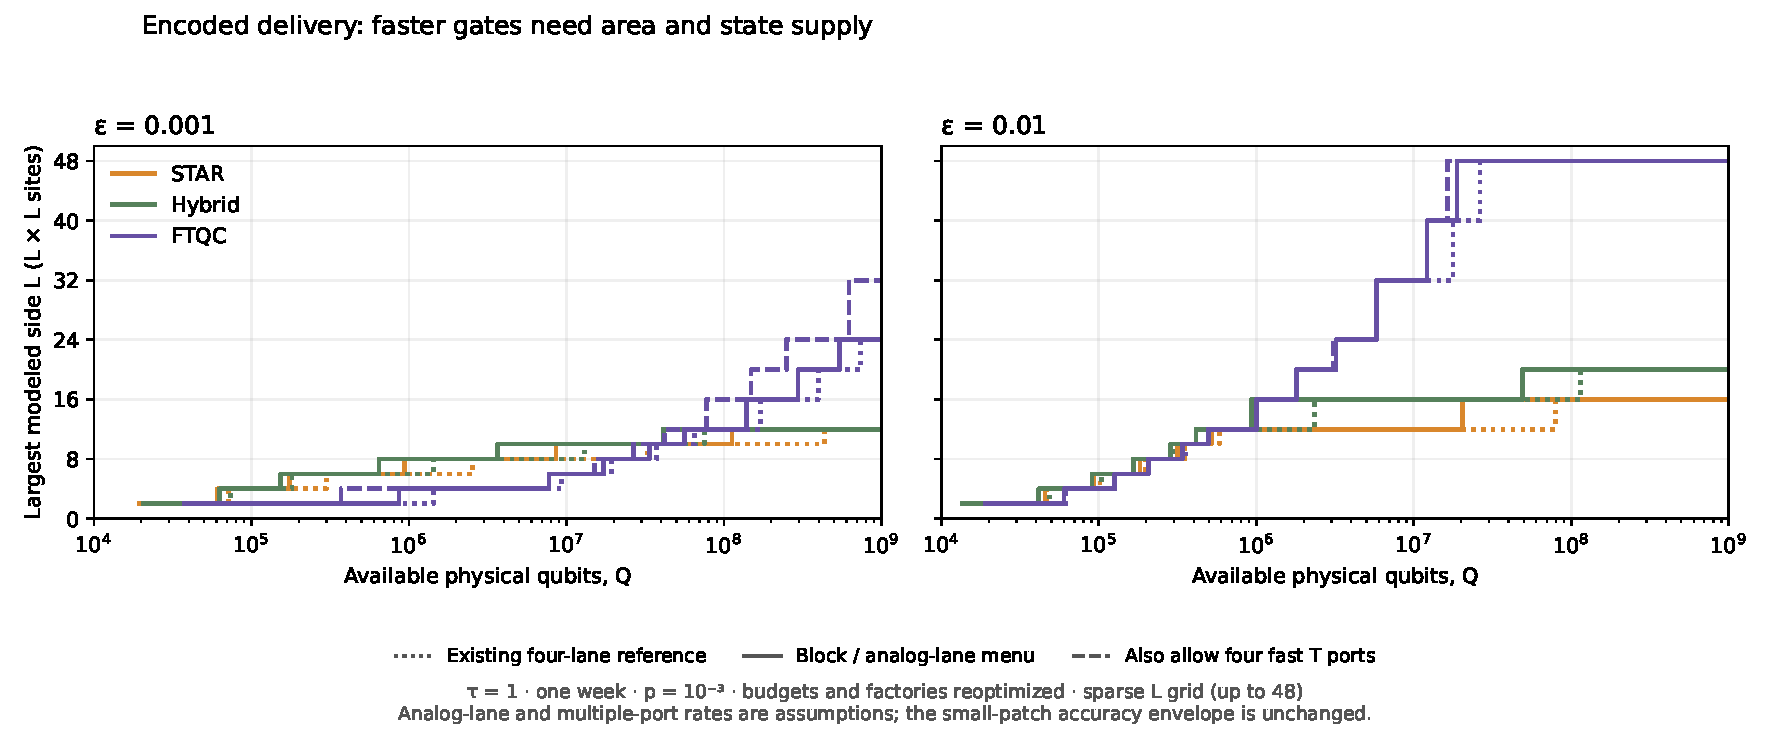
\includegraphics[width=\linewidth]{delivery_capacity.pdf}
\caption{Encoded capacity at $\tau=1$ after reoptimizing budgets and state
supply. The dotted reference retains four effective lanes. The solid menu
adds whole-block designs and analog-lane choices; the dashed menu also
allows four fast T ports. Menus are nested and share the expanded source
choices. Parallel rates are conditional assumptions. Staircases use only
the sampled sizes, with $L=48$ the sweep endpoint.}
\label{fig:delivery-capacity}
\end{figure}
\begin{figure}[t]
\centering
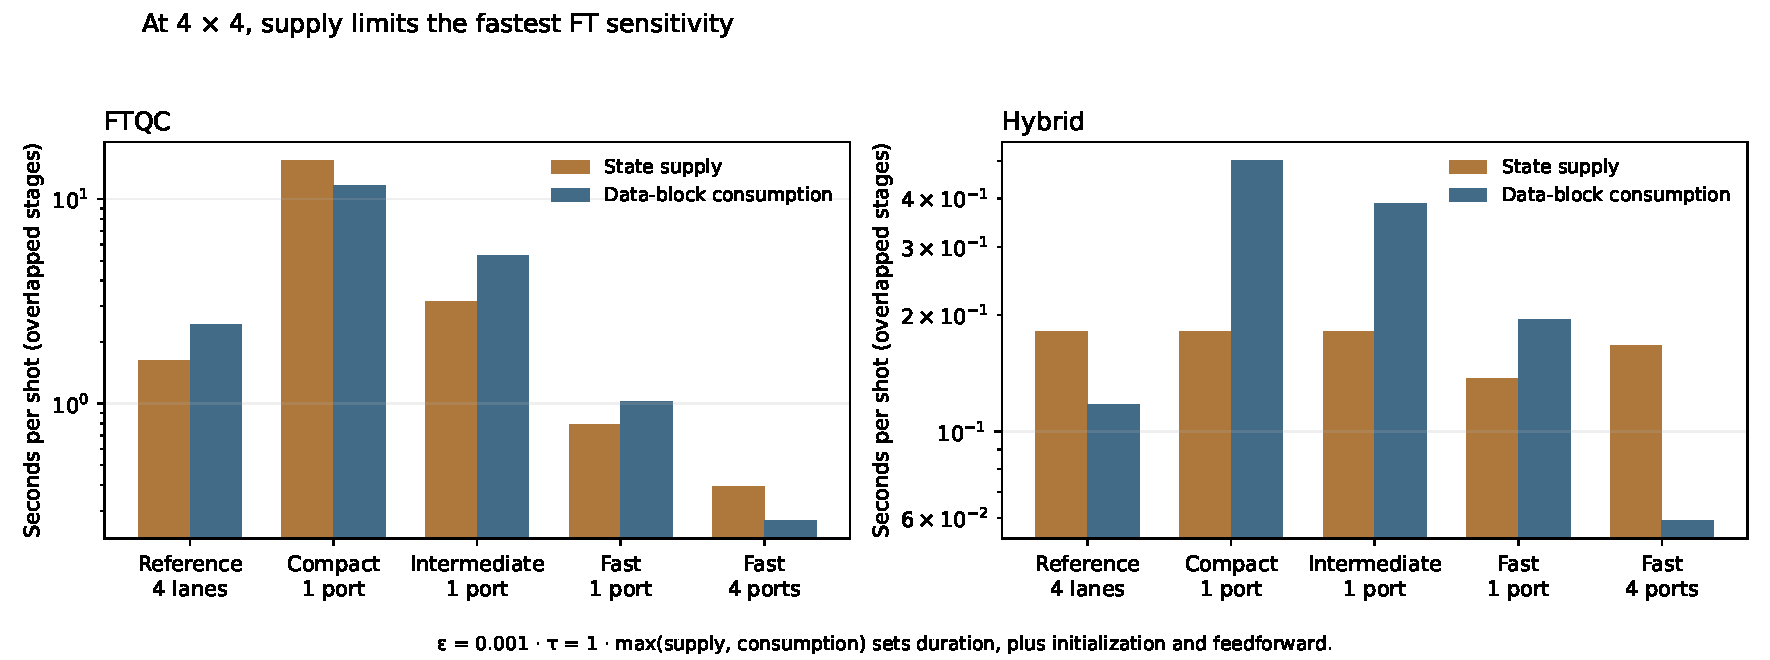
\includegraphics[width=\linewidth]{delivery_bottlenecks.pdf}
\caption{Supply and consumption durations at strict $4\times4$, $\tau=1$,
with each layout's budgets and source count reoptimized. These stages
overlap: their maximum enters shot time. The fastest FT sensitivity becomes
supply-limited, while the hybrid also pays for its analog rotations.}
\label{fig:delivery-bottlenecks}
\end{figure}
\subsection{Logical-fault commutation and its limitation}\label{app:c9}
A branch-independent fault channel $\mathcal F$ outside a complete PEC
cancellation block, or commuting through its noise channel $\mathcal E$,
satisfies $\mathcal E^{-1}\mathcal F\mathcal E=\mathcal F$. For a stochastic
fault of probability $q_L$, this gives bias at most $q_L$ for a $[0,1]$
observable. Pauli channels commute locally, making this a useful condition.
It does not follow merely from linearity or branch independence.

For a counterexample, take Bloch matrices
$E=\operatorname{diag}(s,s,1)$ and
$F=(1-q)I+qH$, where $H$ is Hadamard conjugation. On $|0\rangle$, measuring
$(I+X)/2$ after $E^{-1}FE$ gives bias $q/(2s)>q$ when $s<1/2$.
This is a stochastic non-Pauli fault inside the cancellation sandwich.
The logical STAR instrument of Section~\ref{M-sec:rus} instead verifies local
Z covariance under its stated Pauli fault model. A physical implementation
must justify that model across injection, growth, retries, and any selection
before the more favorable budget becomes its default.
\subsection{QSVT approximation and selection budget}\label{app:qsvt-budget}
For $x=\alpha\tau$, the Jacobi--Anger expansion has coefficients
$J_0(x)$ and $2(-i)^nJ_n(x)$. Truncation after degree $D$ has uniform
operator-error bound $2\sum_{n>D}|J_n(x)|$. We sum the finite Bessel tail
and bound the remainder using
$|J_n(x)|\leq(|x|/2)^n/n!$ and a geometric majorant. The even and odd
parts approximate cosine and sine, each divided by two; the branch LCU
divides by two again. The resulting block approximates $U/4$.
We reserve half of its error allowance for polynomial truncation and half
for classical phase realization. The latter is a required tolerance on
phase generation, not a numerical validation of every large-degree phase list.

After $j=0,1,2,3$ oblivious amplification steps, the accepted singular-value
polynomials are respectively
\begin{align}
 P_1(a)&=a, &P_3(a)&=3a-4a^3,\\
 P_5(a)&=5a-20a^3+16a^5, &
 P_7(a)&=7a-56a^3+112a^5-64a^7.
\end{align}
Their ideal amplitudes are $a_j=\sin[(2j+1)\arcsin(1/4)]$.
For a block error $\delta$, telescoping each matrix monomial gives
$\eta_j\leq C_j\delta$, where
$C_j=\sum_n n|c_n|(1/4+\delta)^{n-1}$ for $P_{2j+1}(a)=\sum_nc_na^n$.
The acceptance is at least $(a_j-\eta_j)^2$, and a conservative conditional
observable-error bound is $4\eta_j/(a_j-\eta_j)$.
Independent tests check both the amplification unitary and noncommuting
matrix perturbations. Rotation synthesis receives a further operator-error
allowance chosen with the same normalization bound. A stochastic circuit
fault of probability $q$ is charged at conditional bias $2q/P$ for acceptance
lower bound $P$, rather than using the deterministic-circuit bound $q$.
Shots include failed selection and a conservative fault-related acceptance
reserve. Resource estimates retain the reference synthesis fit and source
model, including cleanup when the selected budget requires it.


\subsection{The fixed-device question}
The same physical qubits can buy more simultaneous samples, stronger logical
protection, or faster delivery of non-Clifford operations. We want to determine
which use gives the largest accessible dynamics problem, and which combinations
can improve on the three reference approaches. Figure~\ref{M-fig:architectures}
shows the resource roles. The comparison includes physical probabilistic error
cancellation (PEC)~\cite{temme}, the original and small-angle STAR mechanisms~\cite{akahoshi,toshio}, and surface-code computation with explicit magic-state
supply~\cite{litinski,gidney2024cultivation}. Campbell's Hubbard construction
provides a concrete algorithmic baseline~\cite{campbell}; recent partial-FT
resource studies~\cite{chung} and a performed fermionic-dynamics experiment~\cite{alam2025} provide comparison points with distinct hardware assumptions.

We treat these as specified implementations and estimators. A poor physical
PEC curve is not an impossibility theorem for NISQ, and an encoded curve based
on reference patch timing is not a validated physical floorplan. The purpose
of the analytical laws is to expose the quantities whose measurement or
optimization can change the architecture ranking. CUDA-Q Logical supplies
explicit circuit and synthesis artifacts~\cite{cudaqlogical}; physical encoded
timing is kept separate when its implementation or verification is incomplete.


The similarity of the encoded data patches is physical: both approaches
protect their Clifford operations. The main distinction is how they supply
non-Clifford rotations, including the sequence of operations in time
(Figure~\ref{M-fig:rotation-protocols}). STAR teleports an angle-specific
resource state and mitigates residual rotation errors. Our FTQC reference
instead synthesizes the rotation from Clifford gates and high-fidelity T
states. In the original STAR preparation protocol, a surgery ancilla can
also serve as the preparation patch when distance and physical error rate
permit adequate acceptance~\cite[Sec.~II A 2]{toshio}. Preparation, any patch
growth, and retries still occupy space and time. Dedicated injection lanes
are therefore a scheduling choice in our cost model, not a defining STAR
requirement. Conversely, FTQC supply may be compact or shared in time;
neither approach has a universal ratio of data area to preparation area.

\subsection{Task, conventions, and precision}
The problem has $N=L^2$ Hubbard sites, $2N$ spin modes, and open boundaries.
The physical device has a separate area budget $Q$. In units where energies
are measured in $J$, we simulate
\begin{equation}\label{eq:H-v0}
 H/J=-\sum_{\langle ij\rangle,\sigma}
 (c^\dagger_{i\sigma}c_{j\sigma}+\mathrm{h.c.})
 +u\sum_i(n_{i\uparrow}-\tfrac12)(n_{i\downarrow}-\tfrac12),
 \qquad u=U/J=4.
\end{equation}
The symmetric onsite form differs from $U n_\uparrow n_\downarrow$ only
by a known phase in a fixed-number sector. We prepare the half-filled
N\'eel product state and measure the central doublon
$D=\langle n_{i\uparrow}n_{i\downarrow}\rangle$ at $\tau=Jt/\hbar$.
Doublon avoids the symmetry-pinned charge-density observable of this quench.

\begin{center}
\begin{tabular}{ll}
\toprule
Quantity & Reference value or convention\\
\midrule
Connectivity & Square array, nearest neighbors\\
Gate / measurement / reset & $10$ / $100$ / $100$ ns\\
Physical two-qubit / one-qubit error & $p=10^{-3}$ / $p/10$\\
Idle channel & Depolarizing error $p$ per $100$ ns\\
Encoded cycle / classical feedforward & $240$ / $200$ ns, reference assumptions\\
Runtime cutoff & $B=604800$ s, one week\\
Main precision & $1\%$ relative at provisional $D_*=0.1$: $\eps=0.001$\\
Statistical confidence & $1-\delta=0.95$\\
Rotation convention & $U_P(\theta)=e^{-i\theta P}$; CUDA-Q angle $\phi=2\theta$\\
\bottomrule
\end{tabular}
\end{center}
The native physical compilation assumes arbitrary-angle $R_{ZZ}$ and
one-qubit pulses at the stated gate duration. The noise channels and encoded
cycle are explicit model choices, not a characterization of a fabricated
device. In particular, the surface-code suppression fit has not been
calibrated to the same physical idle and syndrome schedule.

The target is $\eps=\eta|D|$ with $\eta=0.01$. Resource curves use the
declared signal $D_*$, rather than silently treating it as calculated dynamics.
Campbell's energy precision proportional to $N$ corresponds to fixed absolute
precision in energy density~\cite{campbell}. Our local $D$ is already
intensive: fixed absolute error in $D$ does not itself become stricter with
size. Relative precision is useful when the signal magnitude is the relevant
scale. Strict relative precision at zero signal needs a separate prescription;
a production estimator with unknown nonzero $D$ would require a pilot or
sequential confidence procedure. We retain $\eps=0.01$ absolute as a
separately labeled sensitivity.

We allocate fractions $(0.5,0.25,0.1,0.075,0.075)$ of $\eps$ to statistical,
algorithmic, logical, synthesis, and magic-state errors. For a spatial patch
$\Omega$ and product formula with $r$ steps,
\begin{equation}\label{eq:budget-v0}
 |\widehat D-D_{\mathrm{target}}|\leq\eps_{\mathrm{stat}}
 +|D_{\Omega,r}-D_\Omega|+|D_\Omega-D_{\mathrm{target}}|
 +\eps_{\mathrm{logical}}+\eps_{\mathrm{synth}}+\eps_{\mathrm{magic}}.
\end{equation}
The truncation scenario splits the existing $0.25\eps$ algorithmic reserve
equally between Trotter and spatial bias. It does not add a new allowance.
Mitigation assumes exact channel knowledge; a residual calibration bias would
need its own allocation within Eq.~\eqref{eq:budget-v0}. No unverified
postselection bias reduction is credited in a resource curve.

\subsection{Sampling, replication, and maximum lattice size}
For inverse channels $\mathcal E_j^{-1}=\sum_a c_{ja}\mathcal P_{ja}$,
define $\gamma_j=\sum_a|c_{ja}|$, $\Gamma=\prod_j\gamma_j$, and
$\chi=\log\Gamma^2$. Centering the doublon observable as $D-I/2$ puts
the PEC sample in $[-\Gamma/2,\Gamma/2]$. Hoeffding's bound then gives
\begin{equation}\label{eq:shots}
 n\geq\frac{\Gamma^2}{2\eps_{\mathrm{stat}}^2}\log\frac{2}{\delta},
 \qquad N_0=\left\lceil\frac{\log(2/\delta)}{2\eps_{\mathrm{stat}}^2}\right\rceil.
\end{equation}
At strict reference precision, $N_0=7377759$. This is a sufficient common
sampling convention, not a claim that every estimator needs this many shots.

Let $q_a$ and $t_a$ be the physical area and time of one complete sampler,
and let $a$ be whole-circuit acceptance. With $m=\lfloor Q/q_a\rfloor$ replicas,
\begin{equation}\label{eq:time}
 T_{\mathrm{answer}}\simeq\frac{N_0e^\chi t_a}{am},\qquad
 Q_{\min}(L)=q_a\max\!\left(1,
 \left\lceil\frac{N_0e^\chi t_a}{aB}\right\rceil\right).
\end{equation}
The code excludes a sampler whose single attempt exceeds $B$. Resource-state
rejection is charged in delivery time, not counted again as whole-circuit
rejection. Integer replicas are retained where they matter. Packing is an
area-budget reference; a global square placement, calibration overhead, and
control bandwidth are not yet modeled in the encoded curves.
For PEC, $Q_{\min}$ is the minimum replica area that meets this sufficient
sampling bound for the chosen implementation. It is not a lower bound on
the qubits needed by another estimator, or even a tight cost for this one.

The principal output is now
\begin{equation}\label{eq:lmax}
 L_{\max}^{\mathrm{tested}}(Q)=
 \max\{L\in\mathcal L_{\mathrm{tested}}:\min_s Q_{\min}(L,s)\leq Q\},
\end{equation}
where $s$ labels allowed distances, supply configurations, and lane counts.
This is a discrete upper envelope, not a smooth inverse fit. No feasible
tested lattice is left blank, and reaching the largest tested size is marked
as a survey boundary. We do not interpolate untested sizes or call that
boundary a physical saturation. The companion output
$\tau_{\max}(Q,L)$ follows by sweeping evolution time under the same contract;
it has not yet been accuracy-qualified.

\begin{figure}[t]
\centering
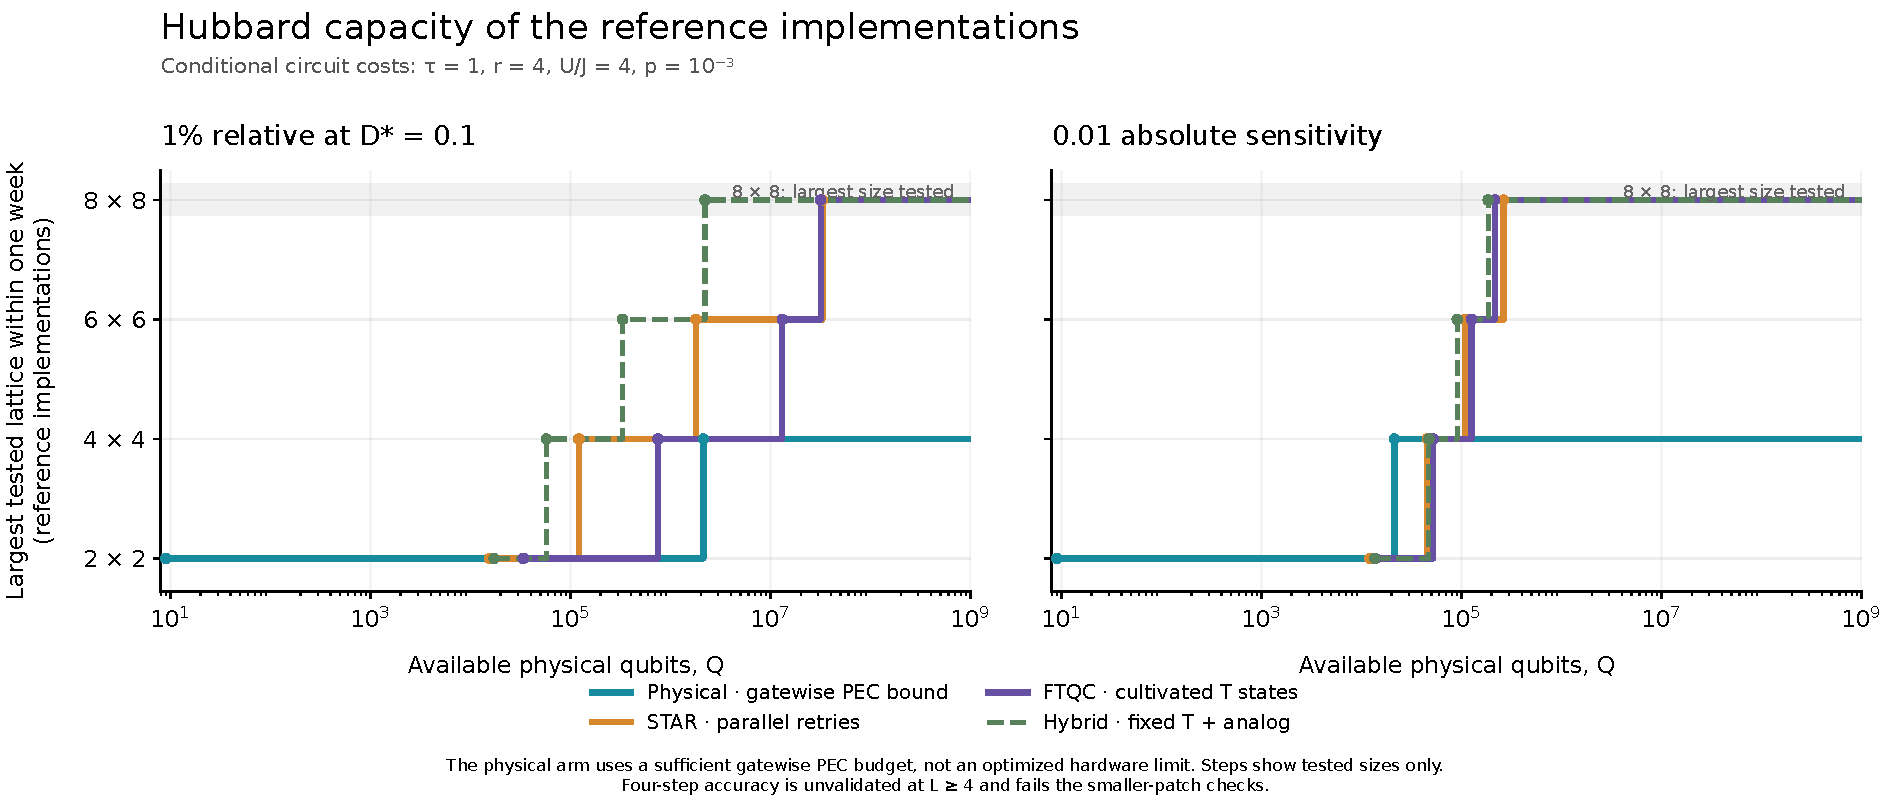
\includegraphics[width=\linewidth]{capacity_vs_qubits.pdf}
\caption{Largest tested Hubbard lattice within one week versus available
physical qubits. Left: the accepted relative-precision reference. Right: the
loose absolute-precision sensitivity. NISQ uses a sufficient gatewise-PEC
sampling bound on the compiled observable cone at nominal idle noise; it
does not represent optimized NISQ capacity. STAR chooses among one, two, four, and eight
reference injection lanes; FTQC and hybrid use the packed cultivation supply
scenario with zero additional handoff error. These are conditional $r=4$
costs, not accuracy-qualified dynamics capacities. That step count fails the
small square-patch checks, and $L\geq4$ accuracy is uncalibrated. The NISQ
compiler includes exact observable reductions that the encoded workloads have
not yet received. Only $L=2,4,6,8$ is tested; the upper band marks that limit.}
\label{fig:capacity}
\end{figure}

For a fixed circuit and estimator, Eq.~\eqref{eq:time} gives the exposure limit
\begin{equation}\label{eq:wall-v0}
 \chi\lesssim\log\frac{amB}{N_0t_a}.
\end{equation}
Increasing hardware or runtime therefore buys logarithmic exposure, even
though it can move a discrete lattice-size threshold appreciably. This is
the mitigation wall of the specified strategy, not a universal NISQ law.

\subsection{The common algorithm and its angle inventory}
\subsubsection{Termwise second order}
In a fixed-number sector, the single-$Z$ terms of the onsite interaction are
a known phase. With $E=2L(L-1)$ spatial bonds, the remaining Jordan--Wigner
Hamiltonian has
\begin{equation}
 K=4E+N=9N-8L,\qquad
 \lambda=\sum_\ell |h_\ell|=2E+\frac{|u|N}{4}=5N-4L.
\end{equation}
There are four hopping Pauli strings per spatial bond, each with coefficient
magnitude $1/2$, and one onsite $ZZ$ per site, with magnitude $|u|/4$.
Our convention is $U_P(\theta)=e^{-i\theta P}$; thus $R_z(\phi)$ has
$\phi=2\theta$, and a $T$ gate has $|\theta|=\pi/8$ up to a global phase.

For a symmetric product over the $K$ terms, choose onsite terms at both ends
of the ordering and merge adjacent identical rotations at the center and
between steps. Before further commuting or Clifford simplifications,
\begin{equation}\label{eq:termwise-v0}
 R_{\rm term}=r(2K-2)+1,\qquad \Theta_{\rm term}=\tau\lambda.
\end{equation}
The count follows from $r(2K-1)$ rotations after center merging and $r-1$
additional boundary merges. Every coefficient has total positive duration
$\tau$, proving the angle identity. Signed higher-order stages instead
multiply the angle sum by their total absolute stage weight. The histogram,
not merely $\Theta$, is retained for channel evaluation.

\subsubsection{Campbell plaquette second order with open boundaries}
Campbell partitions hopping into disjoint pink and gold tiles and applies
\begin{equation}\label{eq:plaq-v0}
 S_2(\Delta)=e^{-i\Delta H_I/2}e^{-i\Delta H_p/2}
 e^{-i\Delta H_g}e^{-i\Delta H_p/2}e^{-i\Delta H_I/2},
 \qquad \Delta=\tau/r.
\end{equation}
We adapt the periodic construction to open boundaries. The pink partition
has $P=L^2/4$ complete plaquettes. The shifted gold partition has
$G=(L/2-1)^2$ complete plaquettes and $B=2(L-2)$ isolated boundary bonds.
Each bond belongs to exactly one partition, since $4(P+G)+B=E$.

A single-spin four-site hopping cycle has eigenvalues $\{2,0,0,-2\}$.
Campbell's circuit implements its evolution with two variable-angle Pauli
rotations and eight fixed $T$ gates~\cite[Appendix E.1]{campbell}. An isolated
bond needs two commuting hopping Pauli rotations per spin. For $L\geq4$,
including both spin species and exact onsite boundary merging, this gives
\begin{align}
 R_{\rm plaq}&=N(r+1)+4r(2P+G+B),\\
 T_{\rm fixed}&=16r(2P+G),\\
 \Theta_{\rm dyn}&=\tau\left[\frac{|u|N}{4}+4(P+G)+2B\right].\label{eq:plaqangle-v0}
\end{align}
For $L=2$ the gold partition is empty: the two pink half steps merge, so
$2P$ becomes $P$ in the count formulas. The angle formula is unchanged.
At $L=4$, $\tau=1$, $r=4$, these formulas give
$(R_{\rm plaq},T_{\rm fixed},\Theta_{\rm dyn})=(288,576,44)$.

The compiled total angle includes $T_{\rm fixed}\pi/8$. Consequently, the
invariance of $\tau\lambda$ under refinement in Eq.~\eqref{eq:termwise-v0}
does not apply to all non-Clifford operations in Eq.~\eqref{eq:plaq-v0}.
The fixed basis changes are an algorithm-dependent STAR exposure even when
the variable rotations have no injection floor. Distilling those fixed
angles is an immediate hybrid candidate. Hamming-weight phasing, cancellations
between neighboring basis changes, and angle extraction remain further compiler
optimizations. Campbell neglects fermionic-swap Clifford costs in his
non-Clifford metric; our native nearest-neighbor compilation explicitly restores this motion.



\subsection{Encoded protection and the logical-fault budget}
Both encoded arms use the declared per-patch, per-cycle suppression reference
\begin{equation}\label{eq:logical-v0}
 p_L(d)=A(p/p_{\mathrm{th}})^{(d+1)/2},\qquad
 A=0.1,\quad p_{\mathrm{th}}=0.01.
\end{equation}
The alternative $(A,p_{\mathrm{th}})=(0.07,0.0039)$ is motivated by the
original STAR fit~\cite{akahoshi}. Its time convention and circuit noise
must be reconciled before it becomes a calibration of this device. We use
$240$ ns per syndrome cycle and roughly $2d^2$ physical qubits per tile as
reference accounting. Figure~\ref{fig:patch} distinguishes physical qubits,
logical patches, and operation/supply space.

For $V_L$ patch-cycles per attempt, $q_L\leq V_Lp_L(d)$ by a union bound.
A $[0,1]$ unmitigated observable has fault bias at most $q_L$. A uniform
branch-wise bound for centered PEC gives the sufficient worst-case
$\Gamma q_L$. Thus the reference chooses the smallest admissible odd $d$ with
\begin{equation}\label{eq:distance-v0}
 V_Lp_L(d)\leq\eps_L/\Gamma,\qquad
 d\gtrsim\frac{2\log(AV_L\Gamma/\eps_L)}{\log(p_{\mathrm{th}}/p)}-1.
\end{equation}
The implementation solves the discrete self-consistency problem because
duration and volume also depend on $d$. Faults are budgeted per attempt;
the full sampling campaign is not required to contain zero logical faults.
Commuting, branch-independent fault channels can justify removing $\Gamma$
locally. Section~\ref{M-sec:rus} checks this condition for a declared logical
injection instrument, and Appendix~\ref{app:c9} explains why independence
alone is insufficient.

\begin{figure}[t]
\centering
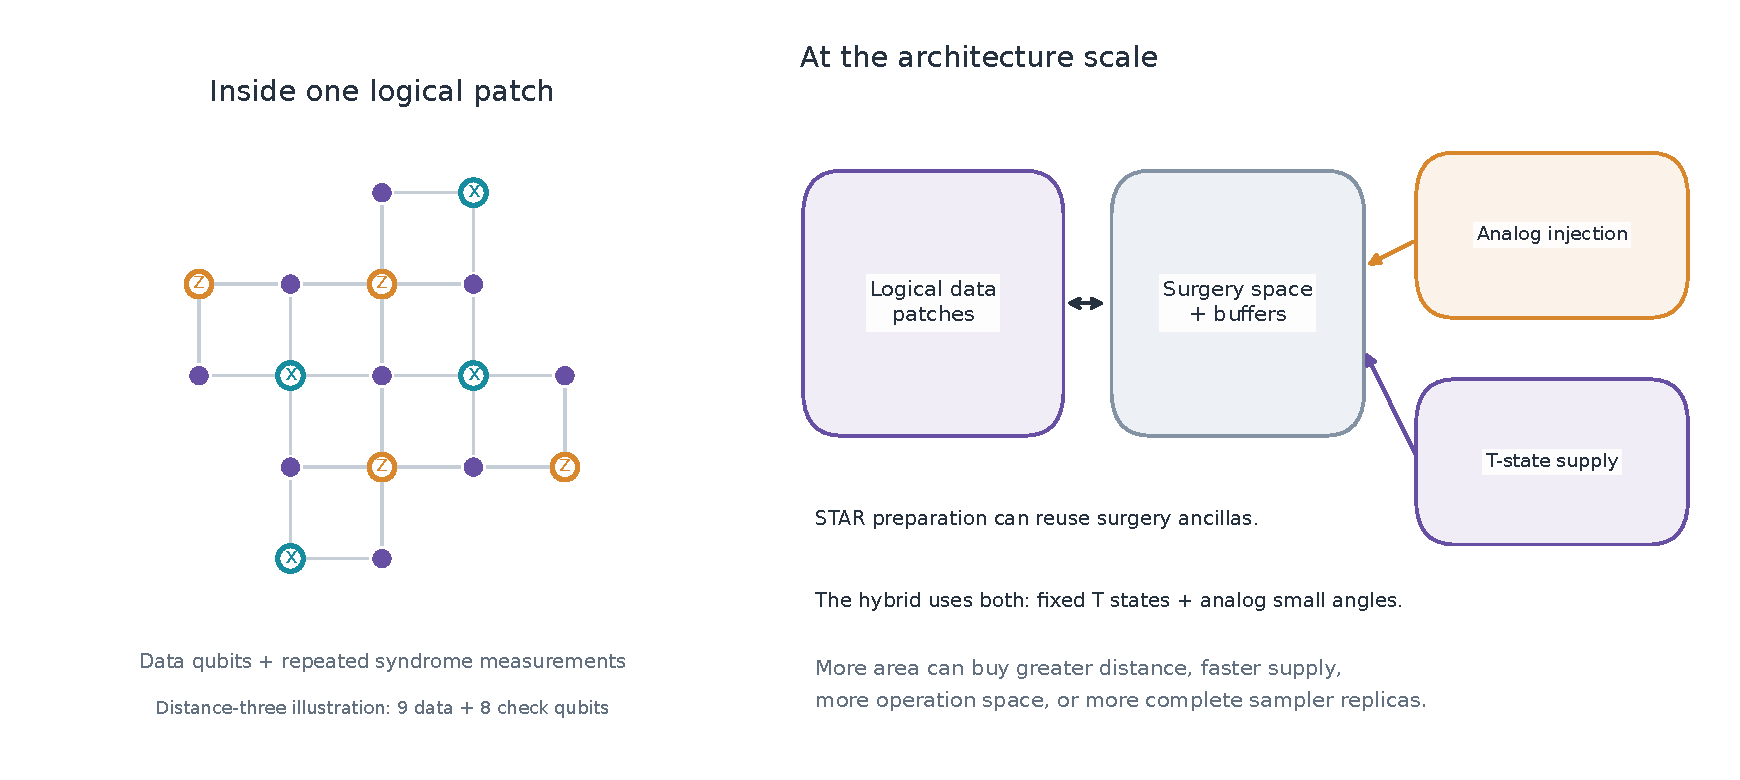
\includegraphics[width=\linewidth]{architecture_detail.pdf}
\caption{Physical and logical resource scales. Left: a distance-three
rotated-code illustration with nine data and eight check qubits; links are
nearest-neighbor data--check interactions. Right: logical data interacts
through operation space with analog injection or T-state supply. STAR and
FTQC use different supply paths; the hybrid uses both. The diagram shows
functional roles: STAR preparation can occupy surgery ancillas rather than
a separate supply region. This illustration is not a choice of distance or
a calibrated surgery schedule for the resource curves.}
\label{fig:patch}
\end{figure}

\subsection{What determines the scaling}
The exposure variables give a more transferable comparison than a single
crossover. With local full-lattice compilation, $R=O(Nr)$ and
$\Theta=O(N\tau)$. Physical PEC and original STAR therefore have reference
exponents $O(pNr)$, while the small-angle term has exponent $O(pN\tau)$.
An injection floor and the plaquette fixed-angle basis changes restore
$O(r)$ growth of the STAR exponent. Individual FT synthesis has
$N_T=O(Nr\log(Nr/\eps))$ and logarithmic distance growth below threshold,
but starts with a substantial protected footprint and supply overhead.
These are laws of the specified models, subject to the locality and accuracy
qualifications above.

The physical-error sweep in Figure~\ref{fig:p-capacity} improves the modeled
capacity of all three reference architectures as $p$ falls. The relative
ordering also depends on precision, injection floors, and source quality;
holding these quantities fixed or assigning improvement laws gives different
partial-FT windows. Figure~\ref{fig:hwp-capacity} identifies an algorithmic
change within FT that moves the strict-precision costs by approximately a
factor of six. The compact-encoding scenarios and ordering diagnostic show
why locality alone does not determine either the small-system gate count
or the Trotter coefficient.

The earlier compiled reference in Figure~\ref{fig:capacity} retains a
separate, conditional circuit comparison. At $Q=10^6$ and strict reference precision,
the largest tested conditional circuits are $2\times2$ for NISQ,
$4\times4$ for STAR and FTQC, and $6\times6$ for the hybrid. These numbers
use different implemented optimizations, conditional encoded supply, and
the same unqualified $r=4$ product formula. They are not final architecture
rankings. At loose precision the encoded thresholds cluster much more
closely, making delivery rate, distance, and integer replicas consequential.

Small-patch calibration explains why a common algorithmic correction does
not cancel from the resource comparison: increasing $r$ reduces a shared
Trotter error but enters each architecture's cost differently. Likewise,
physical truncation could reduce all three arms if its bias is controlled.
Direct $4\times4$ checks now settle the Trotter component for the selected
headline workloads. The remaining scientific dependencies are transfer of
accuracy to larger lattices, a controlled spatial truncation estimate,
empirical NISQ mitigation bias, and physical injection/growth and
handoff schedules with residual-channel validation. The same-Hamiltonian
qubitization comparison in Section~\ref{sec:qsvt-comparison} does not
reverse the tested ordering; its routed implementation and tighter
state-dependent locality bounds remain unvalidated.



\section{Earlier calibrations}\label{sup:calibration}
\subsection{Capacity sensitivity to the finite-patch envelope}
To isolate this physics input, we keep the reference delivery assumptions
and the expanded common source menu fixed and reoptimize the resource
budgets under two coefficient policies. The first is the earlier
$3\times3$ envelope. The second retains that envelope and adds all
measured $4\times3$ and $4\times4$ coefficients through the requested
time, including finite-step corrections, with the same $10\%$ margin.
The $L=2$ point keeps its own calibration in both cases.
Figure~\ref{fig:patch-capacity} reports the resulting capacity sensitivity.
It does not replace a finite-patch assumption with a bulk error bound:
the new curves still transfer coefficients to $L>4$, and their optimized
step counts have not all been checked directly. No $4\times4$ coefficient
is inferred at $\tau=8$.
The additional patches move several discrete thresholds while retaining
the strong precision dependence in this reference model. For example,
at $\tau=2$, $Q=10^6$, and strict precision, effective NISQ falls from
$L=4$ to $L=2$, whereas reference STAR and hybrid remain at $L=4$.
This is a sensitivity to the assumed mitigation and finite-patch models;
it is not a general NISQ limit.

\begin{figure}[t]
\centering
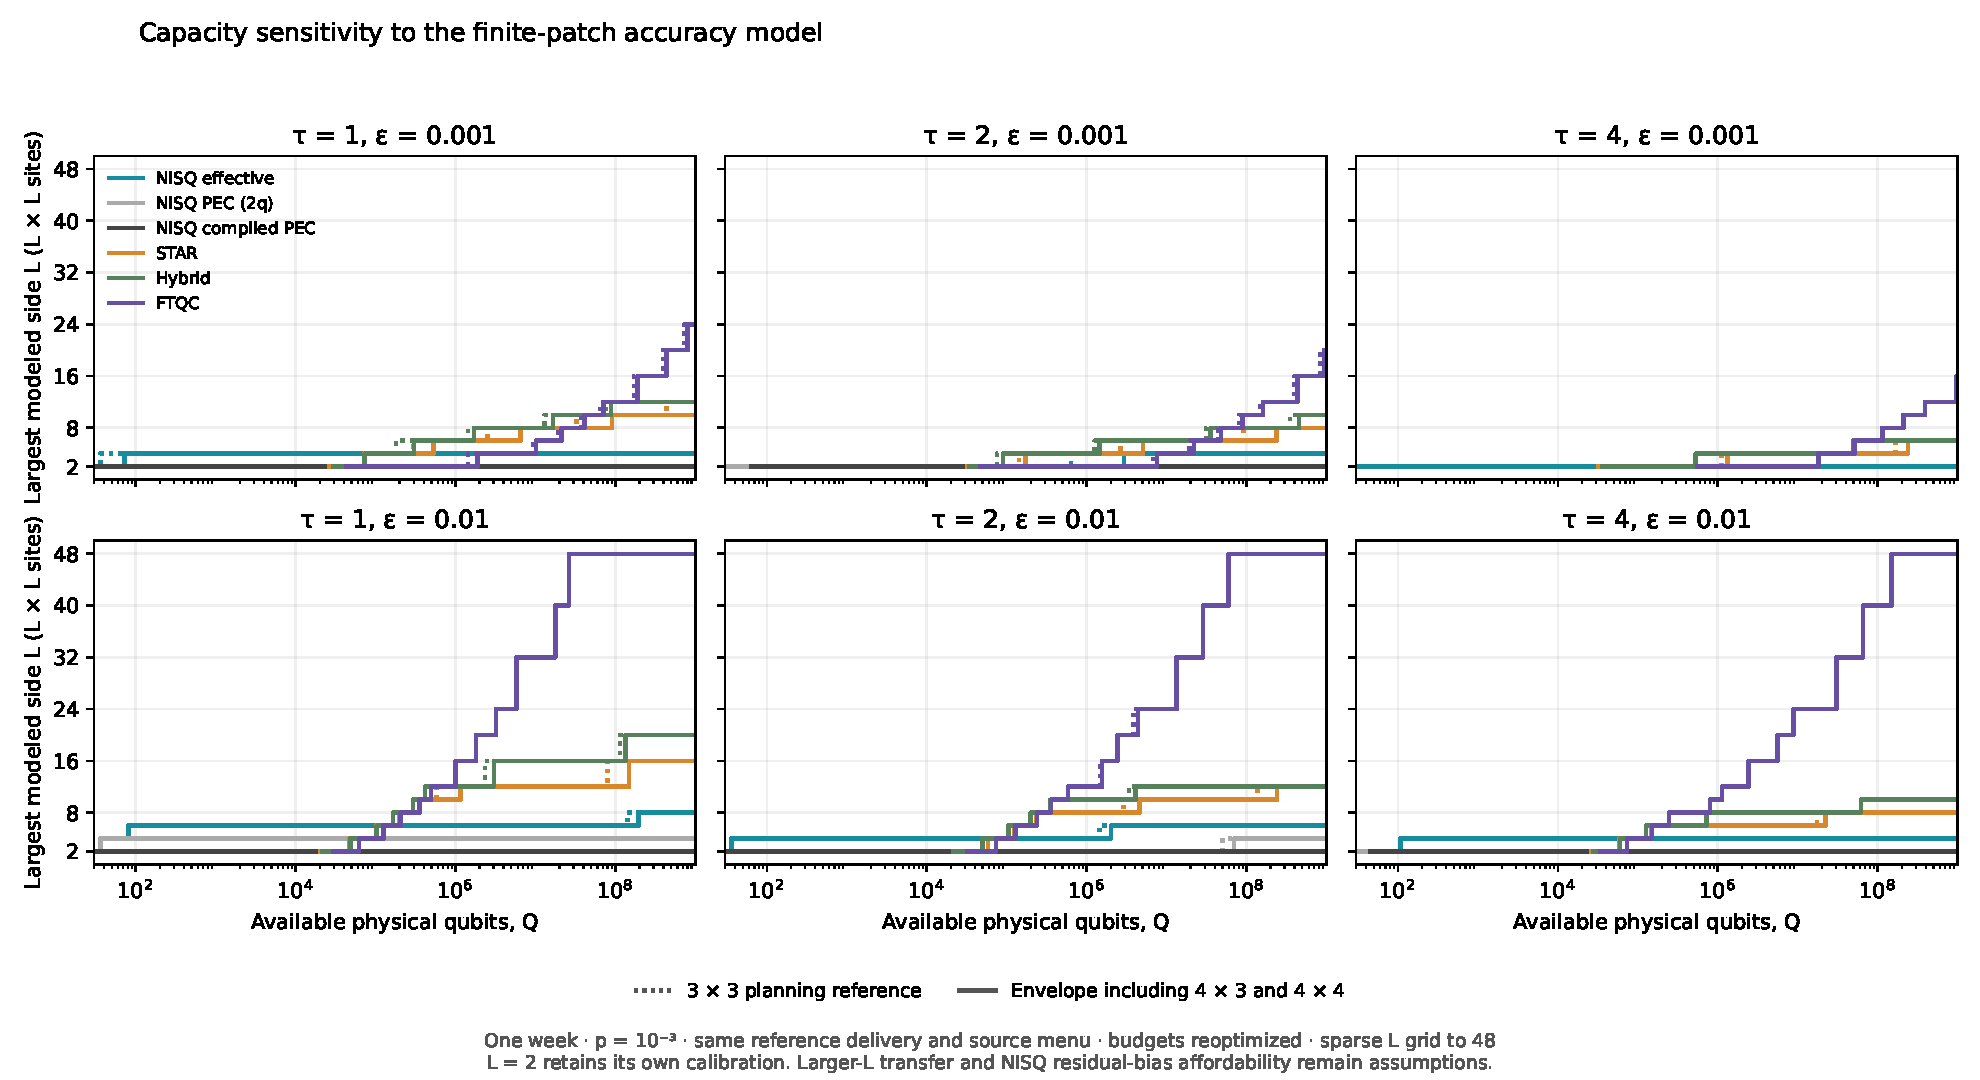
\includegraphics[width=\linewidth]{patch_capacity.pdf}
\caption{Largest modeled lattice side versus available qubits, changing
only the finite-patch accuracy model. Dotted curves use the original
$3\times3$ envelope; solid curves also include the $4\times3$ and
$4\times4$ measurements. Delivery and source menus are identical, with
error allocations reoptimized. Both policies retain direct $L=2$
calibration. NISQ effective mitigation remains an assumed envelope;
two-qubit-only PEC and the full compiled-noise PEC proxy are shown
alongside it. All curves use a one-week cutoff, $p=10^{-3}$, and
the same sparse size grid through $L=48$. A missing curve means that no
sampled lattice fits that panel's qubit and time budgets.}
\label{fig:patch-capacity}
\end{figure}

\subsection{Accuracy, truncation, and noisy observables}\label{sec:calibration}
The calibration constructs $H$ directly in fixed $(N_\uparrow,N_\downarrow)$
sectors. Sparse matrix exponentiation evaluates $e^{-i\tau H/J}$ without using
the compiled gate decomposition. A separate evolution applies
\begin{equation}
 U_r(\tau)=\left[
 e^{-i\Delta H_U/2}
 e^{-i\Delta H_{\mathrm{pink}}/2}
 e^{-i\Delta H_{\mathrm{gold}}}
 e^{-i\Delta H_{\mathrm{pink}}/2}
 e^{-i\Delta H_U/2}\right]^r,
 \qquad \Delta=\tau/r,
\end{equation}
where energies are in units of $J$. The largest patch is $3\times3$, with
sector dimension $\binom94\binom95=15876$. An independent eight-qubit dense
Hamiltonian verifies the exact-sector observable; the original compiled
plaquette circuit independently verifies the product formula on $2\times2$.
The saved evidence contains $112$ Trotter comparisons and $164$ exact-curve
points over four patches.

\begin{center}
\begin{tabular}{lrrrr}
\toprule
Patch, $\tau=1$ & Exact $D$ & Error $r=4$ & Error $r=16$ & Error $r=64$\\
\midrule
$2\times2$ & $0.1179790$ & $0.0136397$ & $0.00087075$ & $0.00005447$\\
$3\times3$ & $0.1050849$ & $0.0143939$ & $0.00085350$ & $0.00005317$\\
\bottomrule
\end{tabular}
\end{center}
For these square patches, $r=64$ is the first tested power of two passing the
strict split budget; $r=16$ passes the loose split budget. These are not
minimal-step claims. The asymptotic local error is consistent with $r^{-2}$,
while coarse steps can be nonmonotonic. We also record a budget based on $1\%$
of each actual patch signal, rather than silently replacing the provisional
$D_*$ in every resource curve.

The compiled $L=2$ circuits at $r=4,16,64$ contain respectively $164,740,3044$
native entanglers. The selected PEC estimator needs only one nine-qubit square
copy at $r=16$, but approximately $4.73\times10^6$ qubits at $r=64$ to meet
the week cutoff. Thus a common Trotter refinement can affect architecture
costs very differently: it increases a physical noise exposure in an
exponential, even when its algorithmic error reduction is shared. The
corresponding $L=4$ compilations demonstrate cost sensitivity only; their
Trotter error has not been calibrated.

To start testing physical truncation, compare a five-site cross with its
enclosing $3\times3$ square, keeping the same N\'eel pattern and central
observable. Their exact differences are $4.75\times10^{-4}$ at $\tau=0.1$
and $7.93\times10^{-2}$ at $\tau=1$. Both exceed the strict truncation
allowance. However,
\begin{equation}
 |D_{\mathrm{cross}}-D_{\mathrm{target}}|
 \leq |D_{\mathrm{cross}}-D_{3\times3}|
       +|D_{3\times3}-D_{\mathrm{target}}|,
\end{equation}
and the second term is unknown. These finite-reference differences neither
certify a bulk light cone nor bound the error of the larger patch. Larger
patches, controlled local bounds, or both are still needed.

\begin{figure}[t]
\centering
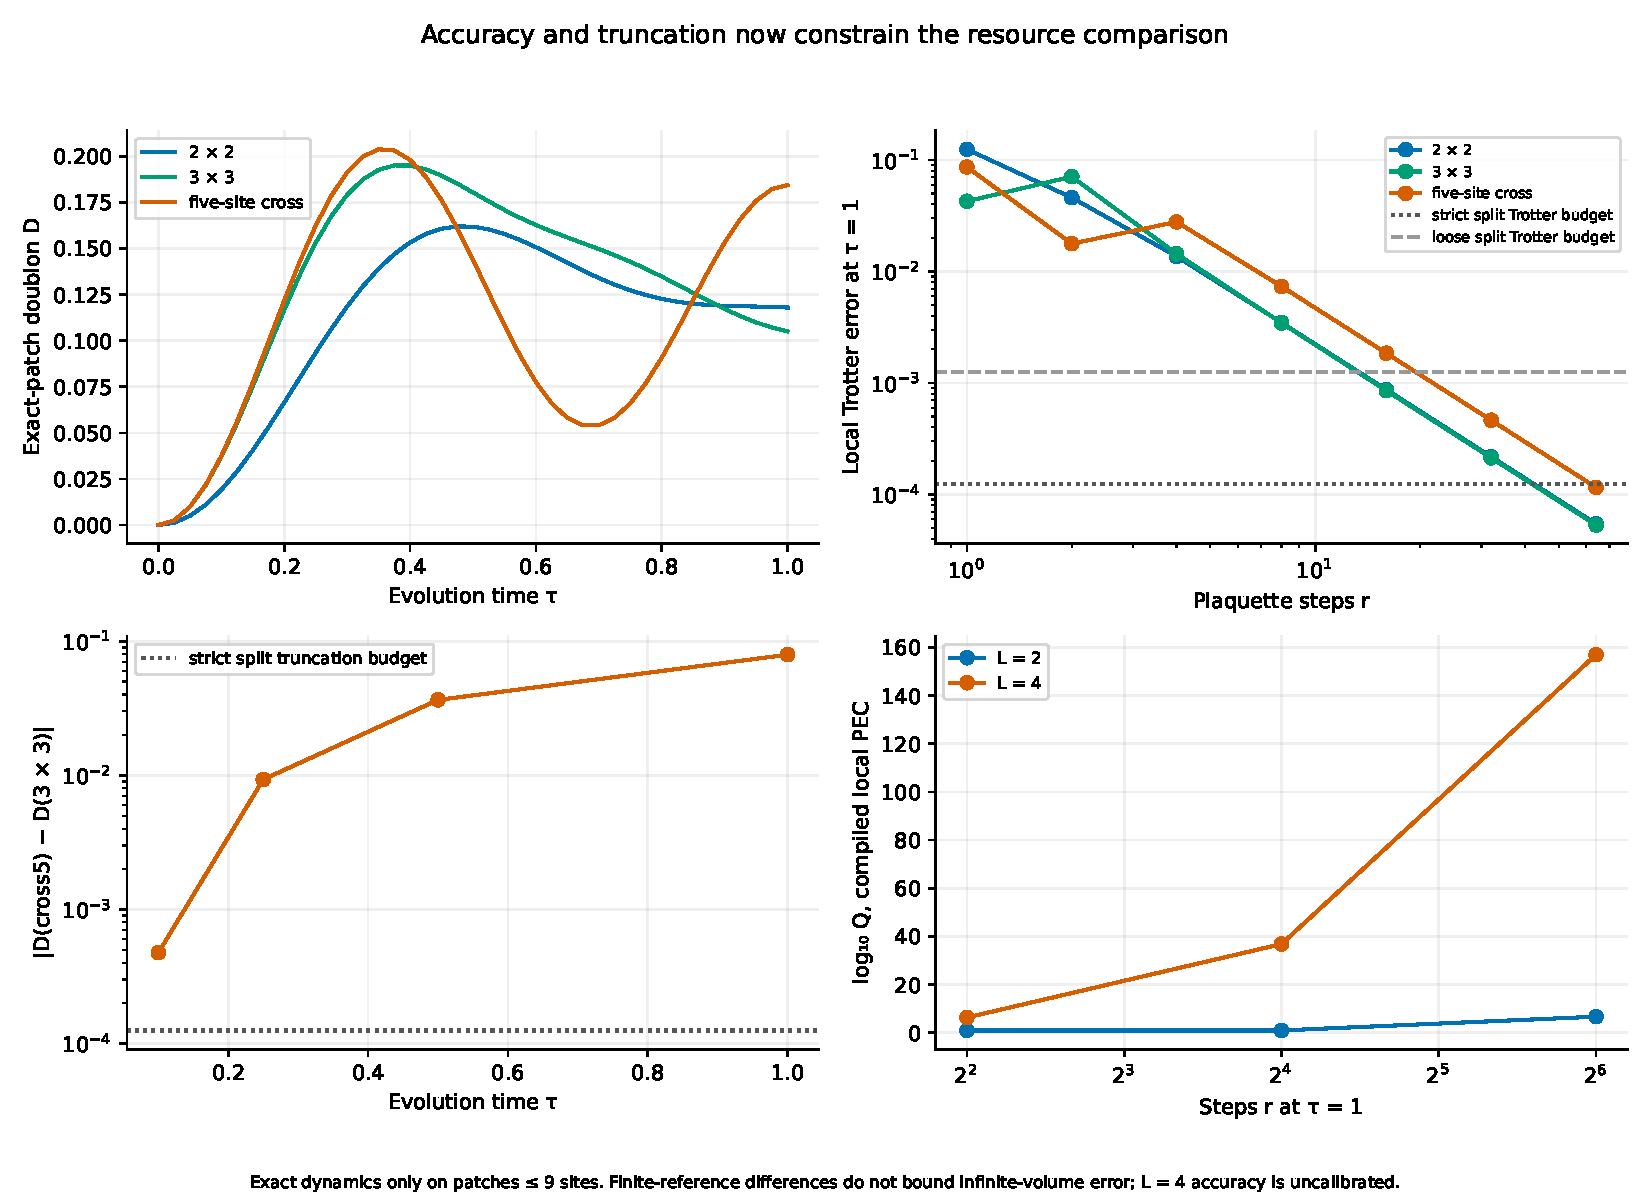
\includegraphics[width=\linewidth]{results/refinement_v3/accuracy_calibration.pdf}
\caption{Exact patch dynamics, local product-formula errors, a nested spatial
comparison, and the cost sensitivity to $r$. Each exact curve belongs to its
own finite patch. The spatial difference is not an infinite-volume error
certificate. The $L=4$ cost sweep does not assume the small-patch error law
holds at $L=4$.}
\end{figure}

\subsubsection{Postselection: measuring bias as well as acceptance}
We propagate the full eight-qubit density matrix through the saved $L=2$
native circuits. After each $k$-qubit primitive, the channel is
\begin{equation}
 \mathcal D_{k,p}(\rho)=(1-p)\rho+
 \frac{p}{4^k-1}\sum_{P\ne I}P\rho P.
\end{equation}
Primitive idle channels, initial preparation flips, and final readout flips
are also included. A direct Pauli-mixture implementation independently checks
the optimized channel calculation. For selection event $A$, the measured
quantity is $D_A=\mathbb E[D\mathbf1_A]/\Pr(A)$; a large or small acceptance
alone says nothing sufficient about its bias.

At $r=4$, the unselected noise bias relative to the ideal Trotter circuit is
$0.020371$. Selecting the two spin parities reduces it to $0.005808$ with
acceptance $0.81958$. Selecting exact $N_\uparrow=N_\downarrow=2$ reduces it
to $0.004212$ with acceptance $0.80943$. Its bias relative to exact dynamics,
including the independently measured Trotter error, is $0.01785$. At $r=64$,
the number-selected noise bias rises to $0.1070$. Postselection helps here,
but by itself does not meet the strict precision target.

The parity acceptance agrees with the independently propagated Pauli-character
formula. Trace errors are below $1.4\times10^{-12}$ and the calculated density
matrices remain positive. These results apply to the stated eight-qubit
circuits and noise channels. They do not prove failure of selection at $L=4$
or of combinations with other mitigation methods. The larger trapped-ion
experiment~\cite{alam2025} remains a separate circuit, geometry, and noise
comparison.

\begin{figure}[t]
\centering
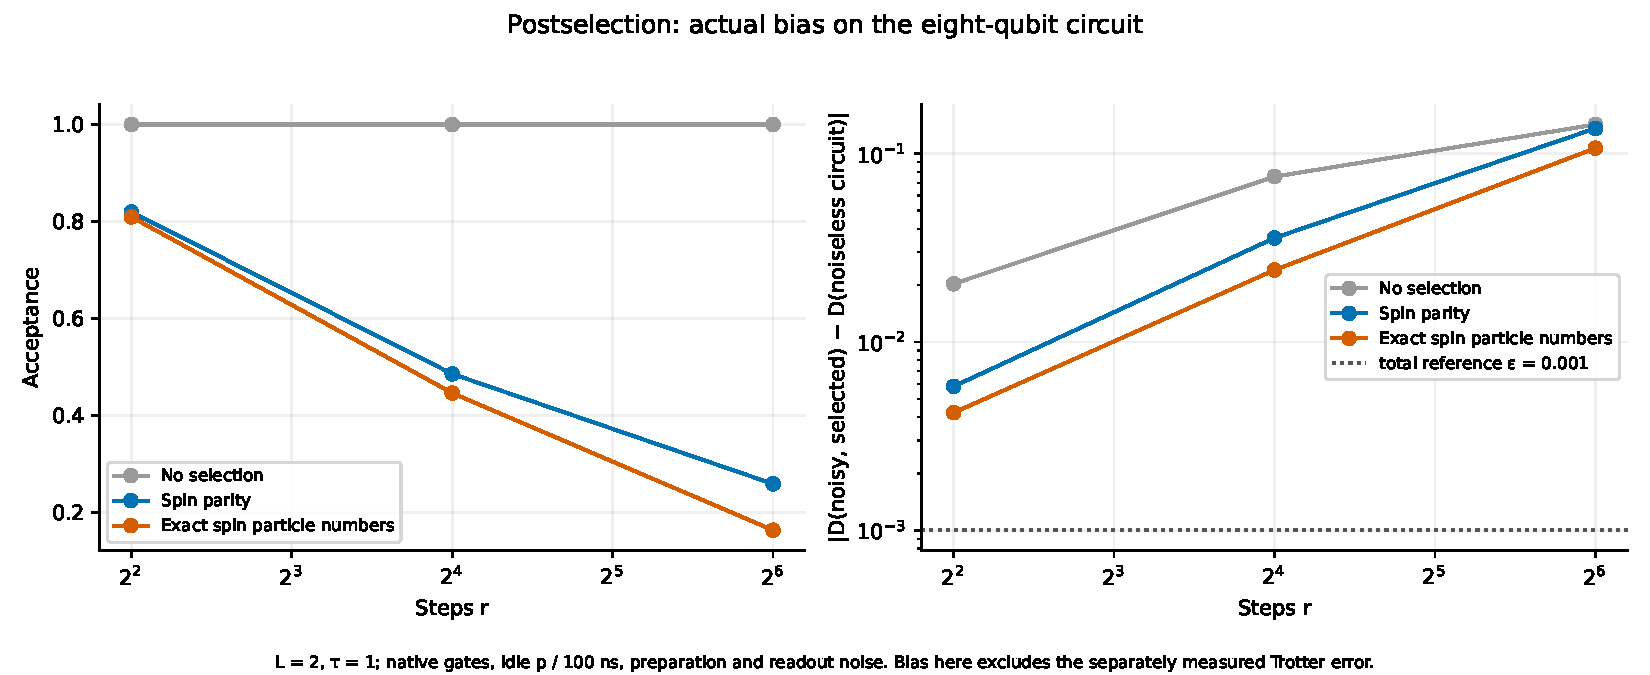
\includegraphics[width=\linewidth]{results/refinement_v3/postselection_bias.pdf}
\caption{Exact acceptance and actual observable bias under the declared
eight-qubit noise model. The right panel isolates noise bias from Trotter
bias. No extrapolation from these curves to $L\geq4$ is used.}
\end{figure}


\subsection{A conservative centered truncation bound}\label{app:local-certificate}
In the interaction picture of the onsite terms, each even hopping operator
remains supported on its two sites and keeps norm $2J$. Disjoint even
fermionic operators commute, so the usual commutator recursion applies
without interpreting Jordan--Wigner strings as physical propagation.
Duhamel's formula expresses the difference between full and truncated
Heisenberg observables as an integral over omitted boundary bonds.
Iterating the commutator recursion inside the retained patch produces a
chain of overlapping bonds terminating at that boundary. A chain of length
$n$ contributes at most $\|D-I/2\|(4|\tau|)^n/n!$.
There are at most $4\cdot7^{n-1}$ such chains before imposing the endpoint
condition, and no boundary-reaching chain has $n<R+1$. Summing gives
Eq.~\eqref{eq:local-certificate}. Time dependence in the interaction picture
does not change the uniform norm or ordered-simplex bounds.
For $x=28|\tau|$ and $R+2>x$, the numerical implementation uses
\begin{equation}
 \sum_{n\geq R+1}\frac{x^n}{n!}
 \leq \frac{x^{R+1}}{(R+1)!}\frac{1}{1-x/(R+2)}.
\end{equation}
The operator-norm bound also bounds the expectation difference for consistent
initial reduced states. Values use double precision with a small positive
roundoff margin; no interval-arithmetic certification is claimed.


\section{Compilation, checks, and reproducibility}
The installed CPU CUDA-Q Logical environment compiles the common analog
program, native physical circuits, and synthesized Clifford+T words.
The physical routes carry mode permutations, explicit nearest-neighbor gates,
ASAP schedules, counts, and hashes. The STAR retry program contains real
logical preparation, measurement, and conditional angle doubling with an
exhaustion flag. These P0 artifacts do not imply a physical STAR QEC schedule.

The installed minimal surface recipe lacks some needed gate gadgets.
An explicit encoded macro adapter reaches physical IR, but the Hubbard
backend timing is rejected. A reduced circuit with four fixed-angle
rotations repeated four times, totaling $16$ T states, triggers a nested
schedule interval error. The $4$-, $8$-, and $32$-T variants pass a loose
bound, and separate two-resource template-call controls return their
expected times. The root cause remains unresolved. None of these backend
timings enters the resource curves; passing the loose controls is not a
validation of physical encoded timing.

Tests independently check fermionic signs, product-formula identities,
synthesis accuracy, exact-sector dynamics, primitive Pauli noise, STAR
instrument algebra, and resource budgets. The capacity inversion additionally
checks threshold inclusion, nonmonotone cost envelopes, and the untested
region. These checks validate the specified calculations rather than the
hardware assumptions.

The repository entry point is \texttt{README.md}. Source code is in
\texttt{python/}, tests in \texttt{tests/}, assumptions in \texttt{configs/},
and this manuscript in \texttt{tex/main.tex} with a dedicated
\texttt{tex/references.bib}. Current overview figures are in \texttt{figures/};
versioned scientific evidence stays in \texttt{results/}. Earlier complete
notes are in \texttt{tex/archive/}. The original v3 manifest is preserved:
historical source hashes are checked against their archived snapshots, while
the relocated code replays the same saved numerical evidence. The presentation
manifest records the new figures and their source datasets without relabeling
older results as a new calculation.

\bibliographystyle{unsrt}
\bibliography{references}
\end{document}
